%%%%%%%%%%%%%%%%%%%%%%%%%%%%%%%%%%%%%%%%%
% Beamer Presentation
% LaTeX Template
% Version 1.0 (10/11/12)
%
% This template has been downloaded from:
% http://www.LaTeXTemplates.com
%
% License:
% CC BY-NC-SA 3.0 (http://creativecommons.org/licenses/by-nc-sa/3.0/)
%
%%%%%%%%%%%%%%%%%%%%%%%%%%%%%%%%%%%%%%%%%

%----------------------------------------------------------------------------------------
%	PACKAGES AND THEMES
%----------------------------------------------------------------------------------------

\documentclass[aspectratio=169, 9pt]{beamer}

\mode<presentation> {

% The Beamer class comes with a number of default slide themes
% which change the colors and layouts of slides. Below this is a list
% of all the themes, uncomment each in turn to see what they look like.

%\usetheme{default}
%\usetheme{AnnArbor}
%\usetheme{Antibes}
%\usetheme{Bergen}
%\usetheme{Berkeley}
%\usetheme{Berlin}
%\usetheme{Boadilla}
%\usetheme{CambridgeUS}
%\usetheme{Copenhagen}
%\usetheme{Darmstadt}
%\usetheme{Dresden}
%\usetheme{Frankfurt}
%\usetheme{Goettingen}
%\usetheme{Hannover}
%\usetheme{Ilmenau}
%\usetheme{JuanLesPins}
%\usetheme{Luebeck}
%\usetheme{Madrid}
\usetheme{Malmoe}
%\usetheme{Marburg}
%\usetheme{Montpellier}
%\usetheme{PaloAlto}
%\usetheme{Pittsburgh}
%\usetheme{Rochester}
%\usetheme{Singapore}
%\usetheme{Szeged}
%\usetheme{Warsaw}

% As well as themes, the Beamer class has a number of color themes
% for any slide theme. Uncomment each of these in turn to see how it
% changes the colors of your current slide theme.

%\usecolortheme{albatross}
%\usecolortheme{beaver}
%\usecolortheme{beetle}
%\usecolortheme{crane}
%\usecolortheme{dolphin}
%\usecolortheme{dove}
%\usecolortheme{fly}
%\usecolortheme{lily}
%\usecolortheme{orchid}
%\usecolortheme{rose}
%\usecolortheme{seagull}
%\usecolortheme{seahorse}
%\usecolortheme{whale}
%\usecolortheme{wolverine}

%\setbeamertemplate{footline} % To remove the footer line in all slides uncomment this line
%\setbeamertemplate{footline}[page number] % To replace the footer line in all slides with a simple slide count uncomment this line

%\setbeamertemplate{navigation symbols}{} % To remove the navigation symbols from the bottom of all slides uncomment this line
}

\usepackage{xcolor}

\definecolor{han_purple}{rgb}{0, 0.28, 0.80}
\definecolor{beige}{rgb}{0.96, 0.92, 0.89}
\definecolor{lightgray}{rgb}{0.8, 0.8, 0.8}
\definecolor{blue}{HTML}{3066be}
\definecolor{green}{HTML}{43894e}
\definecolor{definition}{HTML}{0ABD1C}
\definecolor{theorem}{HTML}{0072A3}
\definecolor{proposition}{HTML}{FF4B3E}
\definecolor{orange}{HTML}{F5B400}
\definecolor{purple}{HTML}{30CC71}
\definecolor{red}{HTML}{eb9486}
\definecolor{lightgreen}{HTML}{72d5a3}
\definecolor{darkgreen}{HTML}{216e47}


\newcommand{\X}{\boldsymbol{X}}
\newcommand{\V}{\boldsymbol{V}}
\newcommand{\W}{\boldsymbol{W}}
\newcommand{\Y}{\boldsymbol{Y}}
\newcommand{\Q}{\boldsymbol{Q}}
\newcommand{\Z}{\boldsymbol{Z}}
\newcommand{\M}{\boldsymbol{M}}
\newcommand{\A}{\boldsymbol{A}}
\renewcommand{\H}{\boldsymbol{H}}
\newcommand{\B}{\boldsymbol{B}}
\newcommand{\D}{\boldsymbol{D}}
\newcommand{\R}{\boldsymbol{R}}
\renewcommand{\P}{\boldsymbol{P}}
\newcommand{\I}{\boldsymbol{I}}
\renewcommand{\L}{\boldsymbol{\Lambda}}
\renewcommand{\S}{\boldsymbol{\Sigma}}

\DeclareMathOperator*{\argmax}{arg\,max}
\DeclareMathOperator*{\argmin}{arg\,min}

\definecolor{physics}{HTML}{8EA604}
\definecolor{intrinsic}{HTML}{ec9f05}
\definecolor{semantic}{HTML}{818AA3}

%\definecolor{azure}{HTML}{728797}
\definecolor{coral}{HTML}{566876}
\definecolor{pin}{HTML}{005556}
\definecolor{pousse}{HTML}{00b57b}
\definecolor{ardoise}{HTML}{5b6770}

\usepackage{comment}
\usepackage{subcaption}
\usepackage{bibentry}
\usepackage{amsmath}
\usepackage{tabularray}[=v2021]
\usepackage{hyperref}

%\DeclareMathOperator*{\max}{arg\,min}
%\DeclareMathOperator*{\min}{arg\,max}

\usepackage{multirow}
\usepackage{enumitem}
\usepackage{subcaption}
\usepackage{makecell}
\usefonttheme[onlymath]{serif}
\usepackage{booktabs}
\usepackage{mathabx}
\usepackage{amssymb}

\usepackage{animate}

\newcommand{\x}{\boldsymbol{x}}
\newcommand{\z}{\boldsymbol{z}}
\newcommand{\param}{\boldsymbol{\theta}}
\newcommand{\phiparam}{\boldsymbol{\phi}}
\newcommand{\qphi}{q_{\phiparam}}
\newcommand{\zi}{\textcolor{red}{\z_I}}
\newcommand{\ze}{\textcolor{blue}{\z_E}}
\newcommand{\xk}[1]{\boldsymbol{x}^{(#1)}}
\newcommand{\yk}[1]{y^{(#1)}}
\newcommand{\vv}{\boldsymbol{v}}
\newcommand{\ppdf}{p_{\boldsymbol{\theta}}}
\newcommand{\fphi}{f_{\boldsymbol{\phi}}}

\renewcommand{\L}{\textcolor{blue}{L}}
\newcommand{\PW}{\textcolor{red}{PW}}


\newtheorem{thm}{Théorème}

\setbeamertemplate{page number in head/foot}[appendixframenumber] % stop page numebering after conclusion

\setbeamercolor{section in head/foot}{bg=coral!50!black, fg=white}
\setbeamercolor{frametitle}{fg=ardoise}
\setbeamercolor{structure}{fg=pin}
\setbeamercolor{title}{fg=ardoise}

\hypersetup{
    colorlinks,
    linkcolor={ardoise},
    citecolor={blue!80!black},
    urlcolor={ardoise}
}

%\hypersetup{colorlinks,urlbordercolor={1 1 1},linkcolor=,urlcolor=poussin}

%\setbeamercolor{footline}{bg=pin, fg=pin}

\newenvironment{madridblock}[1]
{
  \begin{block}{#1}
}
{
  \end{block}
}

\titlegraphic{
    
\includegraphics[height=0.8cm]{figures/logo_mia.png} \hspace{0cm}
    
\includegraphics[height=0.6cm]{figures/APT_Logo_RVB_Positif.png} \hspace{0cm}
    
\includegraphics[height=0.8cm]{figures/Logotype UPSaclay_RVB.png}
}

%\setbeamercolor{block title}{bg=coral!40,fg=black}
%\setbeamercolor{block body}{bg=coral!5,fg=black}

%\hypersetup{
%    colorlinks,
%    citecolor=han_purple,
%    linkcolor=han_purple
%}

%\newcommand{\vv}[1]{\textcolor{han_purple}{#1}}
%
%\DeclareFontFamily{U}{matha}{\hyphenchar\font45}
%\DeclareFontShape{U}{matha}{m}{n}{
%      <5> <6> <7> <8> <9> <10> gen * matha
%      <10.95> matha10 <12> <14.4> <17.28> <20.74> <24.88> matha12
%      }{}
%\DeclareSymbolFont{matha}{U}{matha}{m}{n}

\setbeamercovered{transparent}

\setbeamertemplate{headline}{}

\makeatletter
\def\normalcolor{\let\current@color\default@color\set@color\transparent{1}}
\makeatother
%----------------------------------------------------------------------------------------
%	TITLE PAGE
%----------------------------------------------------------------------------------------
\title{Remote sensing in practice: from the visible to the infrared for forest monitoring}
\subtitle{UC ATHENS}

\author[Romain Thoreau]{
	Romain Thoreau \\ AgroParisTech - MIA Paris Saclay
	\\ \url{romain.thoreau@agroparistech.fr}
}

\institute[AgroParisTech]

\date{November 2026}


%\setbeamertemplate{footline}{}
\setbeamertemplate{navigation symbols}{}

\setbeamertemplate{footline}
{
  \leavevmode%
  \hbox{%
  \begin{beamercolorbox}[wd=.333333\paperwidth,ht=2.25ex,dp=1ex,center]{author in head/foot}%
    \usebeamerfont{author in head/foot}\insertshortauthor
  \end{beamercolorbox}%
  \begin{beamercolorbox}[wd=.333333\paperwidth,ht=2.25ex,dp=1ex,center]{title in head/foot}%
    \usebeamerfont{title in head/foot}\insertshortinstitute
  \end{beamercolorbox}%
  \begin{beamercolorbox}[wd=.333333\paperwidth,ht=2.25ex,dp=1ex,right]{date in head/foot}%
    \usebeamerfont{date in head/foot}\insertshortdate{}\hspace*{2em}
    \insertframenumber{} / \inserttotalframenumber\hspace*{2ex} 
  \end{beamercolorbox}}%
  \vskip0pt%
}


\setbeamercolor{textcitation}{fg=black,bg=beige}
\setbeamerfont{block body textcitation}{size=\tiny}

\begin{document}
%--------------------------------------------------------------------------
\begin{frame}
\titlepage % Print the title page as the first slide
\end{frame}
%%%-------------------------------------------------------------------------
\begin{frame}{Outline}
\tableofcontents
\end{frame}
%---------------------------------------------------------------------------
\section{Why did you choose this course?}
%---------------------------------------------------------------------------
\section{Presentation of the course}
%---------------------------------------------------------------------------
\subsection{Schedule}
%---------------------------------------------------------------------------
\begin{frame}{Organization of the course}

\textbf{Schedule} \quad \L = \textcolor{blue}{Lecture} \quad \PW = \textcolor{red}{Practical Work} \quad AM = 8:30 - 11:45 \quad PM = 13:30 - 16:45 \\ \vspace{0.3cm}
\begin{tabular}{lcl}
	Monday & AM & Introduction to remote sensing (\L)\\
		   &  & The basics of radiative transfer modeling (\PW) \\
		   & PM & Inversion of leaf traits from satellites images (\PW) \\
		   & & \\
	Tuesday & AM & Co-registration of satellite images (\PW) \\
		    & PM & Interpolation of satellite time series (\PW) \\
		    & & \\
	Wednesday & AM & Anomaly detection for forest monitoring (\L) \\
			 & & Start of the project \\
			 & PM & Group work outside class \\
			 & & \\
	Thursday & AM & Project in class \\
			& PM & Group work outside class\\
			& & \\
	Friday & AM & Project in class \\
	& & Uploading of your detection model on the website \\
	& PM & Team presentation of the projects (\textcolor{green}{evaluation})
\end{tabular}

\end{frame}
%---------------------------------------------------------------------------
\subsection{Learning objectives}
%---------------------------------------------------------------------------
\begin{frame}{Learning objectives}
This course will cover theoretical concepts of \textbf{remote sensing} using
\textbf{optical imagery} ranging from the visible to the short-wavelength infrared (0.4 µm–2.5 µm) with a focus on the practical \textbf{processing
of satellite images} to detect \textbf{tree dieback} caused by bark beetle infestations. \vspace{0.4cm}

By the end of the week, you will be able to:
\begin{itemize}[label=$\bullet$]
	\item \textbf{Select} optical remote sensing data suitable \textbf{for a given application},
	\item \textbf{Process} optical satellite images using \textbf{specialized Python libraries},
	\item \textbf{Select and apply an anomaly detection method} for forest monitoring.
\end{itemize}

\begin{figure}
	\center
	\begin{subfigure}{0.2\textwidth}
		\center
		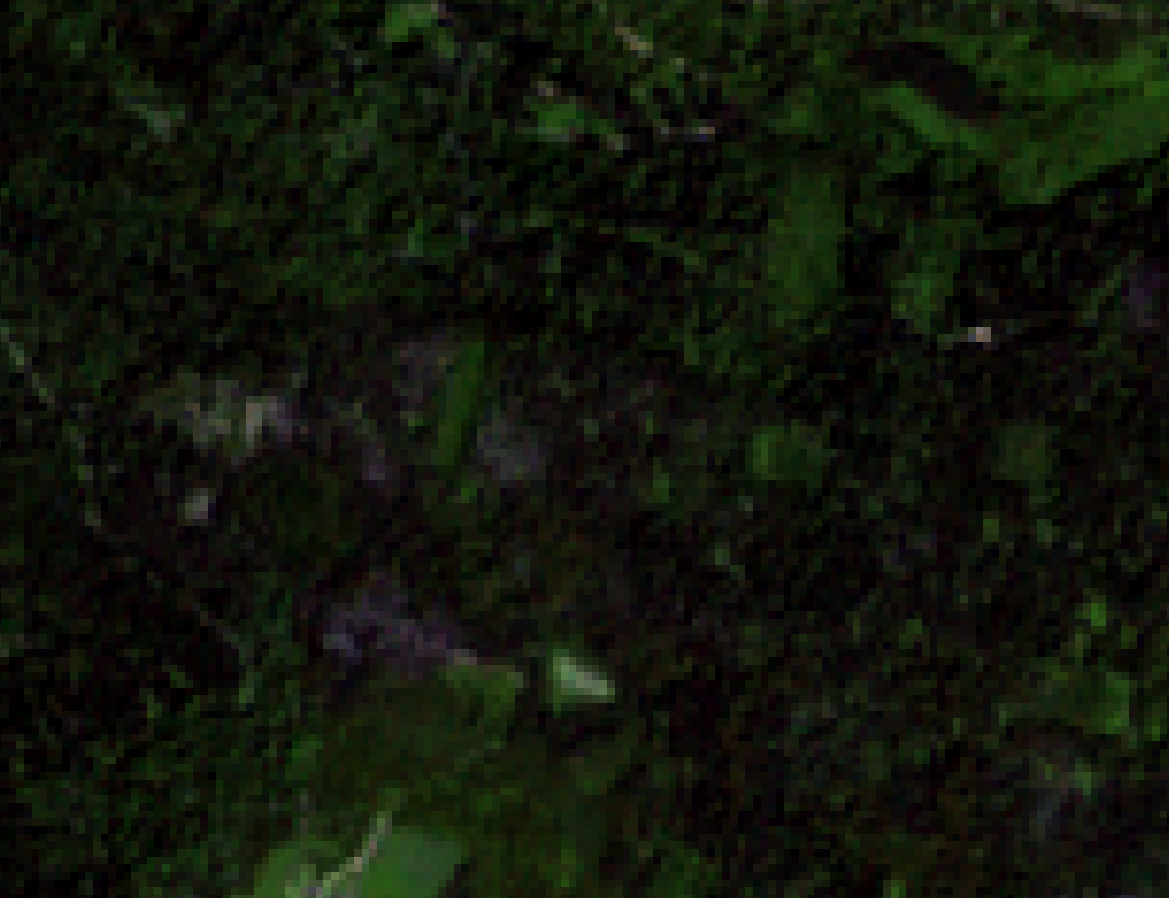
\includegraphics[width=\textwidth]{figures/ajol_2018.png}
		\caption{2018}
	\end{subfigure}
	\begin{subfigure}{0.2\textwidth}
		\center
		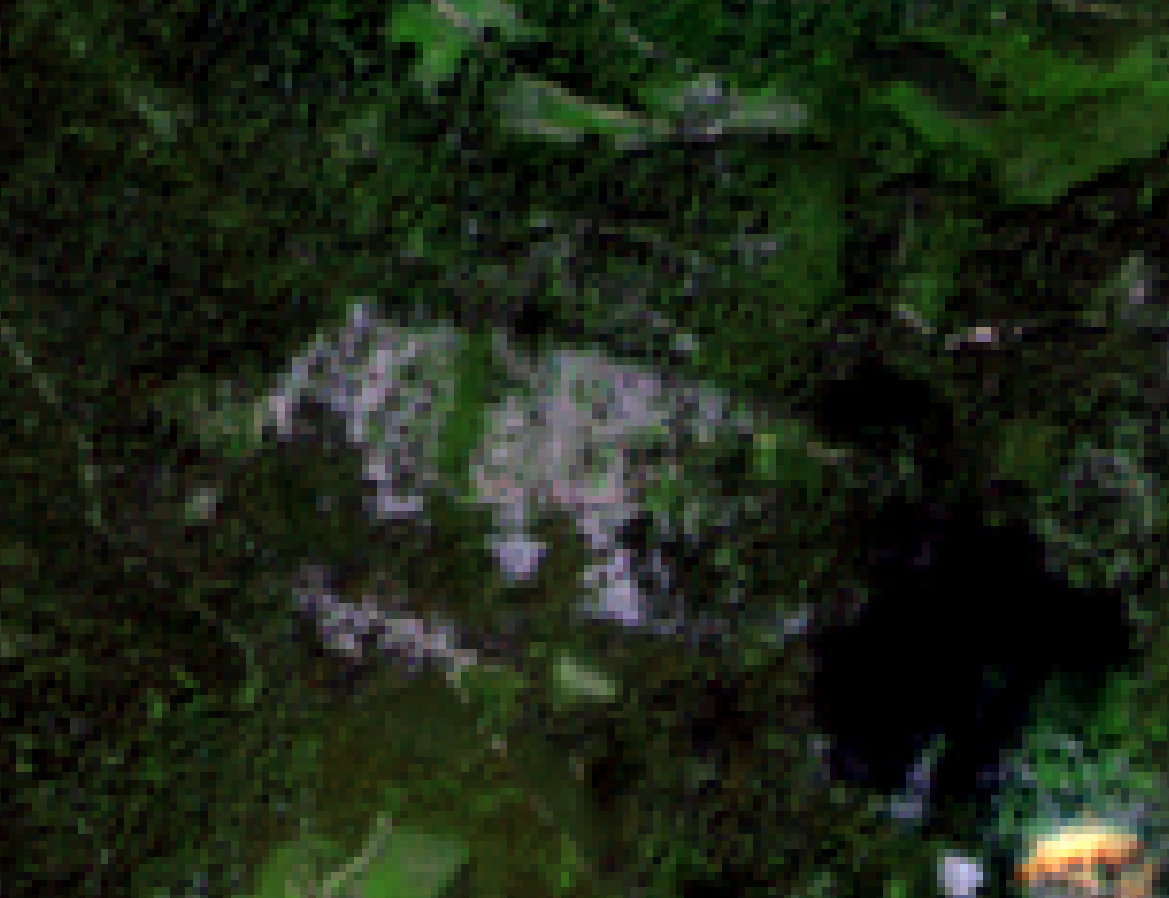
\includegraphics[width=\textwidth]{figures/ajol_2019.png}
		\caption{2019}
	\end{subfigure}
	\begin{subfigure}{0.2\textwidth}
		\center
		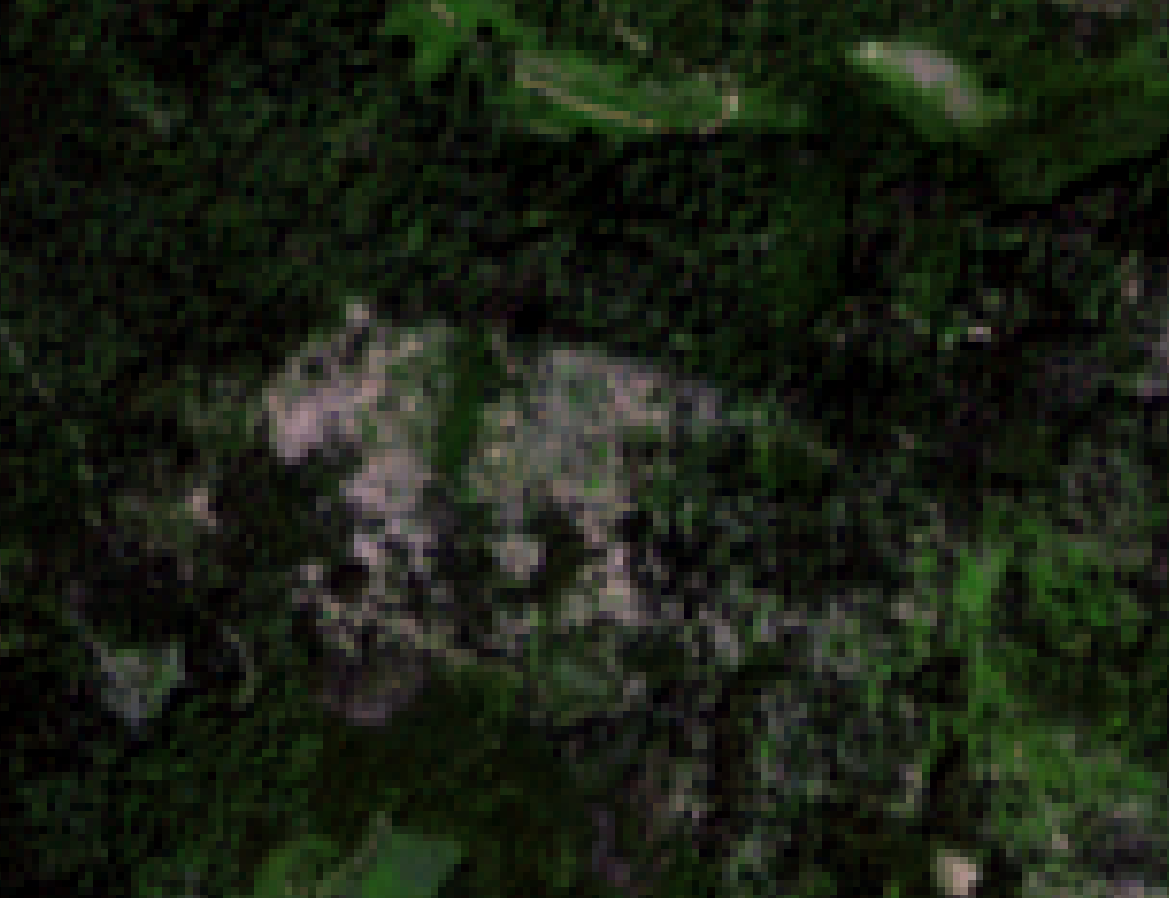
\includegraphics[width=\textwidth]{figures/ajol_2020.png}
		\caption{2020}
	\end{subfigure}
	\caption{RGB composition of Sentinel-2 images (ESA, Copernicus) - Val d'Ajol, France}
\end{figure}
\end{frame}

%---------------------------------------------------------------------------
\subsection{My academic background}
%---------------------------------------------------------------------------
\begin{frame}{My academic background}

%\begin{tabular}{lll}
%	2020-23 & \makecell[l]{ONERA \\ Magellium \\ Institut de Mathématiques de Toulouse \\ ISAE-SUPAERO} & PhD in computer science on the automatic mapping of impervious surfaces in cities from airborne hyperspectral images
%\end{tabular}

\begin{tabular}{lll}
    2016-20 & \textbf{Engineering Degree and Research Master's} \\
    & \textit{Arts et Métiers ParisTech \& Pierre and Marie Curie University} \\
    & \\
    2020-23 & \textbf{PhD in computer science} on the automatic mapping of impervious surfaces \\
    & in cities from airborne hyperspectral images \\
    & \textit{ONERA, Magellium, Institut de Mathématiques de Toulouse, ISAE-SUPAERO} \\
    & \\
    2024-25 & \textbf{Postdoctoral research in computer science} on the analysis of multi-source \\
    & satellite images for wildfire prediction \\
    & \textit{CNES, Laboratoire Sciences pour l'Environnement - Université de Corse - CNRS} \\
    & \\
    2025- & \textbf{Assistant Professor (Maître de Conférences) in computer science} \\
    & Analysis of multi-source satellite data for the monitoring of industrial pollution \\
    & and agricultural crops \\
    & \textit{AgroParisTech}
\end{tabular}

\end{frame}
%---------------------------------------------------------------------------
\subsection{Bibliography and references}
%---------------------------------------------------------------------------
\begin{frame}{Bibliography and references used for this lecture}

\begin{itemize}[label=$\bullet$]
	\item Lecture (in French) "Le rayonnement, sa mesure et son rôle - Modélisation du Transfert Radiatif", J.P. Gastellu-Etchegorry, \url{https://www.cesbio.cnrs.fr/dart/documentation/},
	\item Lecture (in French) "Télédétection et géophysique spatiale", Stéphane Jacquemoud, \url{http://step.ipgp.fr/images/2/20/Cours.pdf},
	\item Lecture on Atmospheric Transmission, Simon A. Carn, \url{https://pages.mtu.edu/~scarn/teaching/GE4250/transmission_lecture.pdf},
	\item CESBIO's blog: \url{https://www.cesbio.cnrs.fr/multitemp/}
\end{itemize}

\end{frame}
%---------------------------------------------------------------------------
\section{General Introduction to Remote Sensing}
%---------------------------------------------------------------------------
\subsection{Historical background}
%---------------------------------------------------------------------------
\begin{frame}{Outline}
\tableofcontents[currentsection, currentsubsection]
\end{frame}
%---------------------------------------------------------------------------
\begin{frame}{Early developments during the two world wars\footnote{\url{https://www.esa.int/SPECIALS/Eduspace_FR}, \url{https://fr.wikipedia.org/wiki/Programme_spatial_fran\%C3\%A7ais}}}

\begin{itemize}[label=$\blacktriangleright$]
    \item \textbf{First World War}
    The beginnings of airborne remote sensing: ordinary cameras are mounted on reconnaissance aircraft.
    \item \textbf{Second World War}
    \begin{itemize}[label=\textemdash]
        \item Mapping of coastal areas in preparation for the D-Day landings (water depth, enemy positions, camouflage nets),
        \item The German V2 surface-to-surface ballistic missile contains all the components of future space launchers.
    \end{itemize}
\end{itemize}

\begin{columns}

\column{0.45\textwidth}

\begin{figure}
    \center
    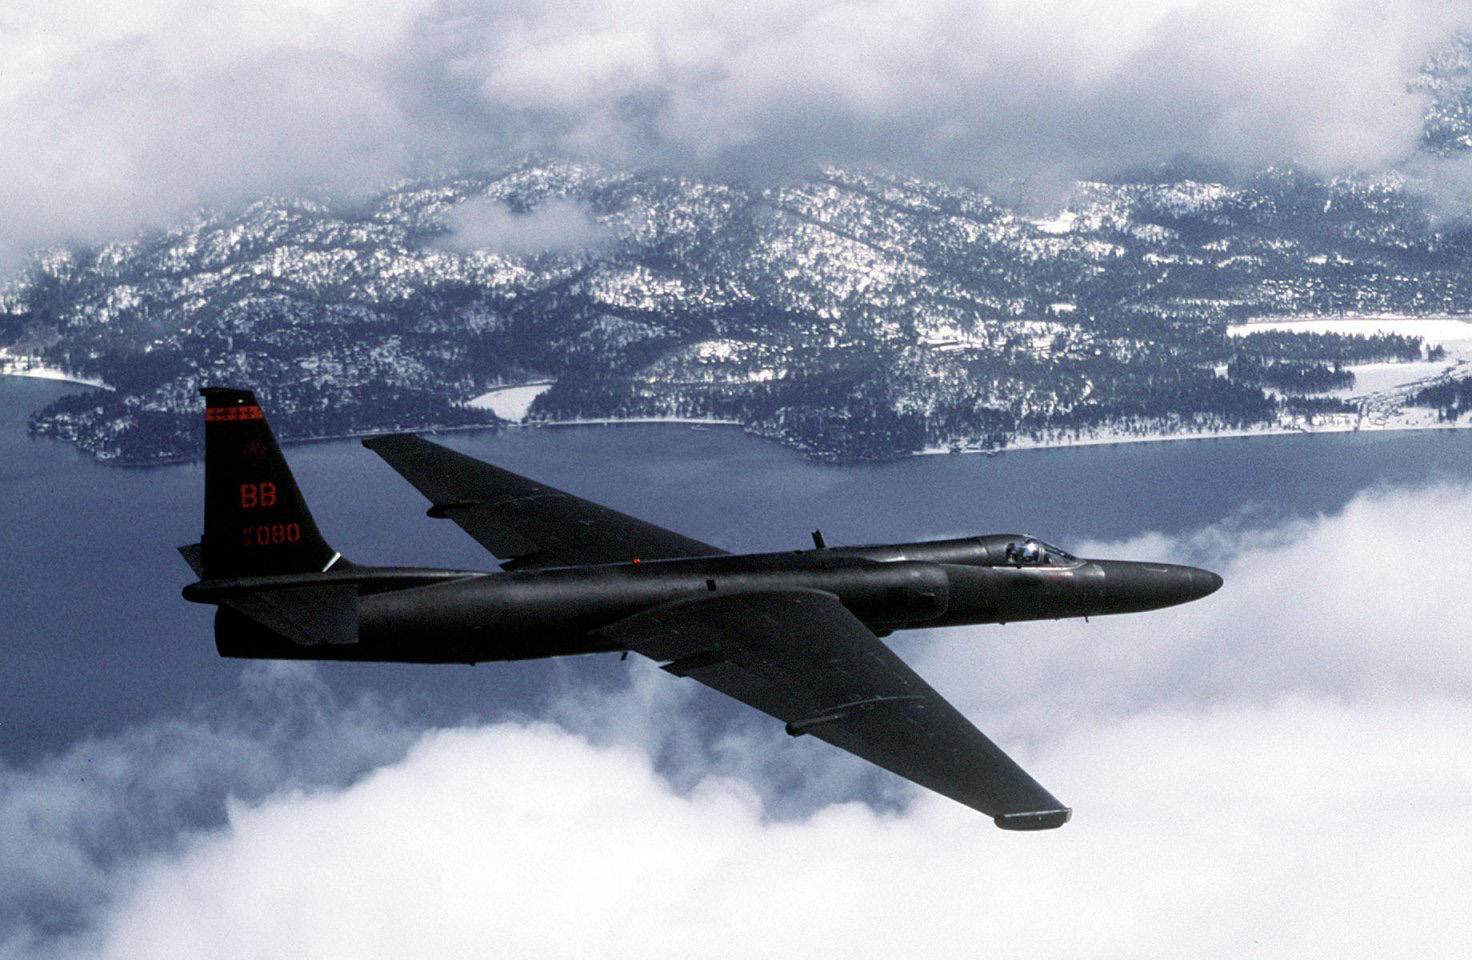
\includegraphics[width=0.6\textwidth]{figures/US_Air_Force_U-2_reconnaissance_aircraft_H.jpg}
    \caption{US Air Force reconnaissance aircraft during the First World War. Credit: US Air Force.}
\end{figure}

\column{0.45\textwidth}

\begin{figure}
    \center
    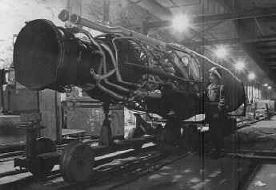
\includegraphics[width=0.5\textwidth]{figures/Dora_-_production.jpeg}
    \caption{The V2 missile assembly line in the Mittelwerk complex at the Dora concentration camp. Credit: User Ericd on en.wikipedia — US Army signal corps.}
\end{figure}

\end{columns}

\end{frame}
%---------------------------------------------------------------------------
\begin{frame}{The beginning of the space race\footnote{\url{https://fr.wikipedia.org\/wiki\/Satellite\_artificiel}}}

\begin{itemize}[label=$\blacktriangleright$]
    \item \textbf{1957} Launch of the first artificial Earth satellite, Sputnik 1, by the USSR,
    \item \textbf{1958} Creation of the National Aeronautics and Space Administration (NASA) at the initiative of President Eisenhower, and launch of the first American satellite, Explorer 1.
    \item \textbf{1962} Creation of the Centre National d'Etudes Spatiales (CNES, French National Centre for Space Studies) at the initiative of General de Gaulle,
    \item \textbf{1965} Launch of the first French satellite, Astérix, with the Diamant A rocket. France becomes the third power to achieve an orbital launch with a national launcher.
\end{itemize}

\begin{figure}
    \center
    \begin{subfigure}{0.3\textwidth}
        \center
        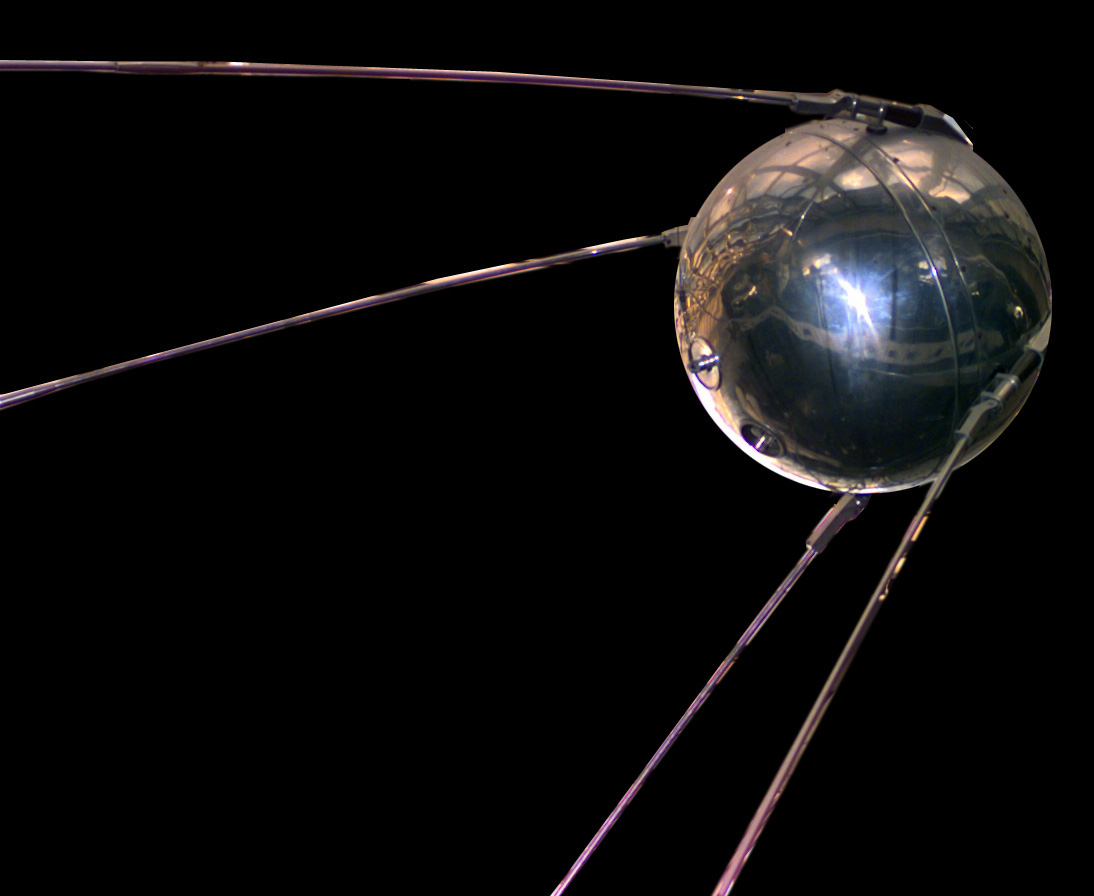
\includegraphics[width=0.85\textwidth]{figures/Sputnik_asm.jpeg
}
        \caption{Replica of Sputnik 1, National Air and Space Museum.}
    \end{subfigure}
    \begin{subfigure}{0.3\textwidth}
        \center
        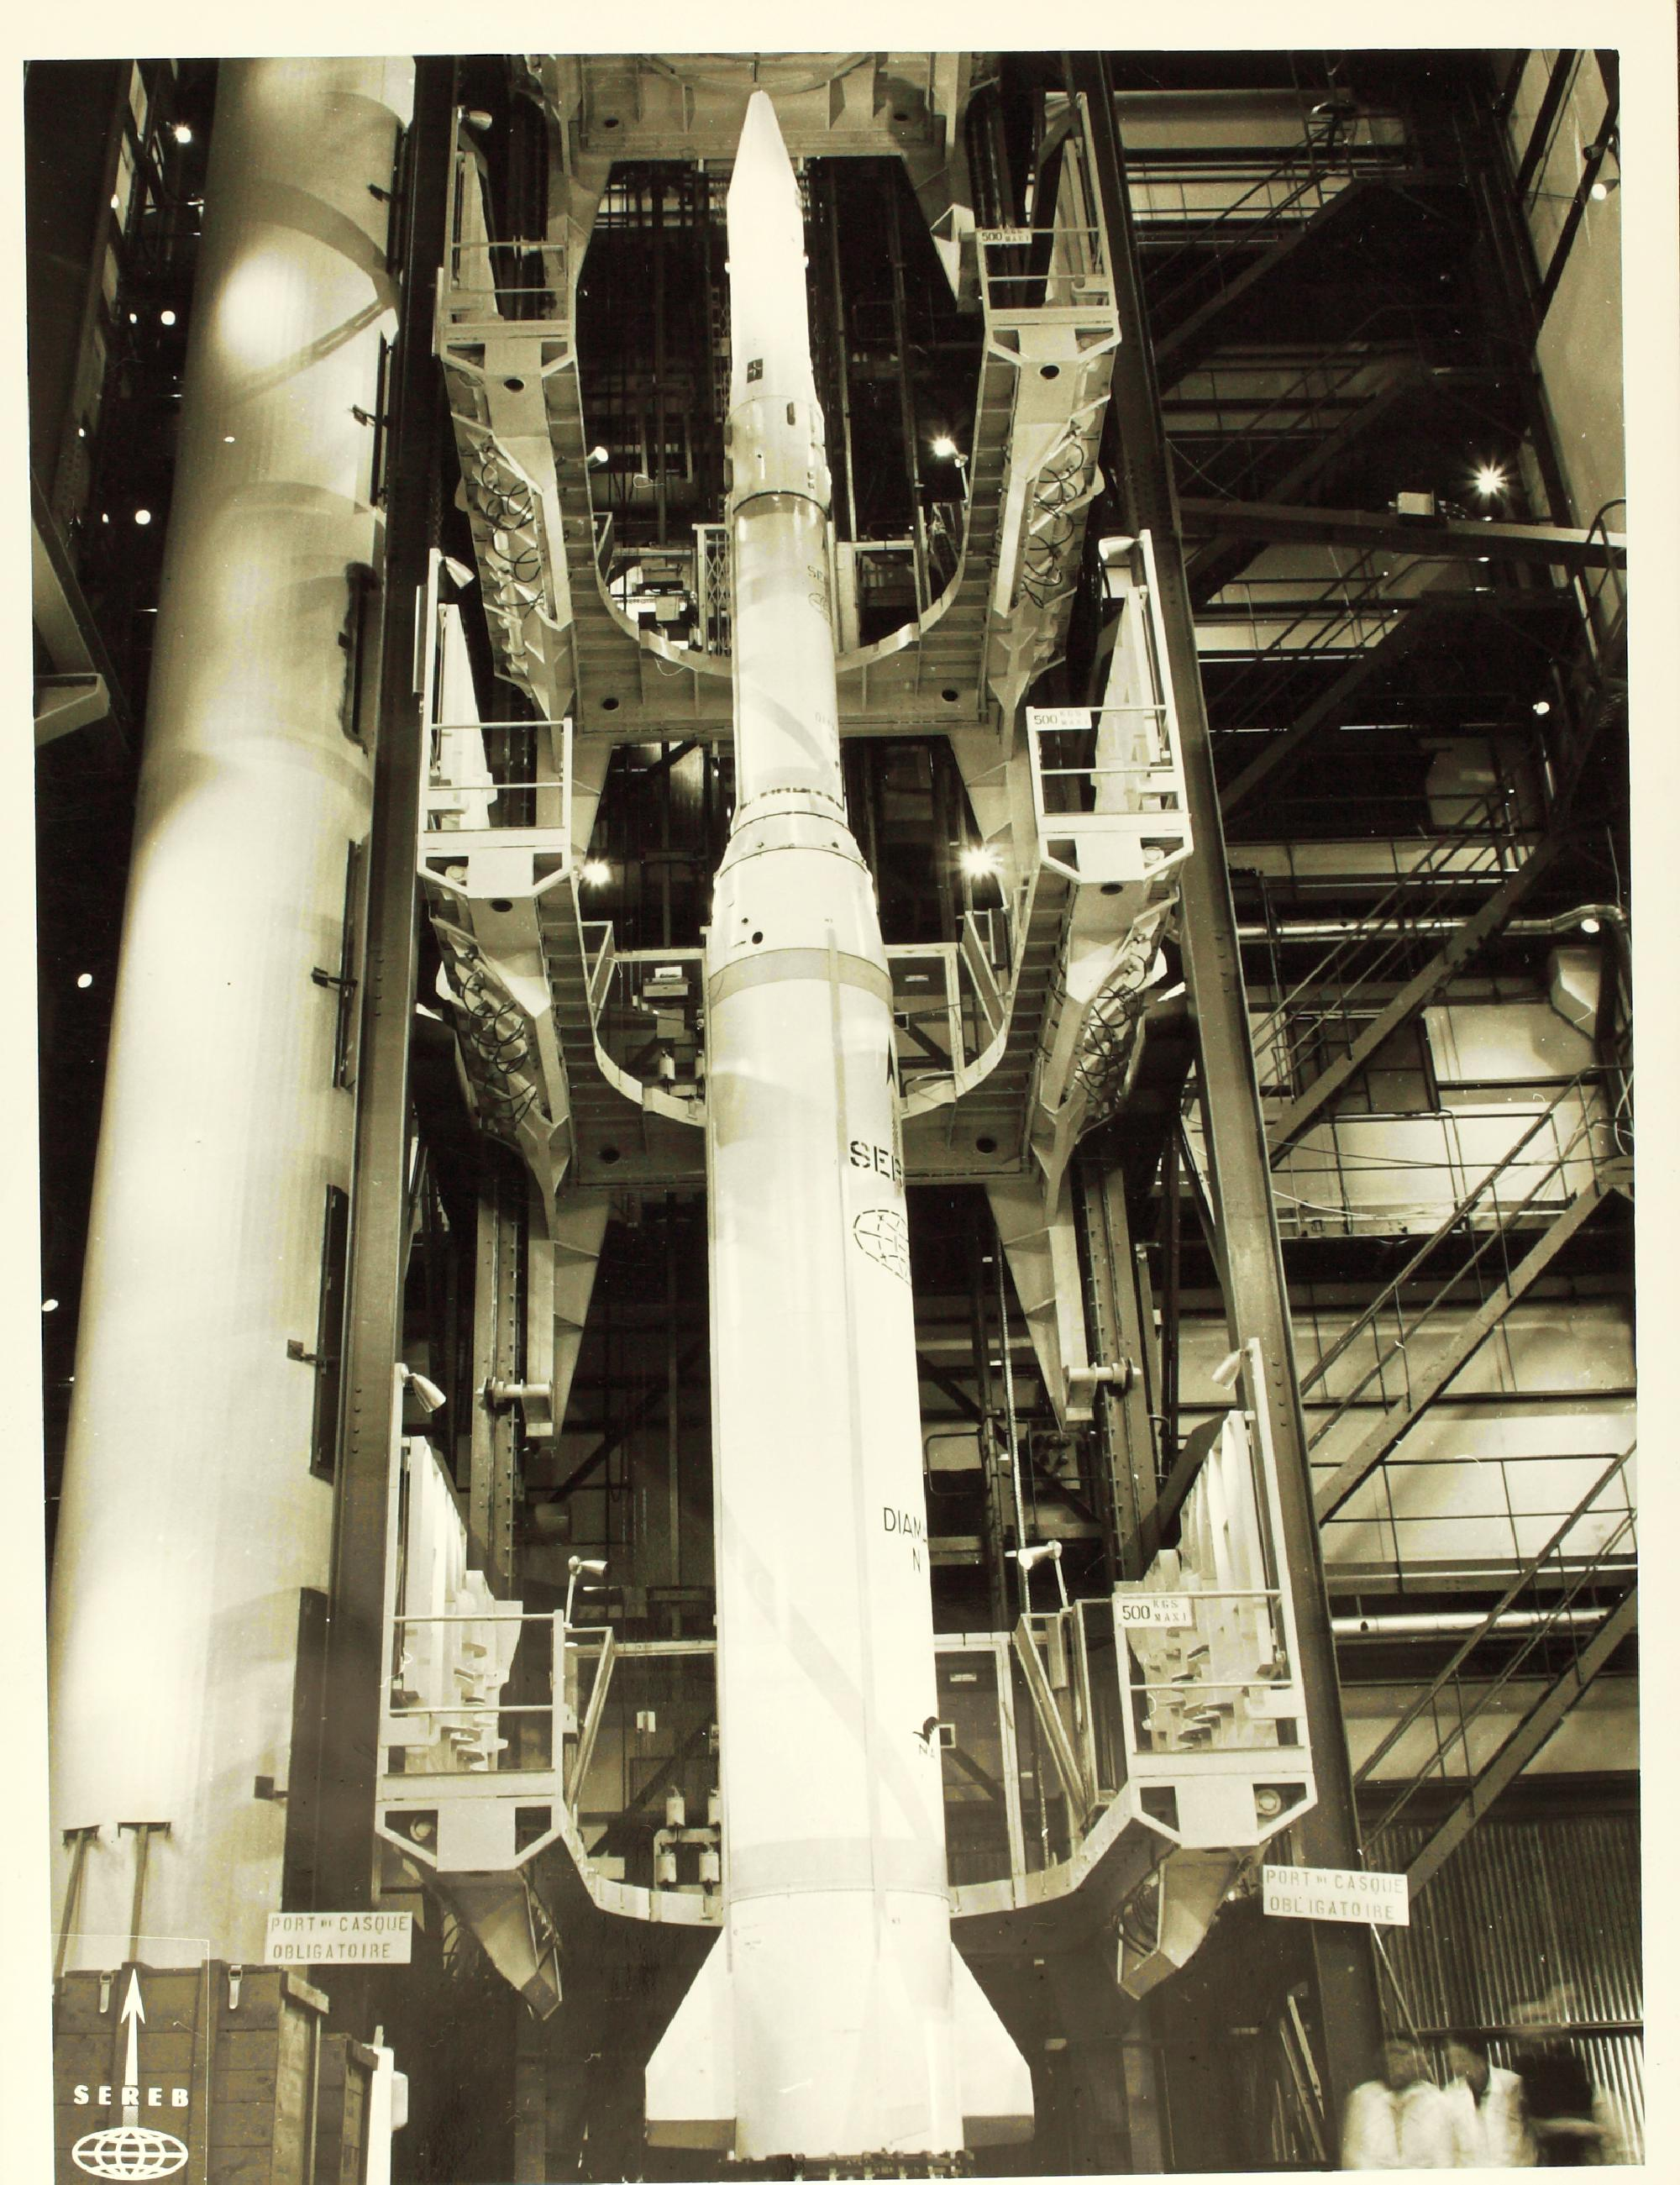
\includegraphics[width=0.55\textwidth]{figures/Diamant_A.jpeg}
        \caption{Diamant A rocket in its assembly building.}
    \end{subfigure}
    \begin{subfigure}{0.3\textwidth}
        \center
        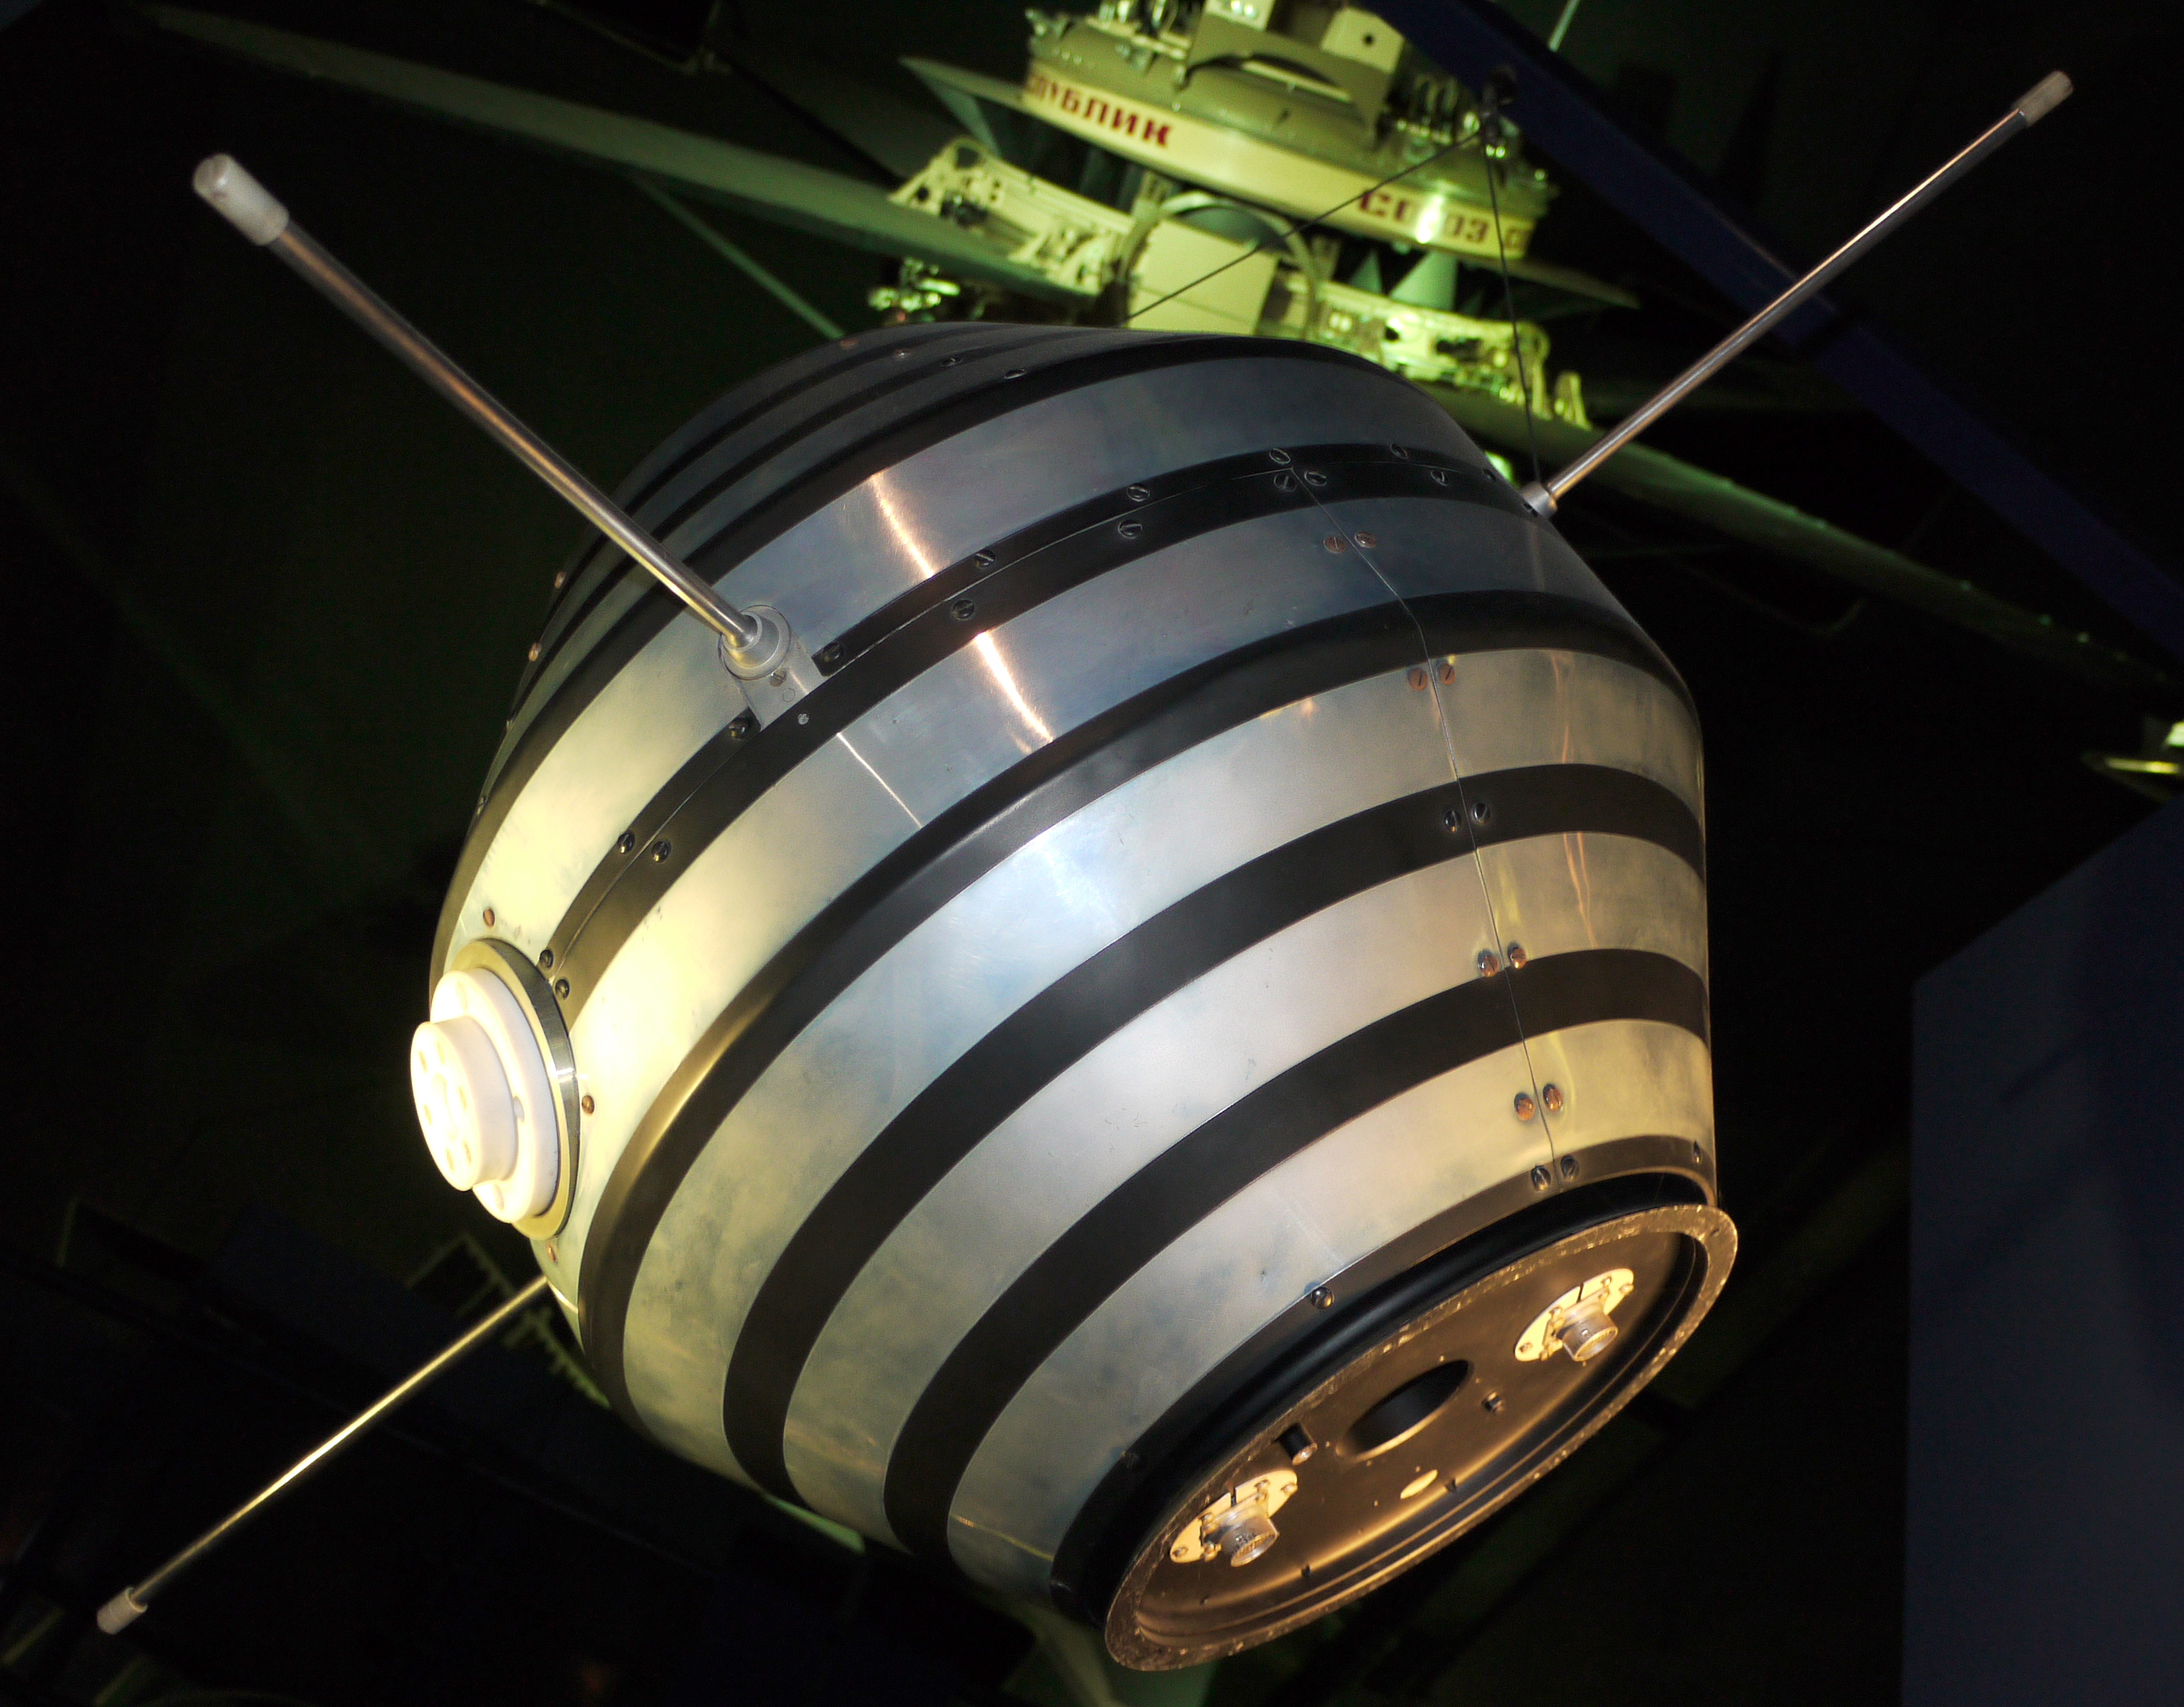
\includegraphics[width=0.9\textwidth]{figures/Asterix_Musee_du_Bourget_P1020341.jpeg
}
        \caption{Replica of Astérix, Musée de l'Air et de l'Espace, Paris Le Bourget.}
    \end{subfigure}
\end{figure}

\end{frame}
%---------------------------------------------------------------------------
\begin{frame}{First Earth observation satellites: weather satellites}

\begin{itemize}[label=$\blacktriangleright$]
    \item \textbf{1960} Launch of the first weather satellite TIROS-1 by NASA,
    \item \textbf{1964} Launch of the Meteor-1 weather satellite by the USSR,
    \item \textbf{1977} Launch of the European weather satellite Meteosat-1 by ESA (European Space Agency).
\end{itemize}

\begin{columns}

\column{0.45\textwidth}

\begin{figure}
    \center
    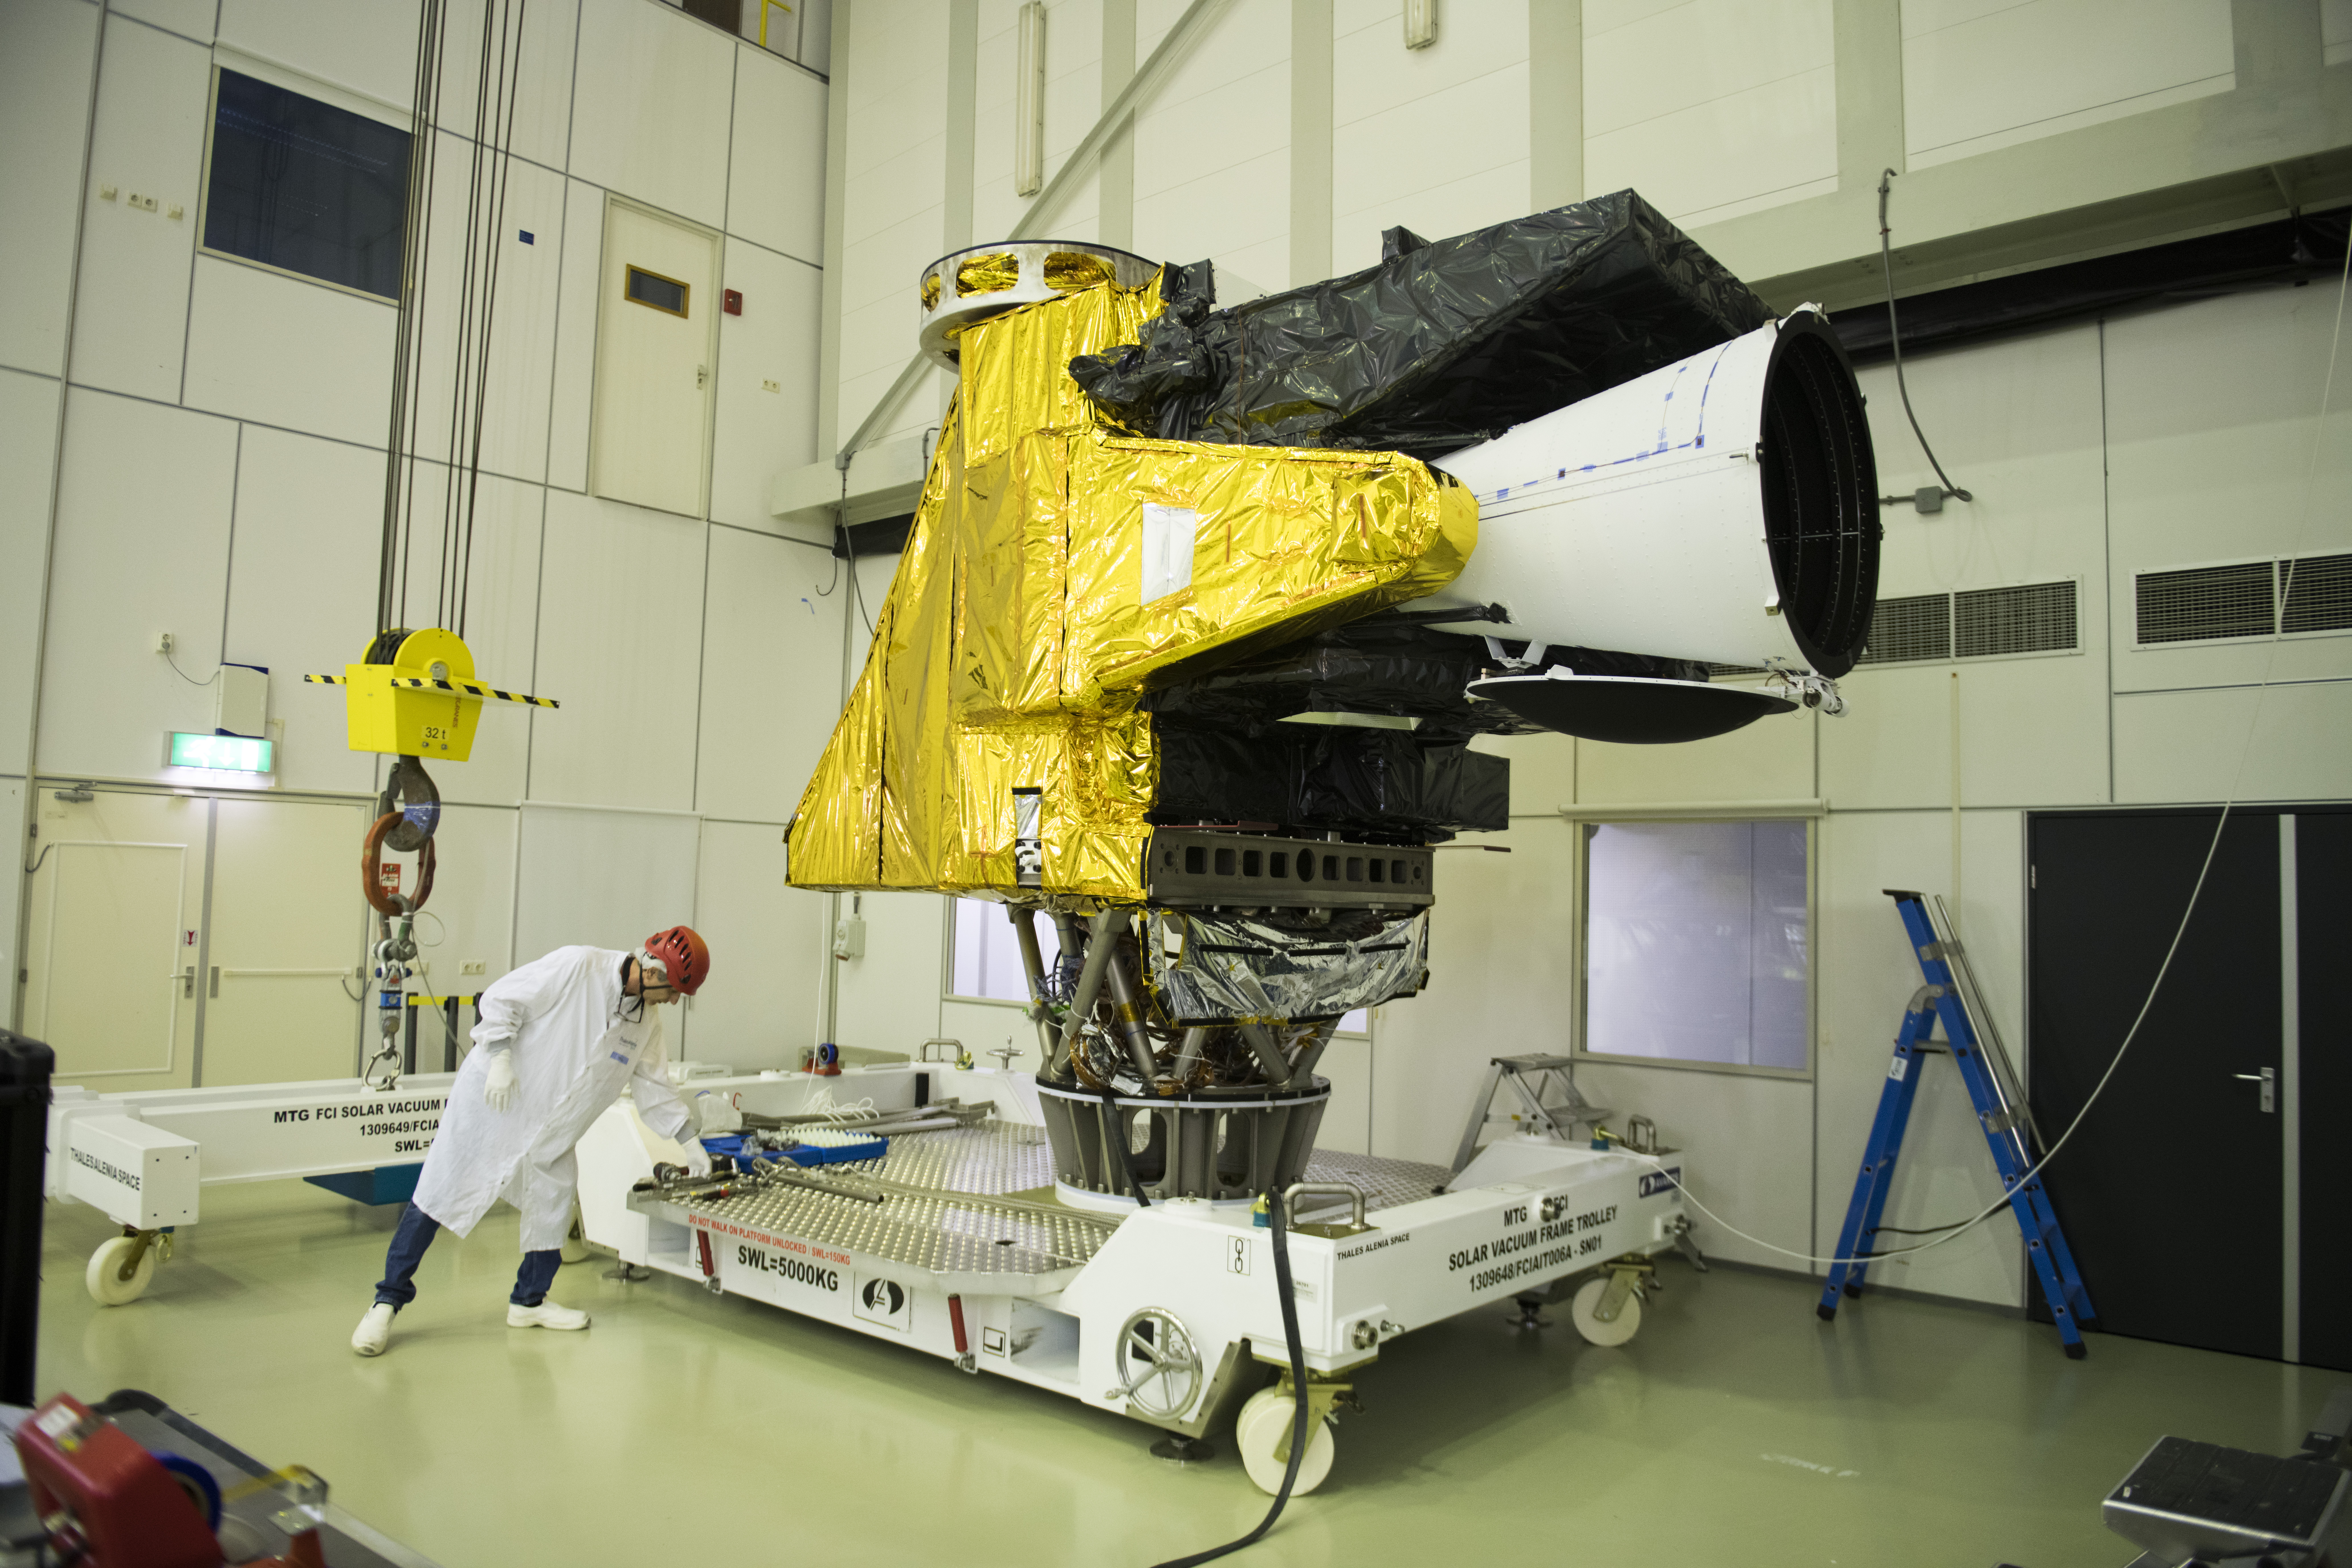
\includegraphics[width=0.7\textwidth]{figures/FCI_at_Test_Centre_ESA396236.jpeg}
    \caption{FCI imager radiometer of the European geostationary weather satellite MTG (third-generation Meteosat). Credit: ESA.}
\end{figure}

\column{0.45\textwidth}

\begin{figure}
    \center
    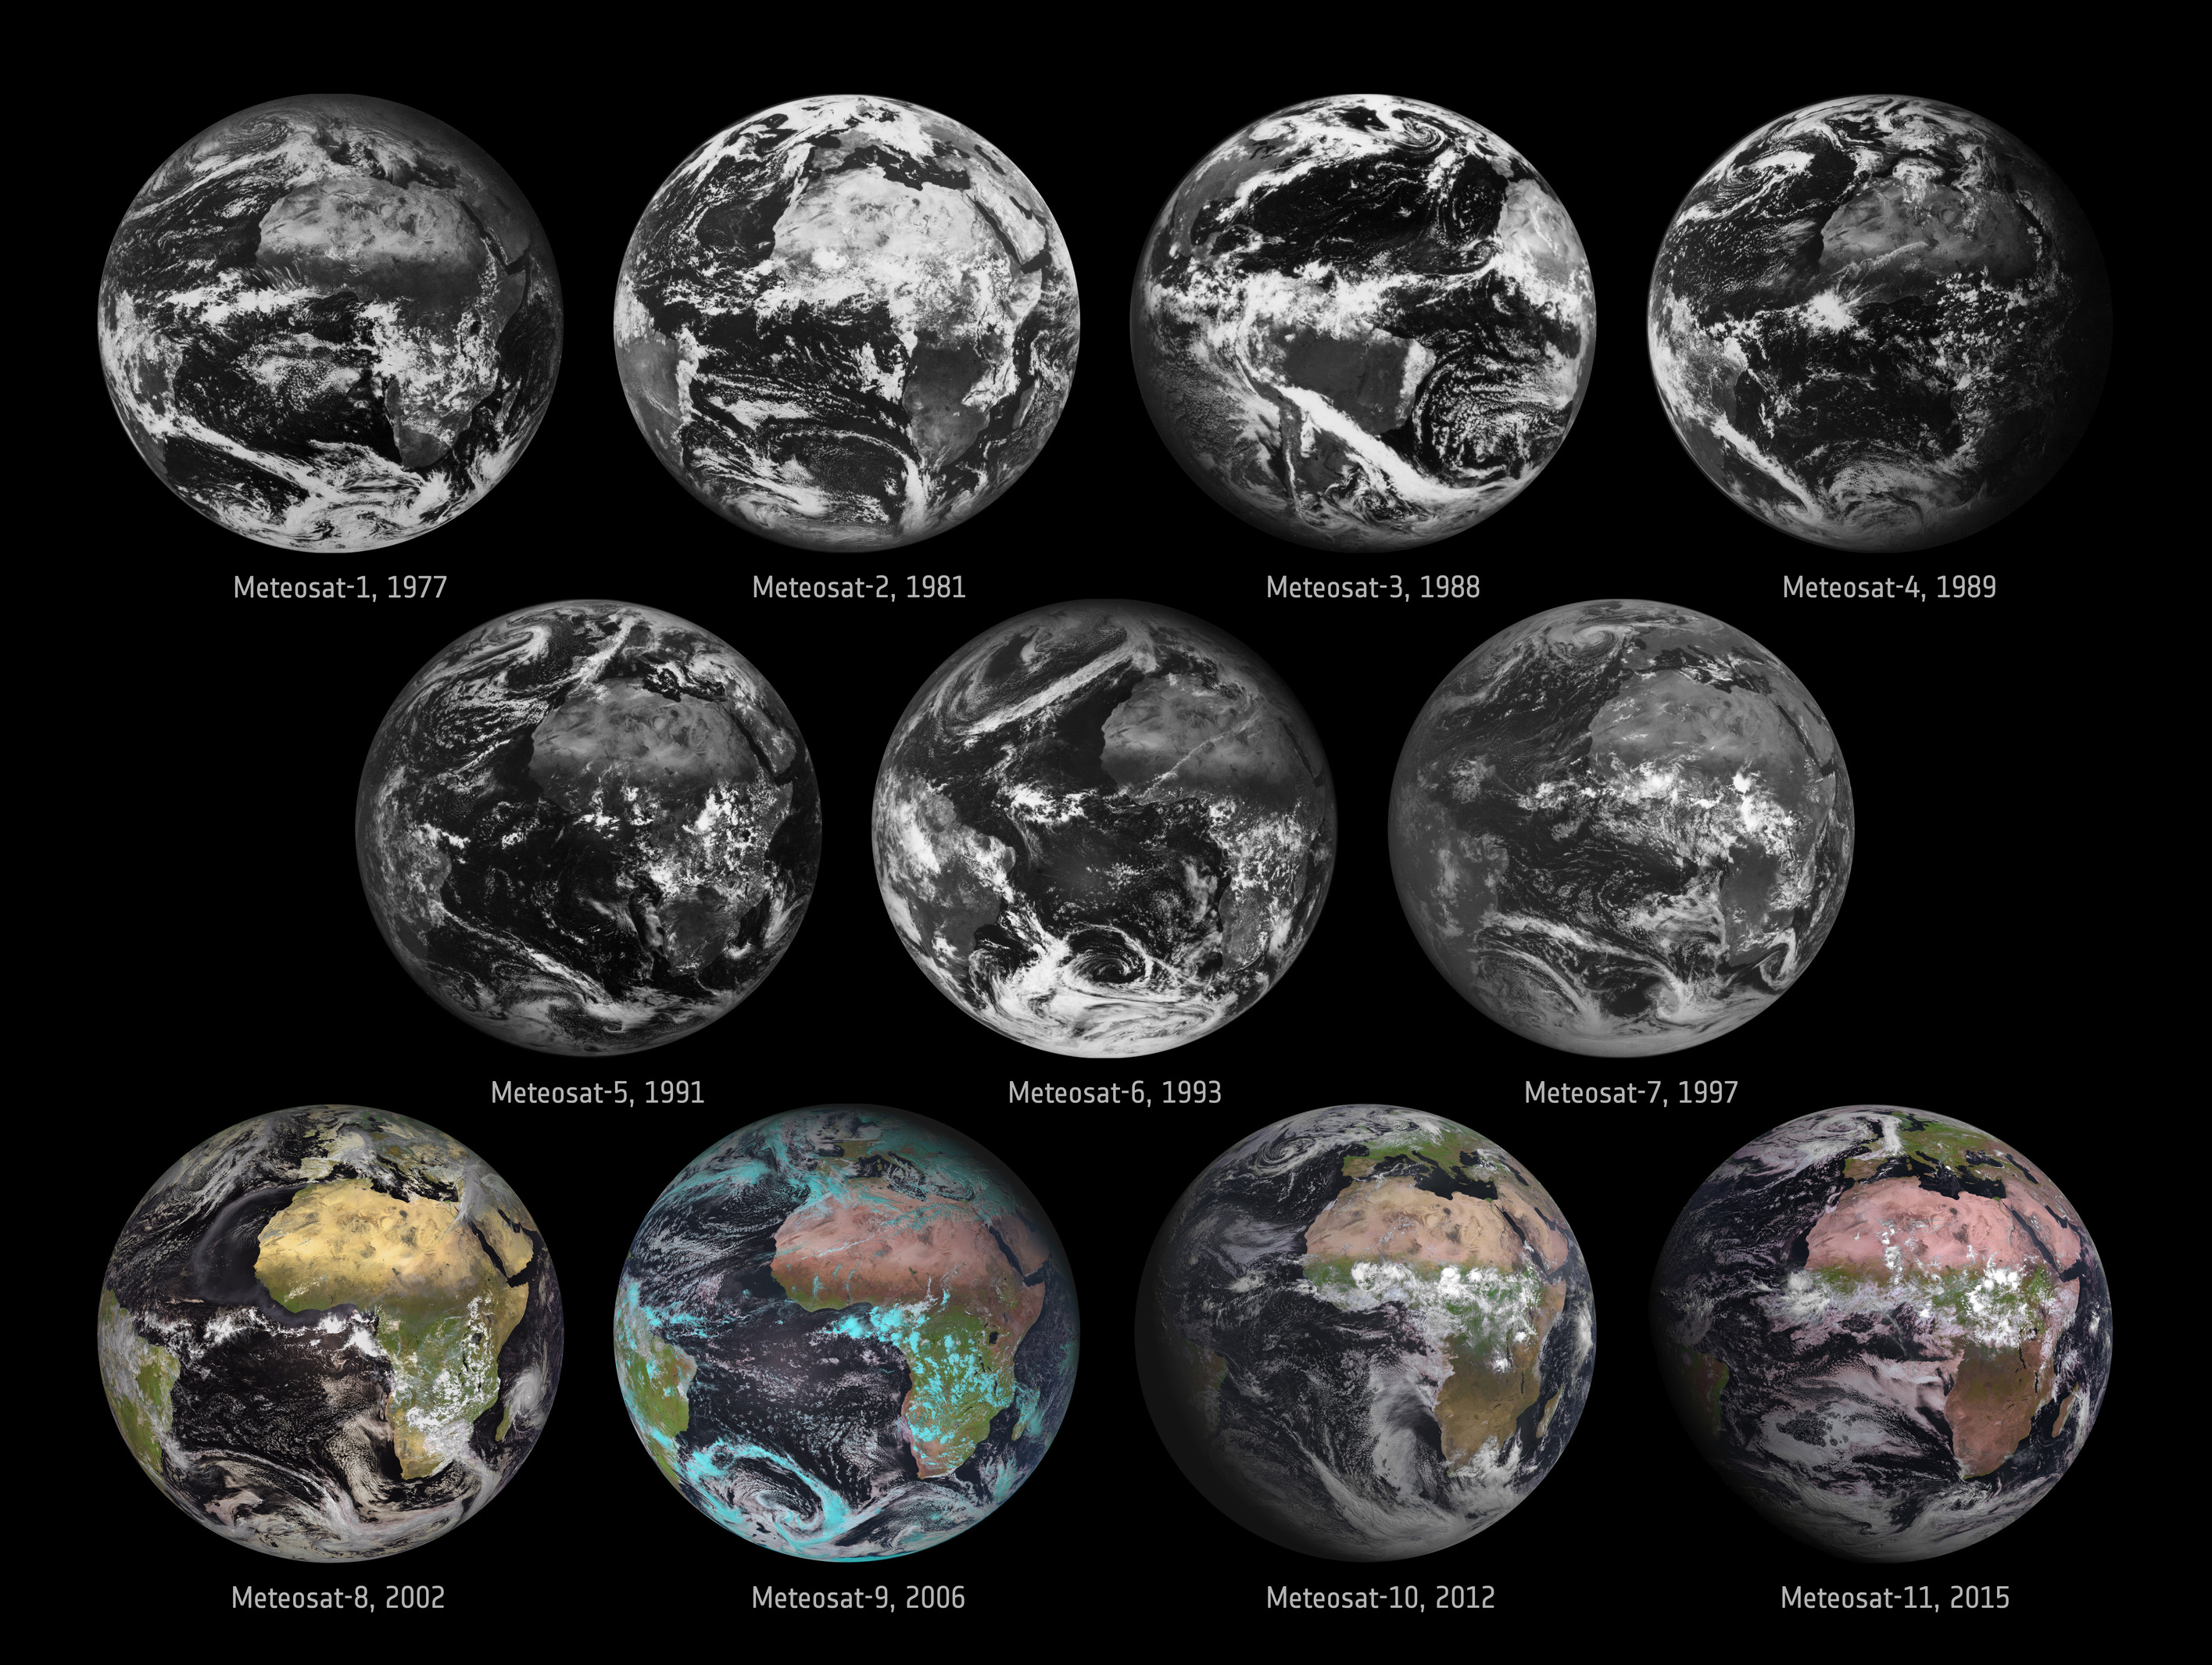
\includegraphics[width=0.65\textwidth]{figures/Meteosat_first_images.jpg}
    \caption{Color composites of images from the first- and second-generation Meteosat satellites. Credit: ESA/Eumetsat.}
\end{figure}

\end{columns}

\end{frame}
%---------------------------------------------------------------------------
\begin{frame}{First civilian satellites for observing land surfaces}

\begin{itemize}[label=$\blacktriangleright$]
    \item \textbf{1972} Launch of the first land observation satellite, Landsat, by NASA, at the instigation of the United States Geological Survey and the Department of Agriculture,
    \item \textbf{1986} Launch of the competing SPOT satellite by CNES. In 2021, CNES released an archive of 19 million SPOT images acquired between 1986 and 2015.
    %\item \textbf{2015} Launch of Sentinel-2 by ESA as part of the Copernicus programme. The acquired images are freely accessible.
\end{itemize}

\begin{columns}

\column{0.25\textwidth}

\begin{figure}
    \center
    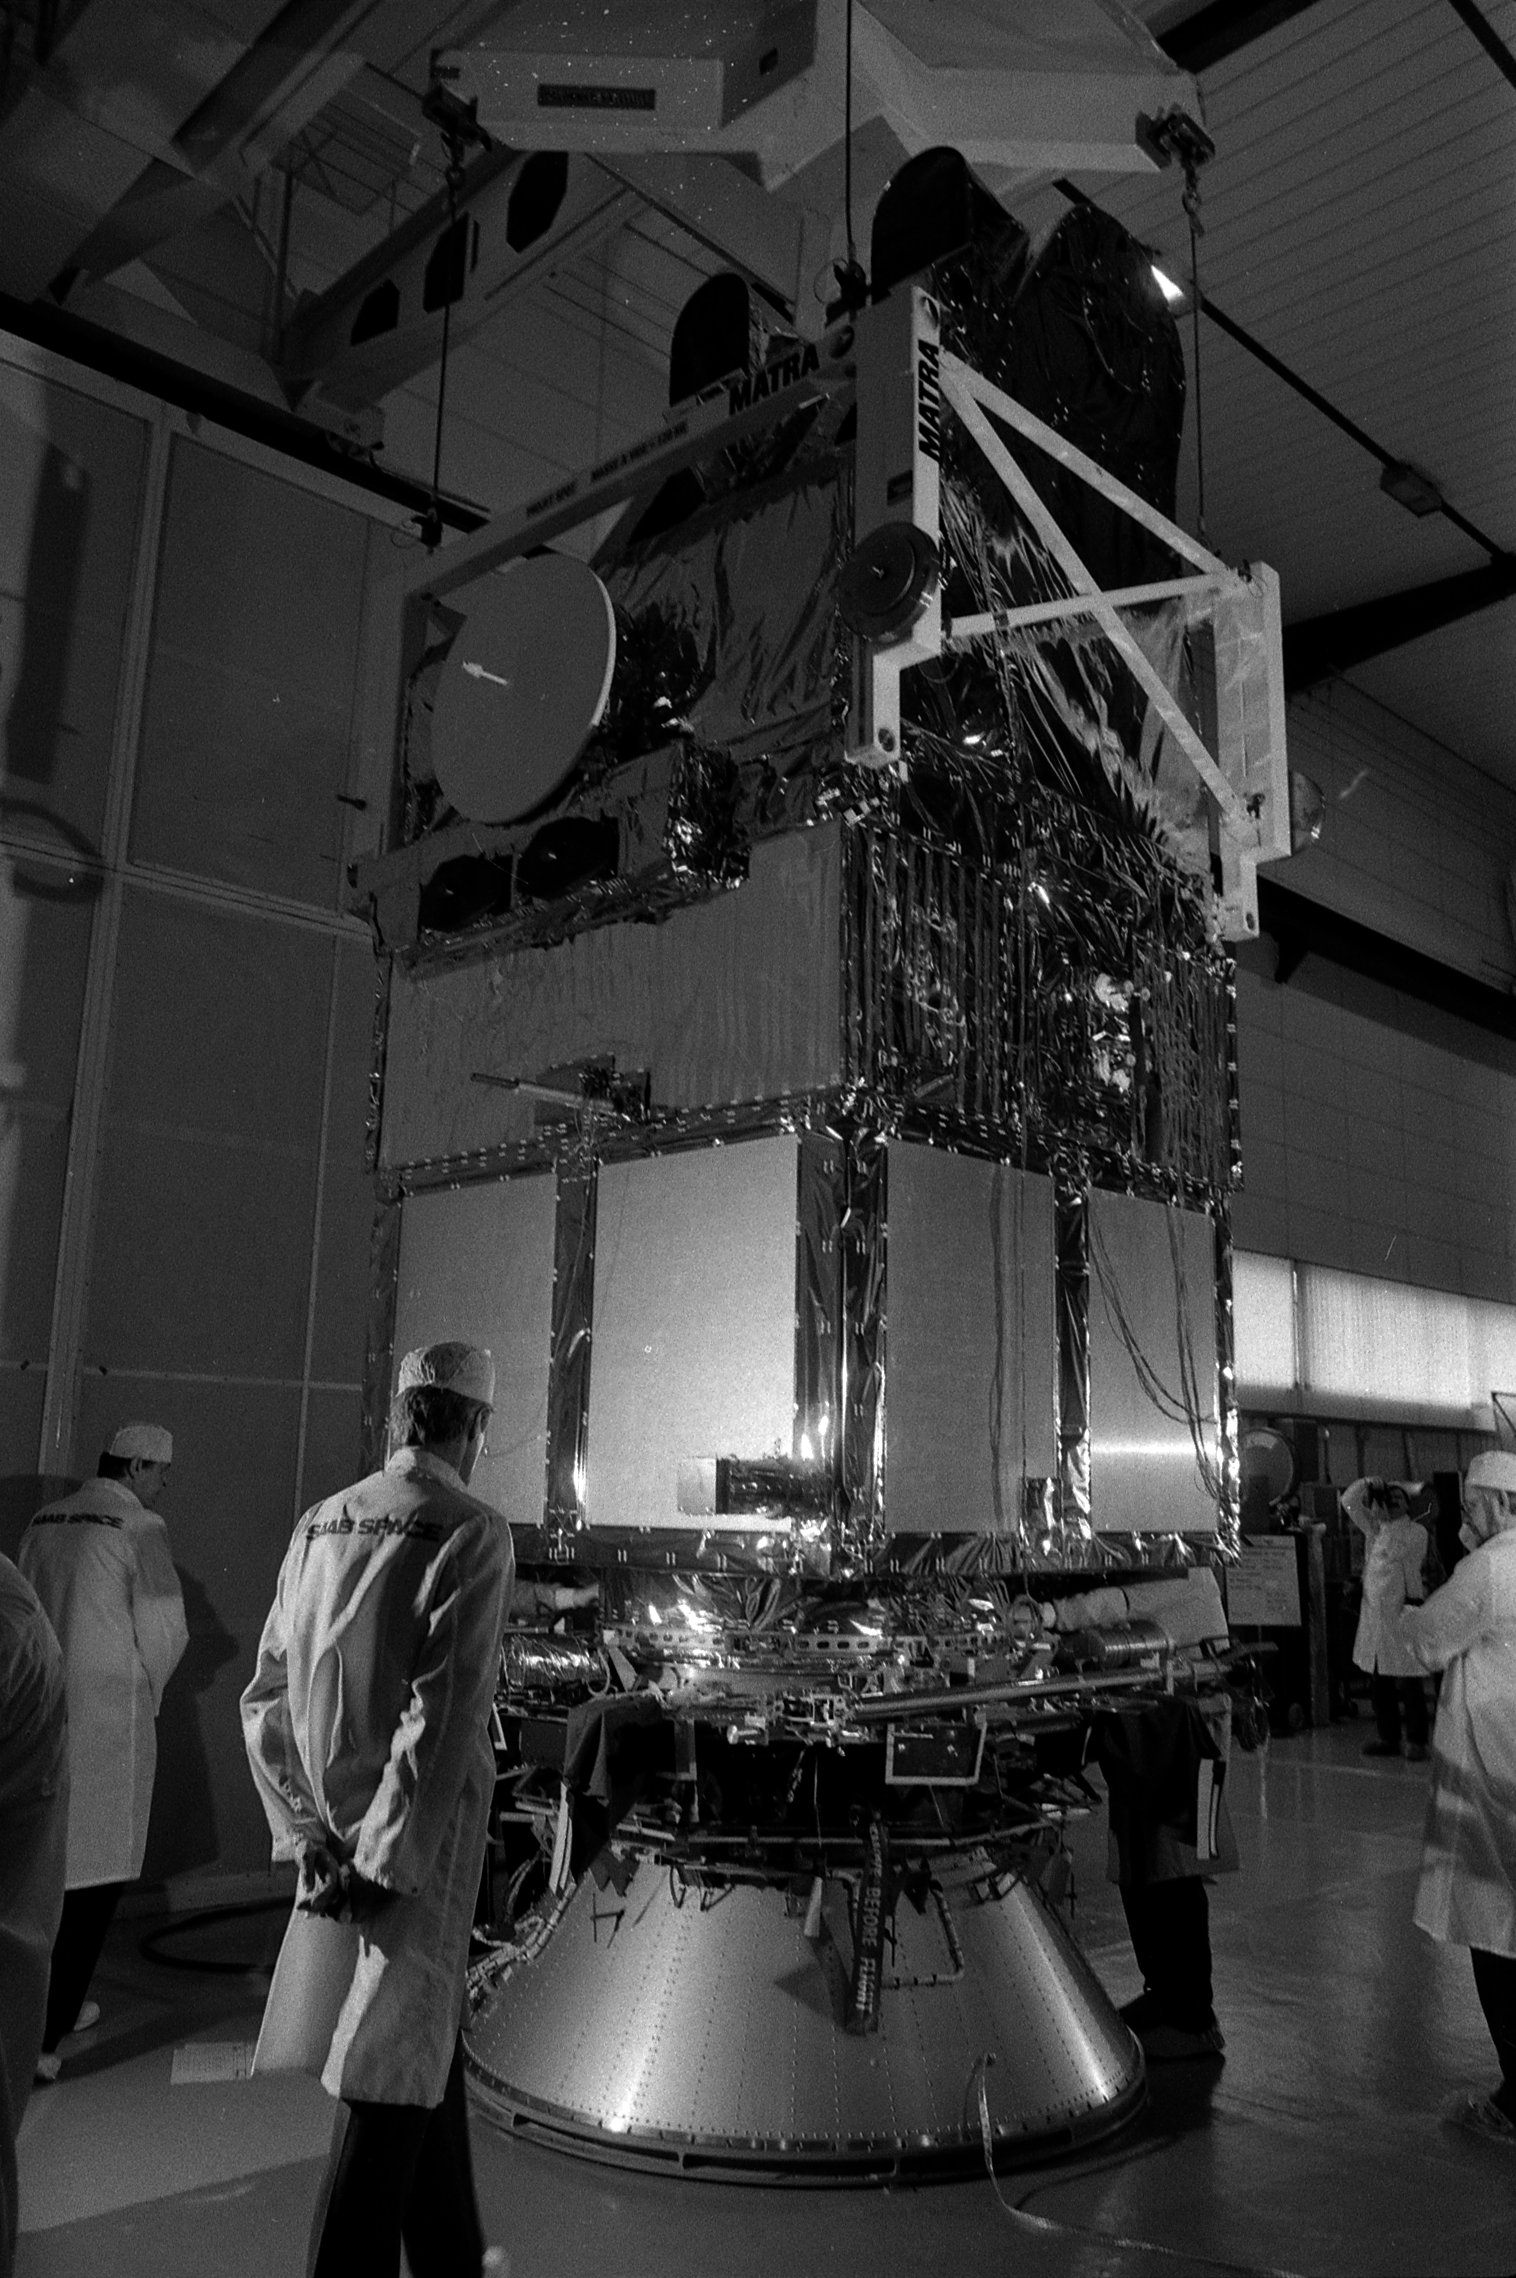
\includegraphics[width=0.5\textwidth]{figures/11.03.85_Au_CNES_satellite_Spot_1_(1985)_-_53Fi2121.jpeg
}
    \caption{Presentation of SPOT-1 at the Toulouse Space Centre on 11 March 1985. Credit: André Cros.}
\end{figure}

\column{0.25\textwidth}

\begin{figure}
    \center
    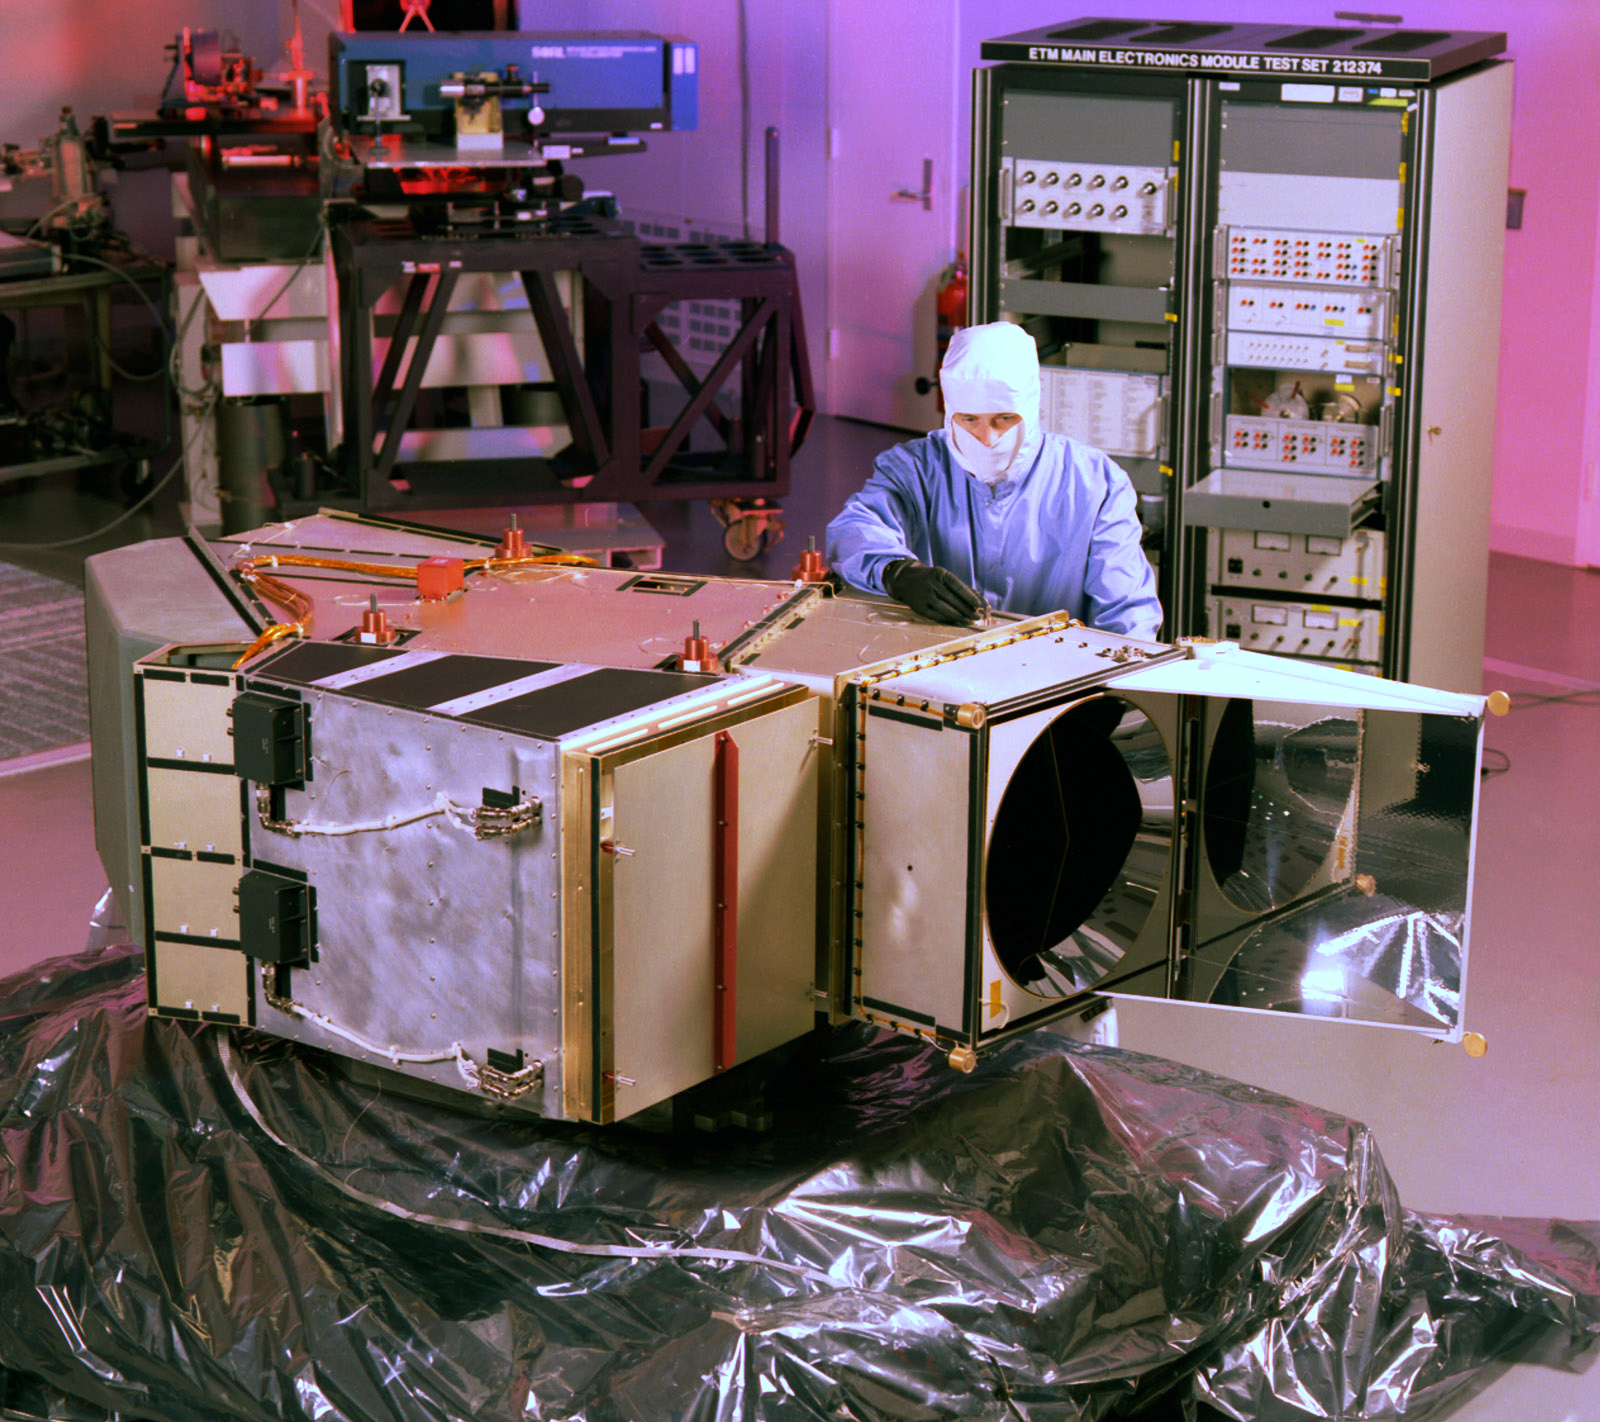
\includegraphics[width=0.9\textwidth]{figures/Landsat_7_ETM_instrument.jpeg}
    \caption{The ETM+ instrument of Landsat 7. Credit: NASA.}
\end{figure}

\column{0.25\textwidth}

\begin{figure}
    \center
    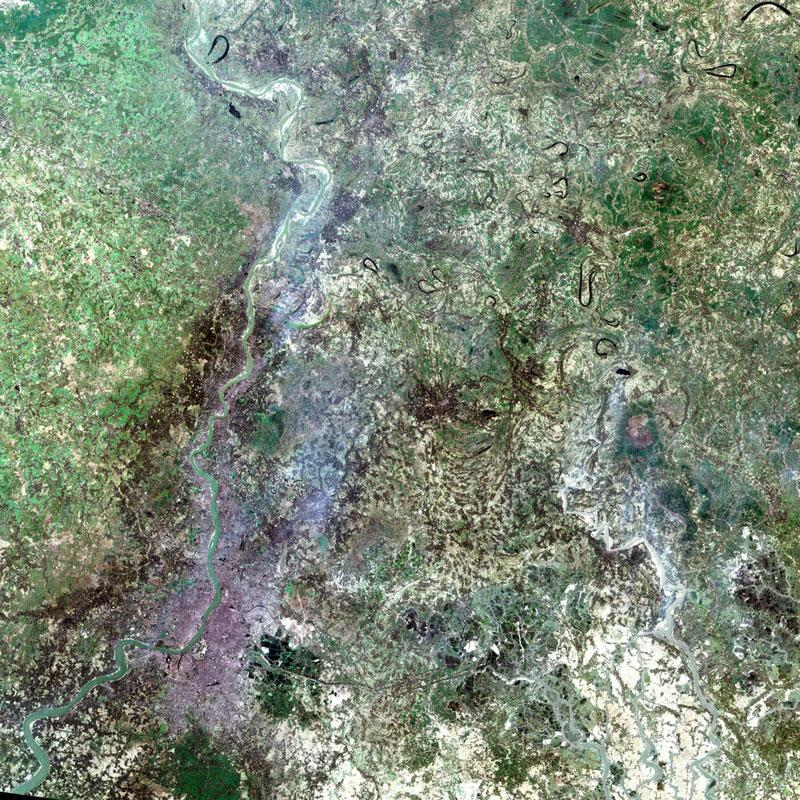
\includegraphics[width=0.8\textwidth]{figures/Large_Kolkata_Landsat.jpeg}
    \caption{Color composite of a Landsat 7 image of Kolkata (India). Credit: NASA.}
\end{figure}

\end{columns}

\end{frame}
%---------------------------------------------------------------------------
\subsection{Principles of optical remote sensing}
%---------------------------------------------------------------------------
\begin{frame}{Outline}
\tableofcontents[currentsection, currentsubsection]
\end{frame}
%---------------------------------------------------------------------------
\begin{frame}{Passive and Active Remote Sensing}

Classification of the different types of remote sensing
\begin{itemize}[label=$\blacktriangleright$]
    \item \textbf{Passive solar remote sensing}: measurement of solar radiation reflected by the Earth, \textit{e.g.} from visible to shortwave infrared (0.4 µm - 2.5 µm),
    \item \textbf{Passive thermal remote sensing}: measurement of thermal radiation emitted by the Earth, \textit{e.g.} in the thermal infrared (3 - 15 µm), or in the microwaves (220 MHz - 40 GHz).
    \item \textbf{Active remote sensing}: emission of lidar (visible, infrared) or radar (microwave) radiation and measurement of the backscattered radiation (\textit{e.g.} altimeter, SAR).
\end{itemize}

\begin{figure}
	\center
	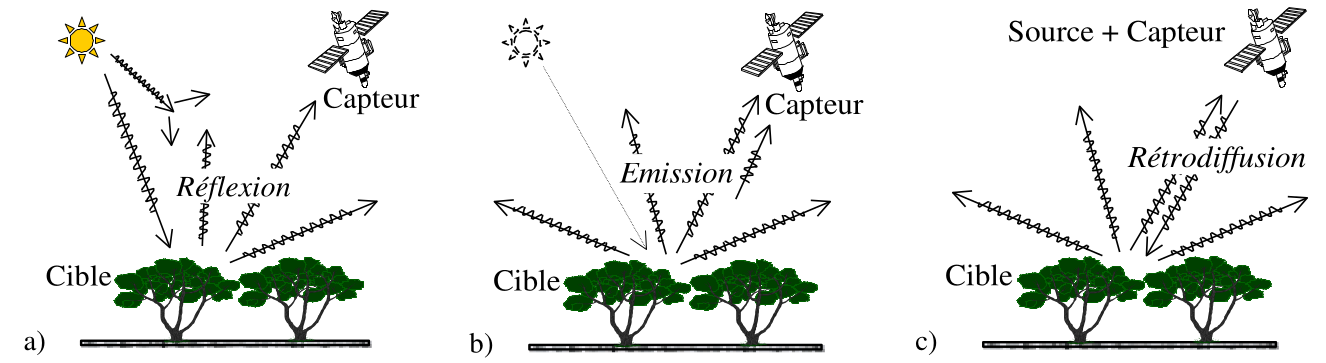
\includegraphics[width=0.7\textwidth]{figures/cat_teledec.png}
	\caption{a) Passive solar, b) passive thermal, c) active. Credit: J.P. Gastellu-Etchegorry}
\end{figure}

%\begin{figure}
%	\center
%	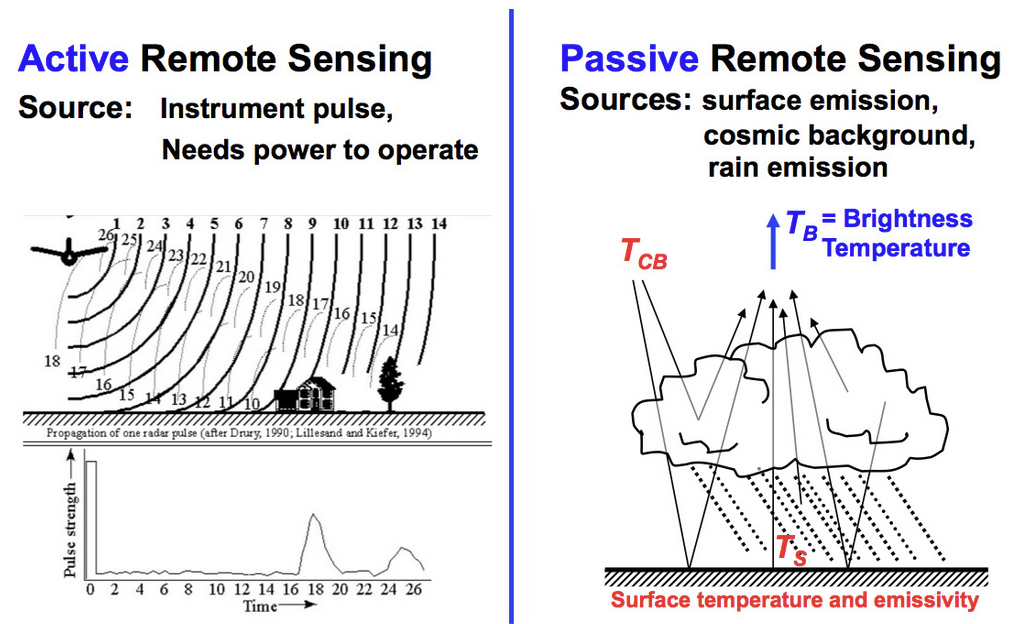
\includegraphics[width=0.5\textwidth]{figures/active_vs_passive.png}
%	
%	{Source: \url{http://pmm.nasa.gov/image-gallery/active-and-passive-remote-sensing-diagram}}
%\end{figure}

\end{frame}
%---------------------------------------------------------------------------
%\begin{frame}{Remote sensing of forests}
%
%Optical remote sensing provides information on the biochemical properties of vegetation, while active remote sensing provides information on the geometric properties and moisture of vegetation and soils.
%
%\end{frame}
%---------------------------------------------------------------------------
\begin{frame}{Solar radiance}

\begin{figure}
	\center
	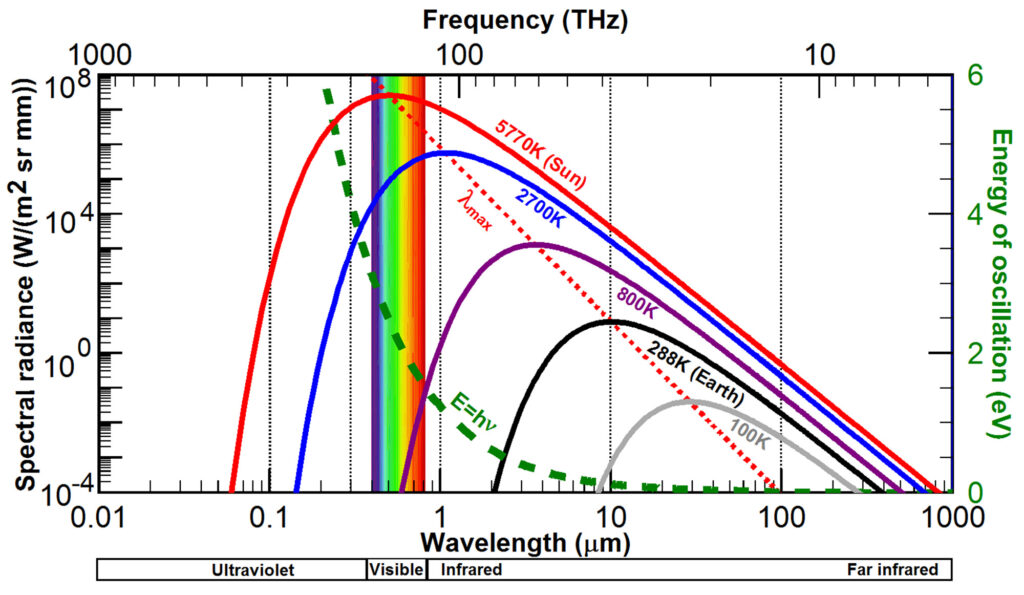
\includegraphics[width=0.7\textwidth]{figures/plancks-law.jpg}
	\caption{Solid lines show the radiation from a black body according to Planck’s law. The red line shows the radiation for the Sun at 5770K; the black line for the Earth at 288K. The dashed red line connects the peak spectral radiances ($\lambda_{max}$) for each temperature, a consequence of Wien’s displacement law. The dashed green line shows the energy ($E=h \nu$) at each wavelength according to Planck’s postulate. Source: \url{ozonedepletiontheory.info/ImagePages/electromagnetic-spectrum/}}
\end{figure}

\end{frame}
%---------------------------------------------------------------------------
\begin{frame}{From solar radiance to top-of-atmosphere irradiance}

\textbf{Radiance} (Luminance in French) is the spectral flux that is emitted or that reaches a surface, per unit of surface, per unit of solid angle, and per unit of wavelength (W/m$^2$/sr/µm). \vspace{0.3cm}


The total flux emitted by the sun is the radiance integrated over the sun surface, over the entire sphere, and over the entire electromagnetic spectrum. \vspace{0.3cm}

\textbf{Irradiance} (Eclairement in French) is the flux that reaches a surface, per surface unit and per wavelength unit (W/m$^2$/µm). \vspace{0.2cm}

\begin{figure}
	\center
	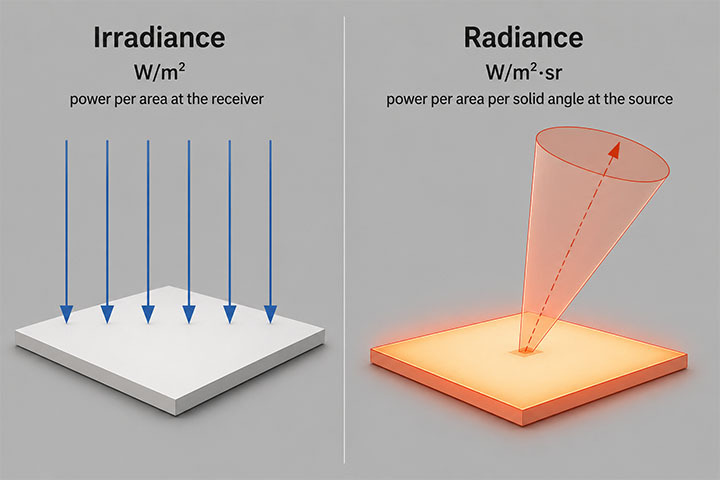
\includegraphics[width=0.3\textwidth]{figures/rad_vs_irr.jpg}
	\caption{Illustration of radiance VS irradiance. Source: \url{https://www.reddotled.com/what-is-the-irradiance-of-light.html}}
\end{figure}

$\blacktriangleright$ \textit{What is the solar irradiance at the top of the atmosphere for a surface orthogonal to the sun direction?} 

\end{frame}
%---------------------------------------------------------------------------
\begin{frame}{Solid angle}

%\begin{columns}

%\column{0.45\textwidth}

The solid angle is a generalization of the notion of angle in a 3D space. Given a point of view and a surface, it is defined as the ratio of the area of the surface projected on a sphere to the square of the sphere's radius:
\begin{align*}
\Omega = S /r^2 
\end{align*}

The solid angle is expressed in steradians (sr), which are m$^2$/m$^2$. An elementary solid angle in spherical coordinates is defined as:
\begin{align*}
	d^2\Omega = \frac{d^2S}{r^2} = \text{sin } \theta \: \text{d}\phi \:  \text{d}\theta
\end{align*}

\begin{figure}
	\center
	\begin{subfigure}{0.45\textwidth}
		\center
		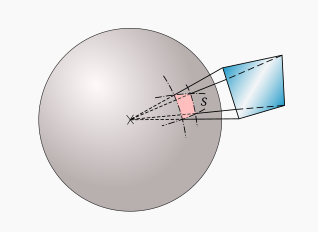
\includegraphics[width=0.5\textwidth]{figures/angle_solide.png}
	\caption{Surface bounded by the projection of a planar quadrilateral onto a sphere, defining the solid angle. Copyright © Christophe Dang Ngoc Chan}
	\end{subfigure}
	\begin{subfigure}{0.45\textwidth}
		\center
		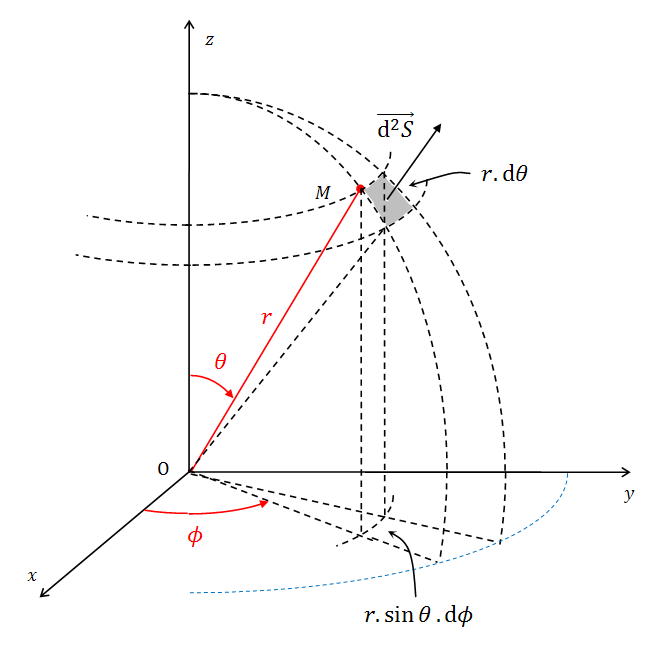
\includegraphics[width=0.5\textwidth]{figures/ds2.png}
	\caption{Illustration of an elementary surface in spherical coordinates. Source: \url{https://fr.wikipedia.org/wiki/Angle_solide}}
	\end{subfigure}
\end{figure}

%\column{0.45\textwidth}


%\end{columns}
\end{frame}
%---------------------------------------------------------------------------
\begin{frame}{Atmosphere transmittance: scattering}

Atmosphere only transmits a fraction of solar irradiance because of absorption and scattering. There are mainly two types of scattering:
\begin{itemize}[label=$\bullet$]
	\item \textbf{Rayleigh} scattering for molecules, proportional to $\lambda^{-4}$,
	\item \textbf{Mie} scattering for bigger particles (\textit{i.e.} aerosols such as dust or cloud droplets): stronger in the forward direction.
\end{itemize}


\begin{figure}
	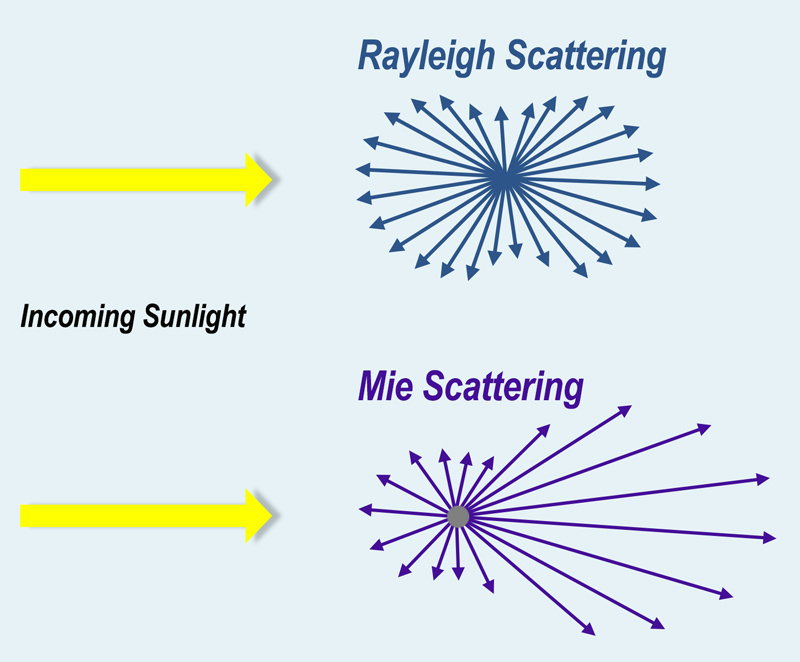
\includegraphics[width=0.3\textwidth]{figures/scattering.jpg}
	\caption{Illustration of Rayleigh and Mie scattering. Source: \url{https://pace.oceansciences.org/prop_of_light.cgi}}
\end{figure}

\end{frame}
%---------------------------------------------------------------------------
\begin{frame}{Atmosphere transmittance: scattering}

$\blacktriangleright$ \textit{What types of scattering are involved in these images?}

\begin{figure}
	\center
	\begin{subfigure}{0.45\textwidth}
		\center
		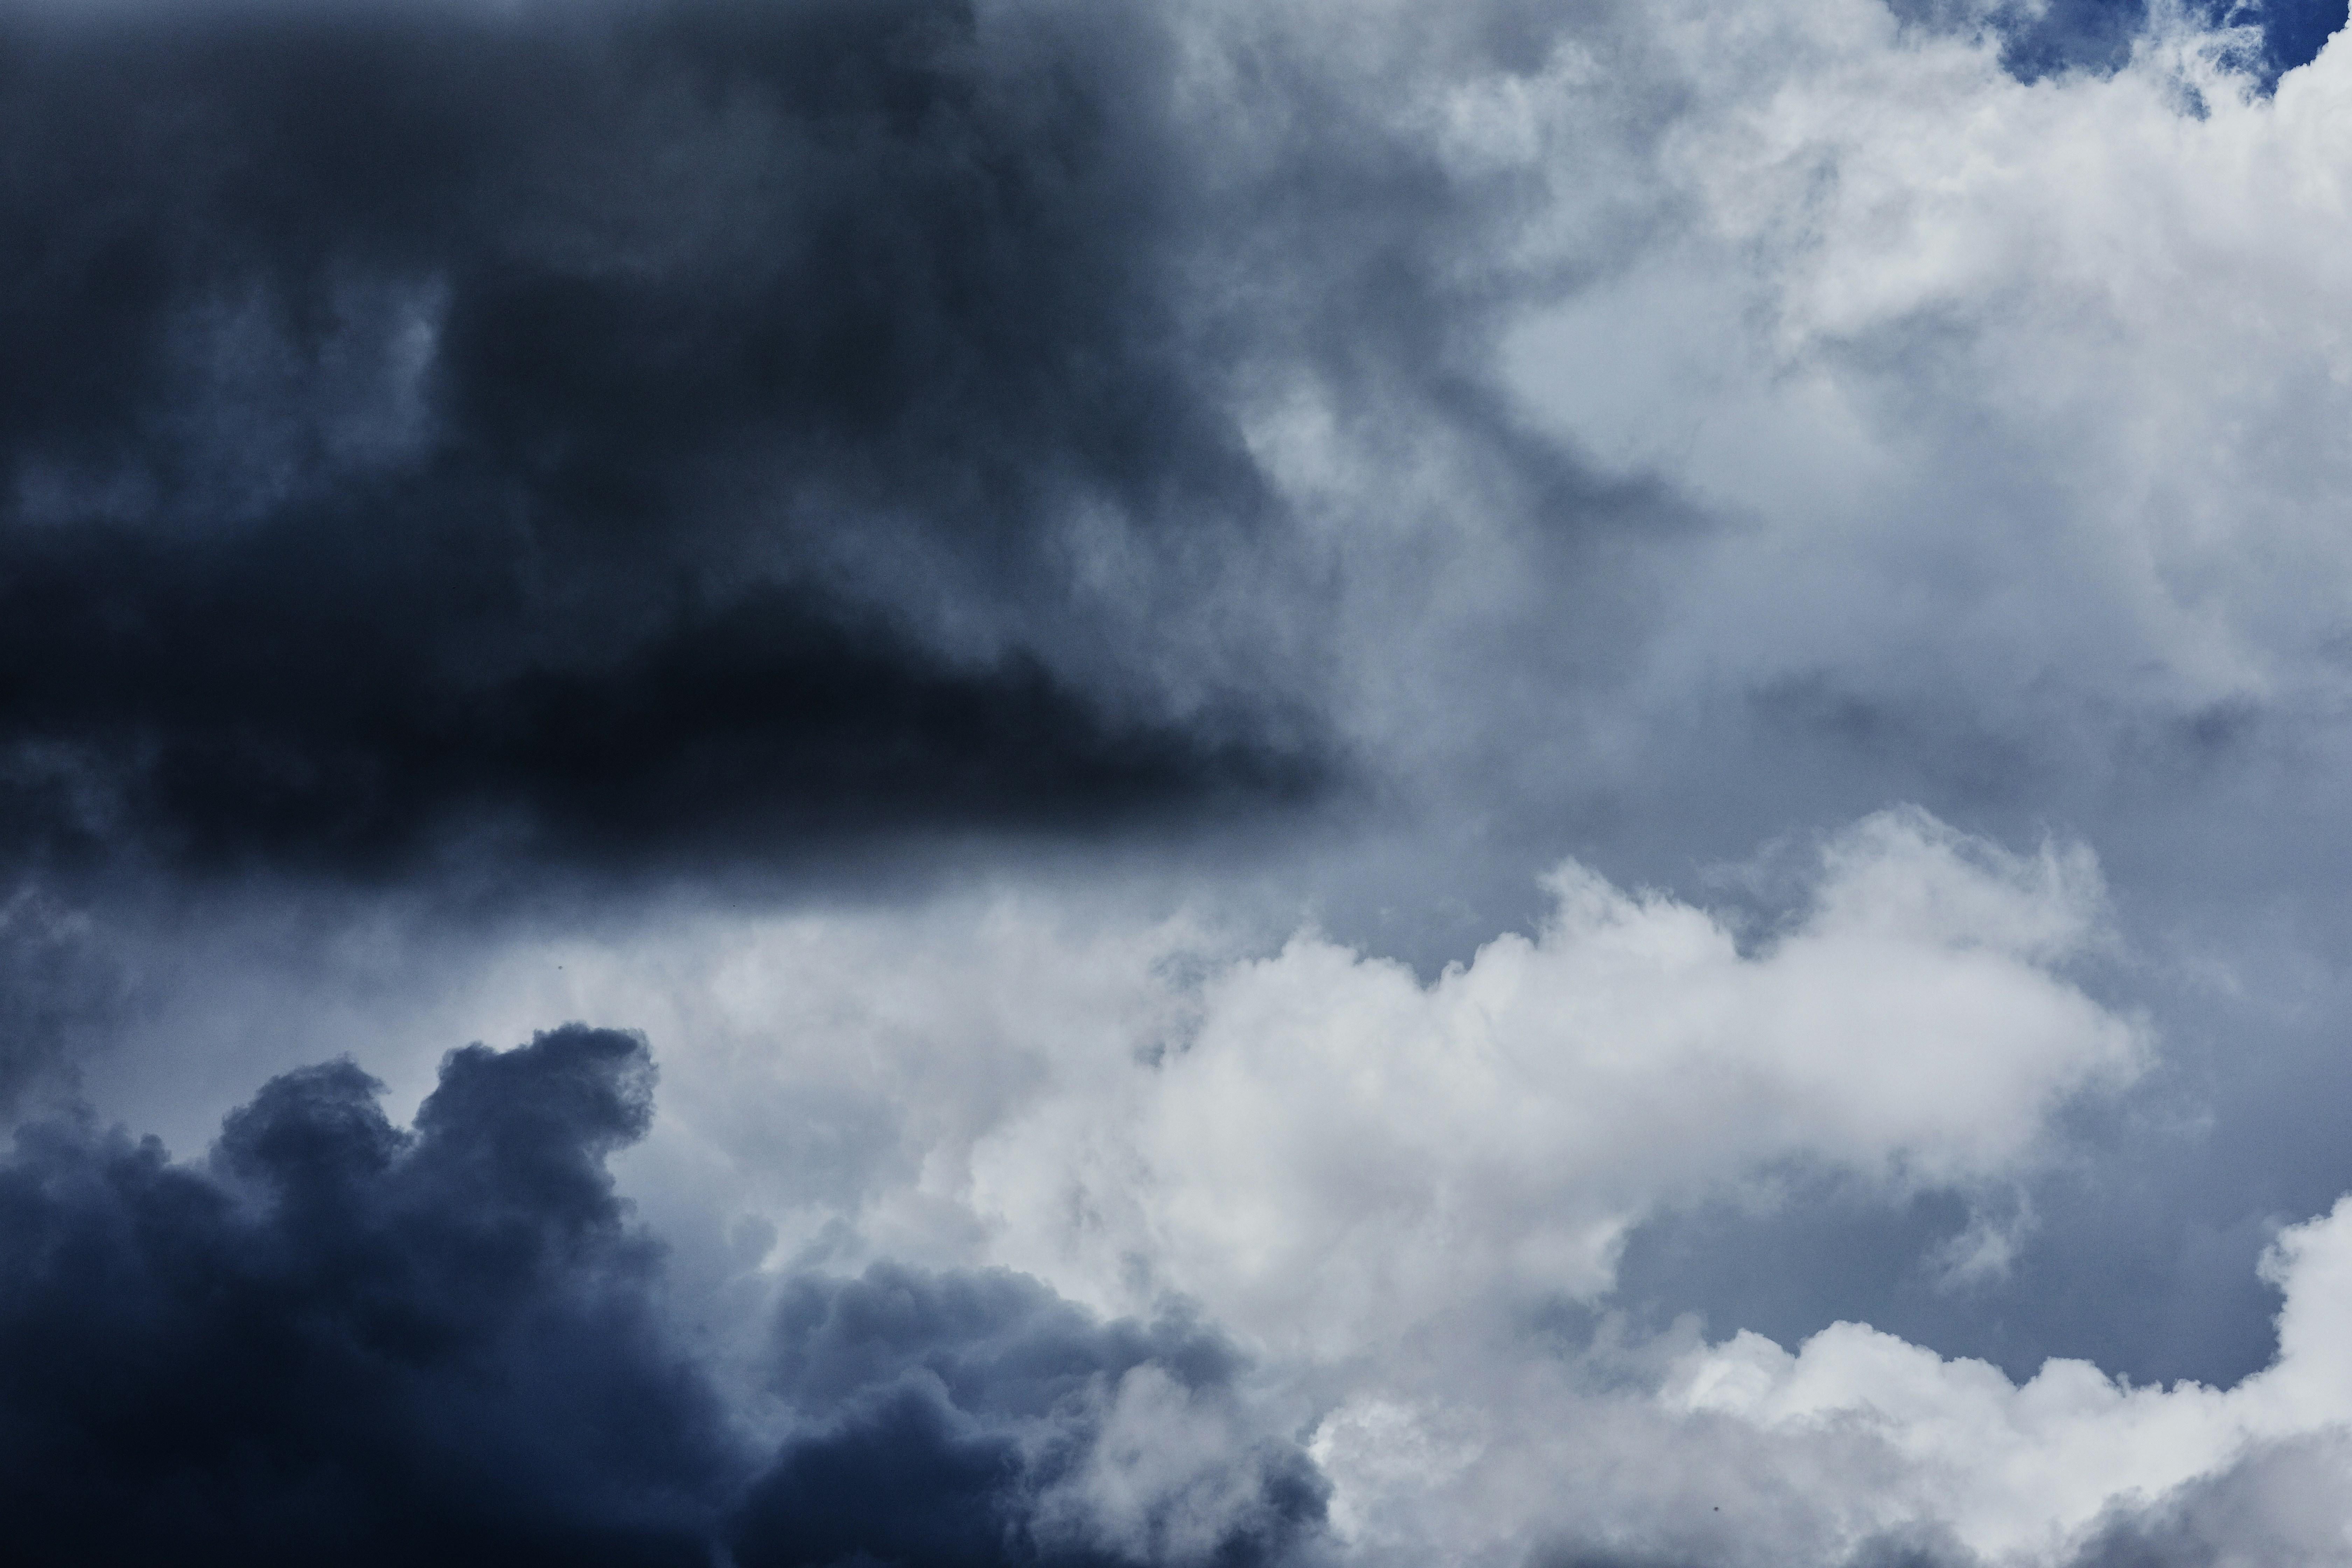
\includegraphics[width=\textwidth]{figures/black_clouds.jpg}
	\end{subfigure}
	\begin{subfigure}{0.45\textwidth}
		\center
		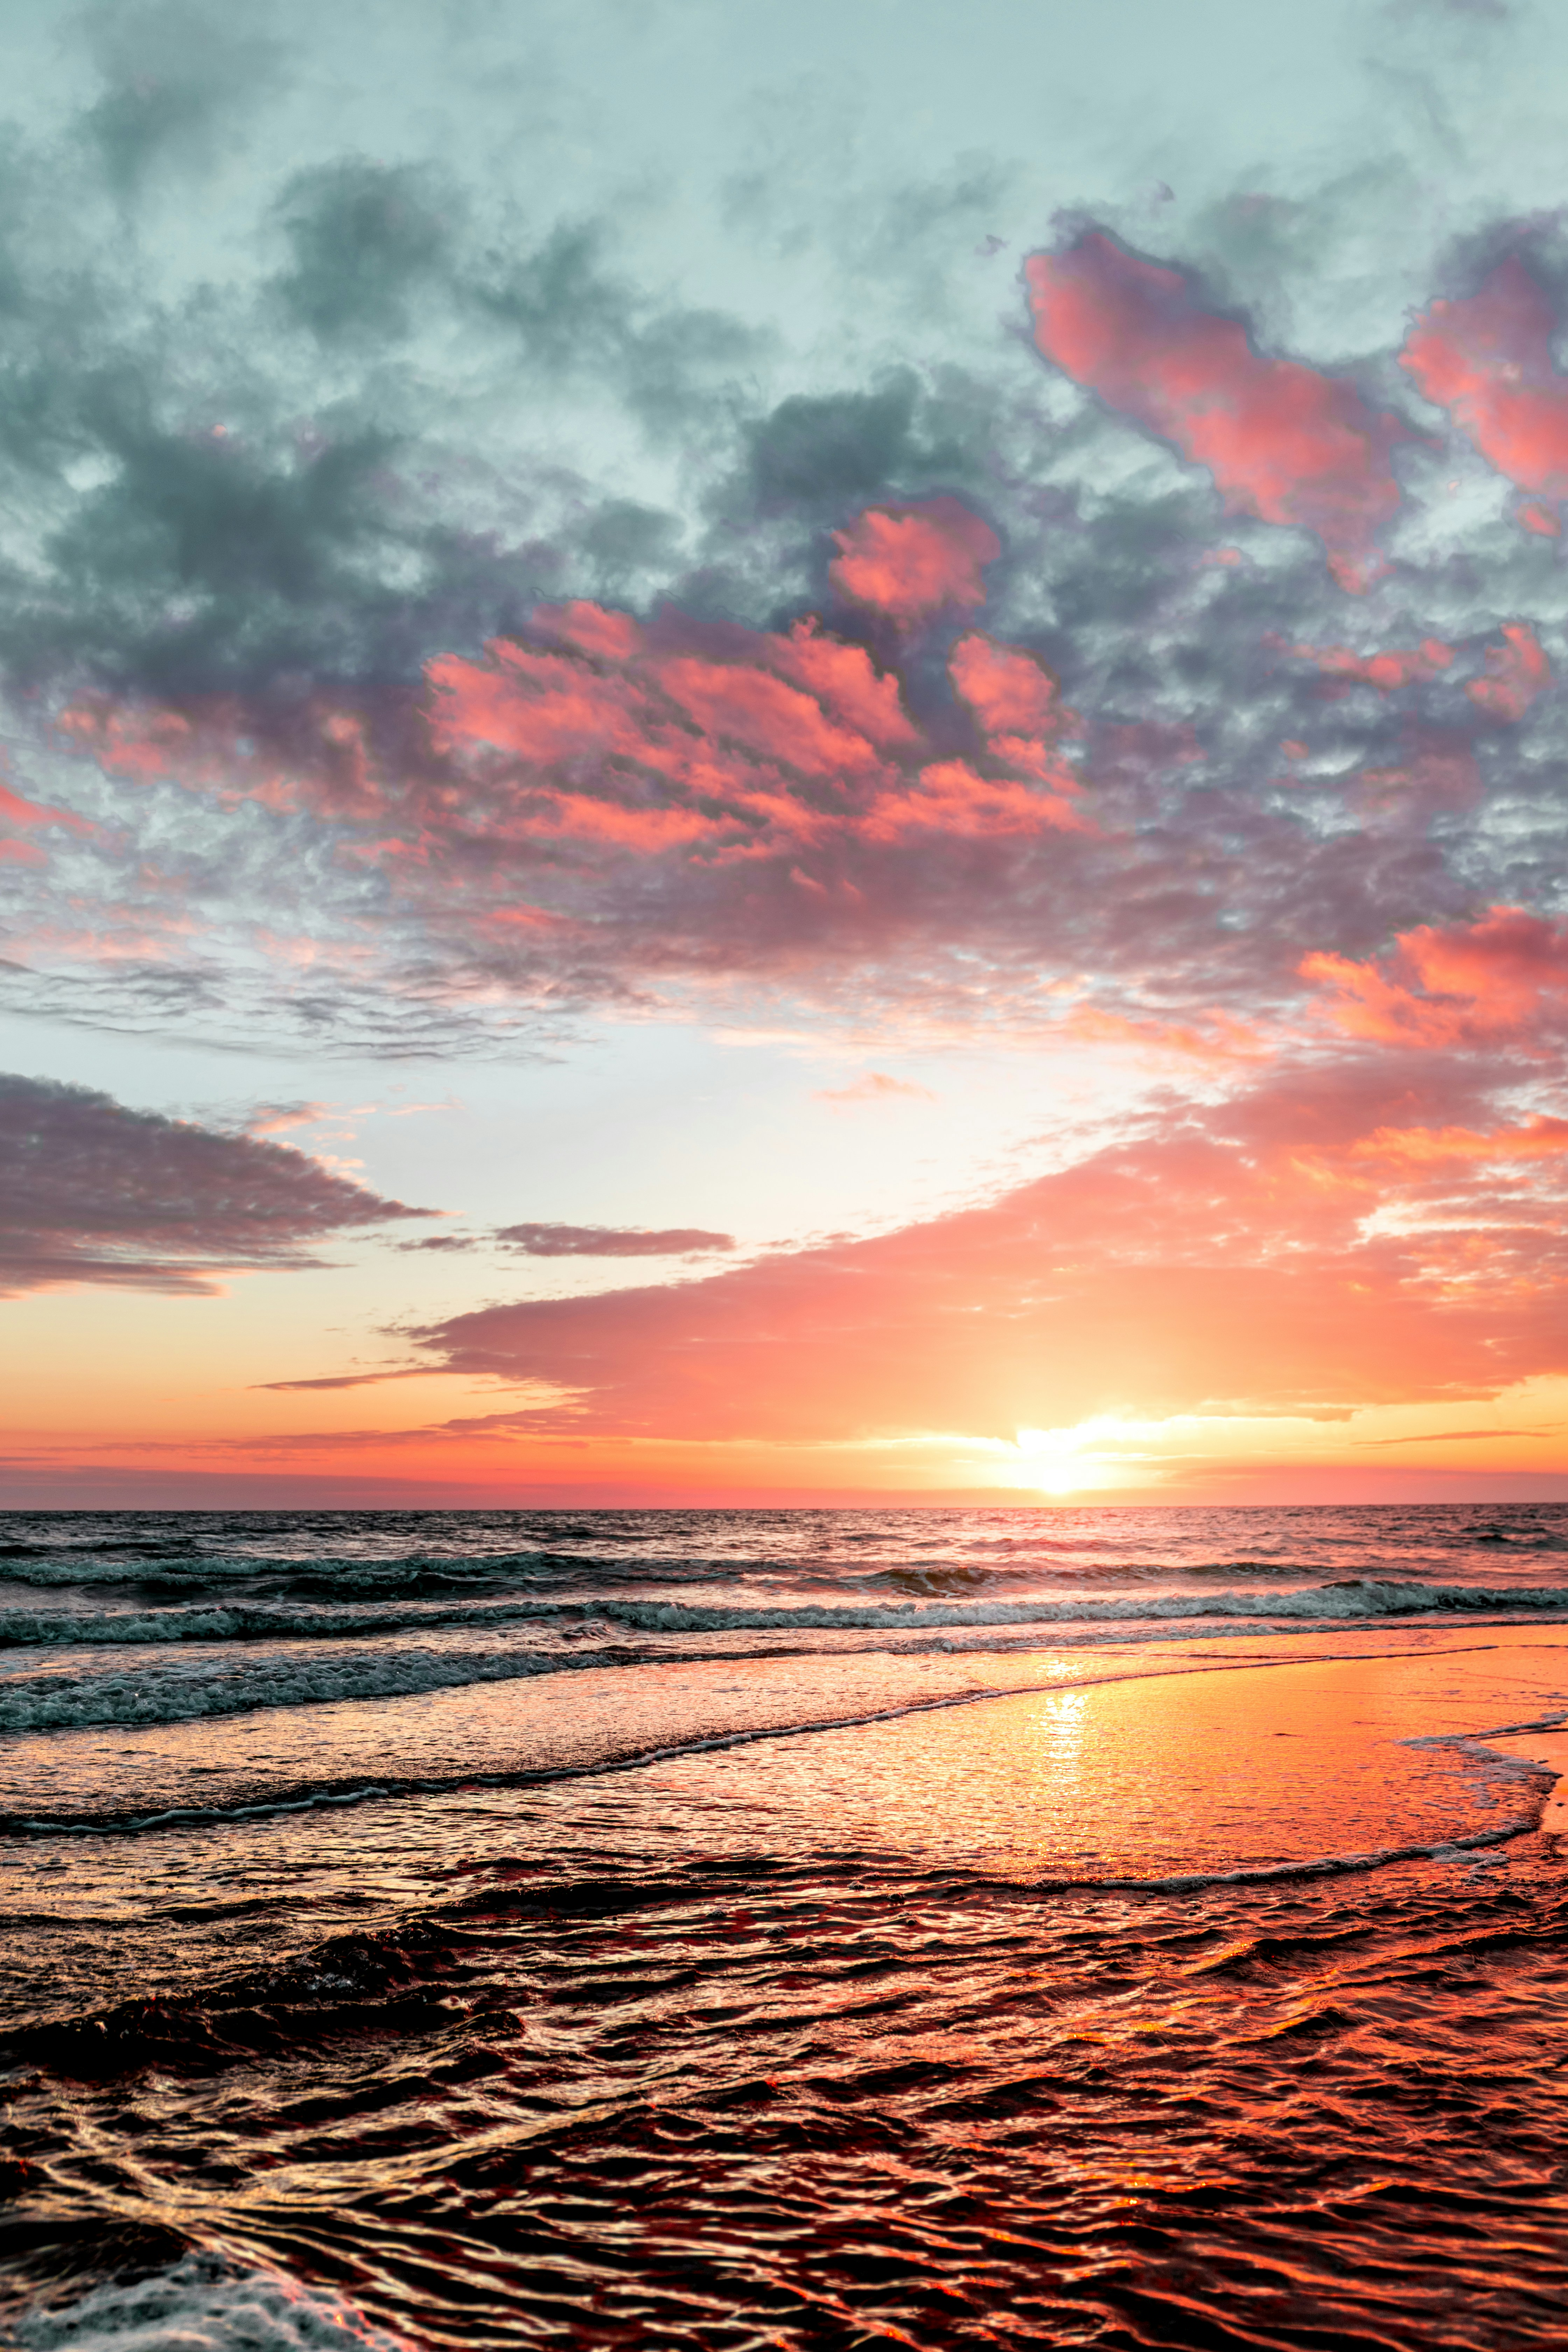
\includegraphics[width=0.5\textwidth]{figures/sunset.jpg}
	\end{subfigure}
\end{figure}

\footnotetext{\url{https://unsplash.com/fr/photos/nuages-blancs-et-ciel-bleu-a33De5Sn8xo}}

\footnotetext{\url{https://unsplash.com/fr/photos/plan-deau-sous-ciel-nuageux-au-coucher-du-soleil-HRX5WXFyB64}}

\end{frame}
%---------------------------------------------------------------------------
\begin{frame}{Atmosphere transmittance: absorption}


\begin{figure}
	\center
	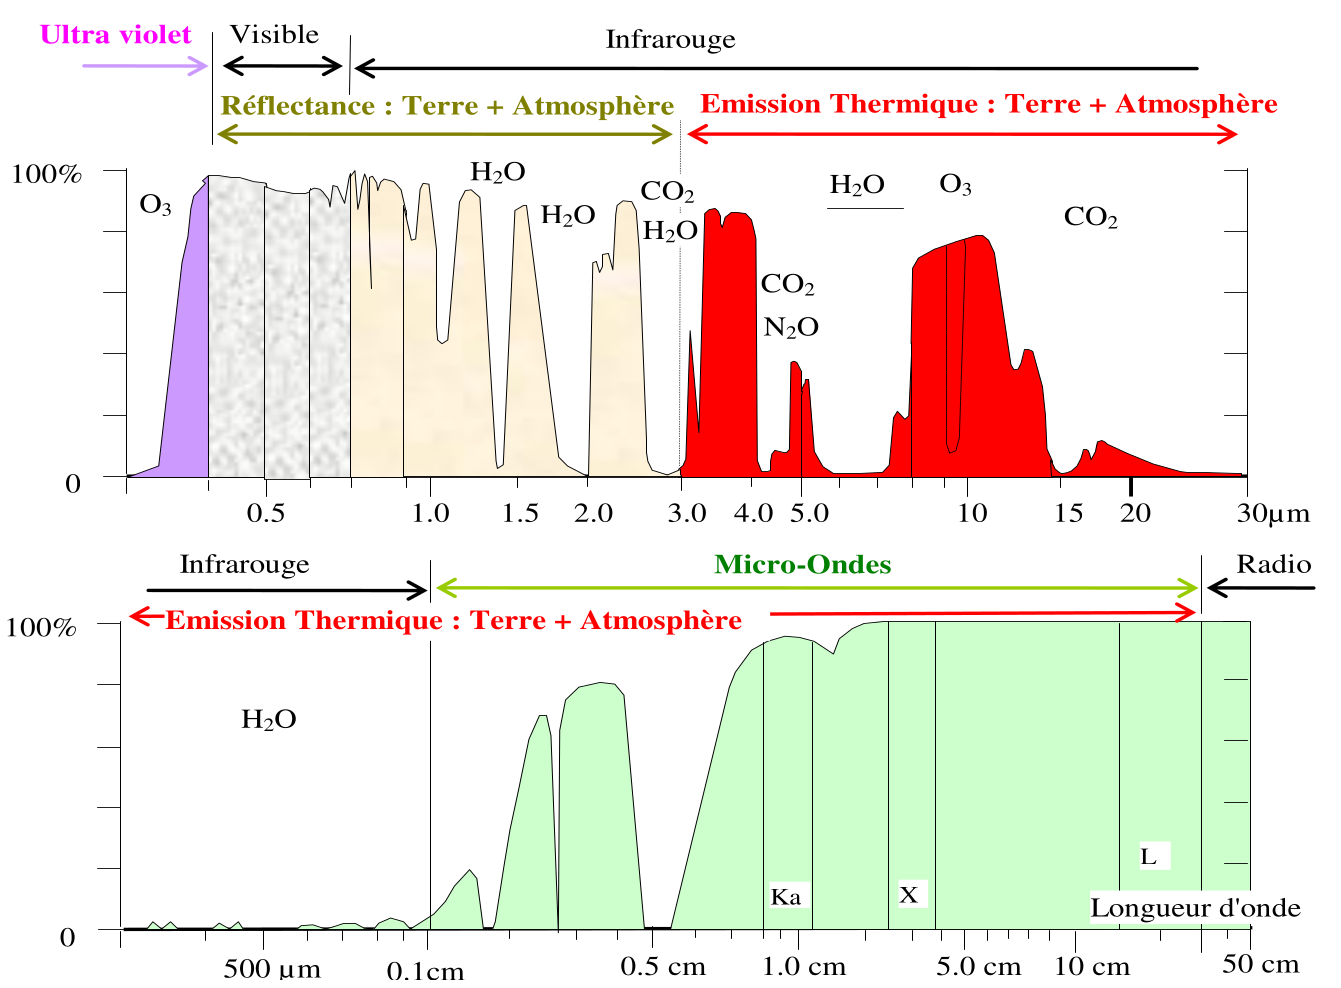
\includegraphics[width=0.65\textwidth]{figures/transmittance_atm.png}
	\caption{Atmospheric transmittance. Credit: J.P. Gastellu-Etchegorry}
\end{figure}

\end{frame}
%---------------------------------------------------------------------------
\begin{frame}{From top-of-atmosphere (TOA) to bottom-of-atmosphere (BOA) irradiance}

The total transmittance is the product of the transmittance due to scattering with all transmittances due to gas absorption.

\begin{columns}

\column{0.55\textwidth}

\begin{figure}
	\center
	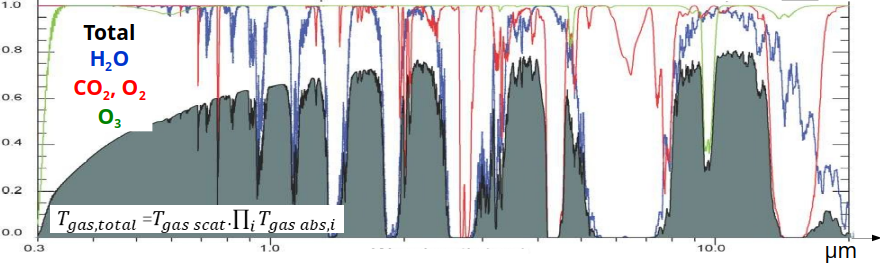
\includegraphics[width=\textwidth]{figures/tot_transmittance.png
}
	\caption{Illustration of total atmospheric transmittance (US STD76 gas model). Credit: J.P. Gastellu-Etchegorry}
\end{figure}

\column{0.3\textwidth}

\begin{figure}
	\center
	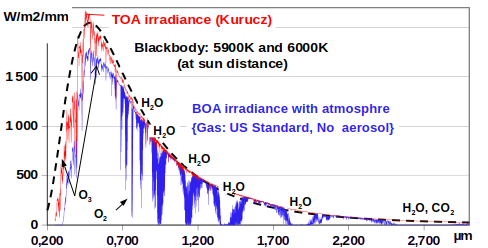
\includegraphics[width=\textwidth]{figures/toa_irradiance.png}
	\caption{Illustration of TOA and BOA sun irradiance. Credit: J.P. Gastellu-Etchegorry}
\end{figure}

\end{columns}

\end{frame}
%---------------------------------------------------------------------------
\begin{frame}{Reflectance}

%Given the top-of-atmosphere radiance $L(\lambda)$, the bottom-of-atmosphere solar irradiance $E(\lambda)$, and the sun zenith angle $\theta$, it is defined as:

Reflectance is the physical quantity of interest: it only depends on the \textbf{surface chemical composition and rugosity}. For a surface $\Sigma$ and a direction $\Omega$, reflectance is defined as follows:
\begin{align*}
	\rho_{\Sigma, \lambda}(\Omega) = \frac{\pi \: R_{\Sigma, \lambda}(\Omega)}{I_{\Sigma, \lambda}}
\end{align*}
where $R_{\Sigma, \lambda}$ and $I_{\Sigma, \lambda}$ denote the surface radiance and irradiance at wavelength $\lambda$, respectively.
We usually assume Lambertian surfaces for which reflectance does not depend on the reflected direction $\Omega$.

\begin{figure}
	\center
	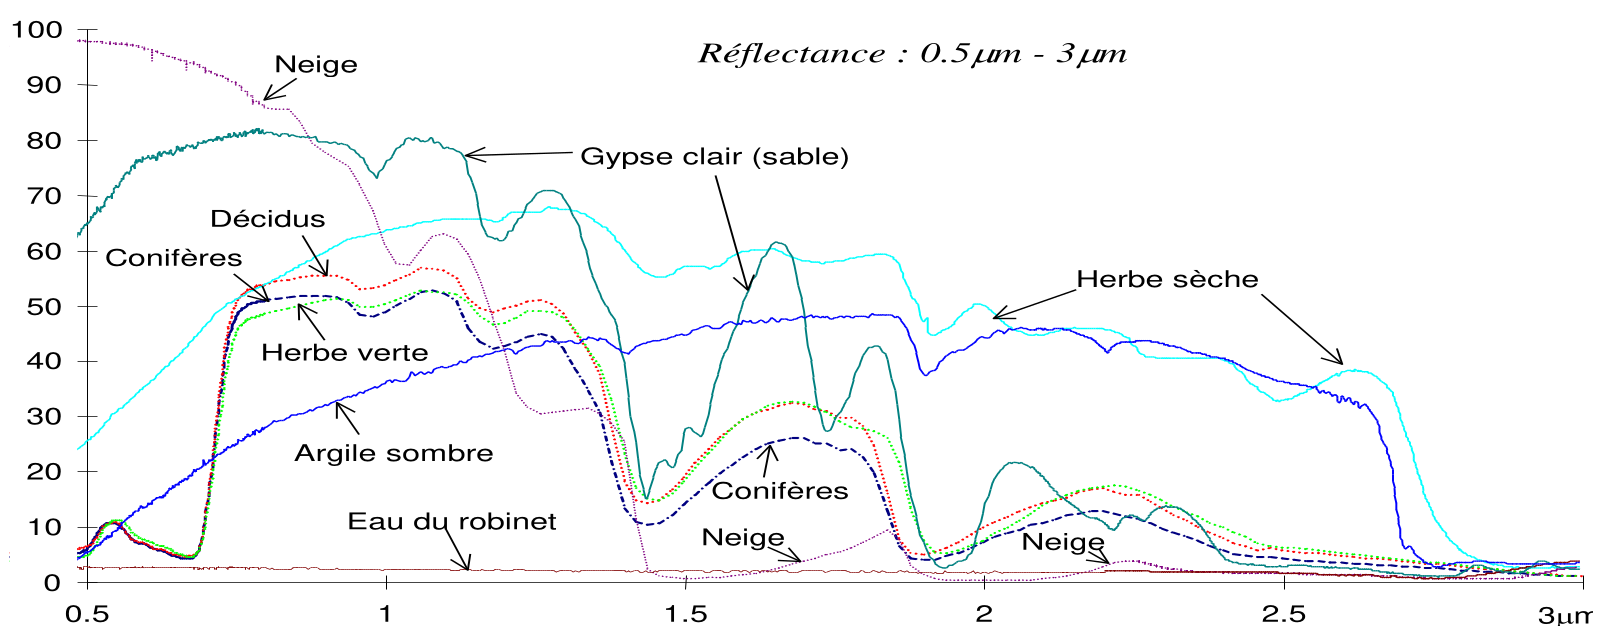
\includegraphics[width=0.6\textwidth]{figures/reflectance.png}
	\caption{Reflectance of several materials. Credit: J.P. Gastellu-Etchegorry}
\end{figure}

\end{frame}
%---------------------------------------------------------------------------
\begin{frame}{Bi-directional reflectance}

Natural surfaces may exhibit "hot-spot" effects or "specular" reflection.

\begin{figure}
	\center
	\begin{subfigure}{0.45\textwidth}
		\center
		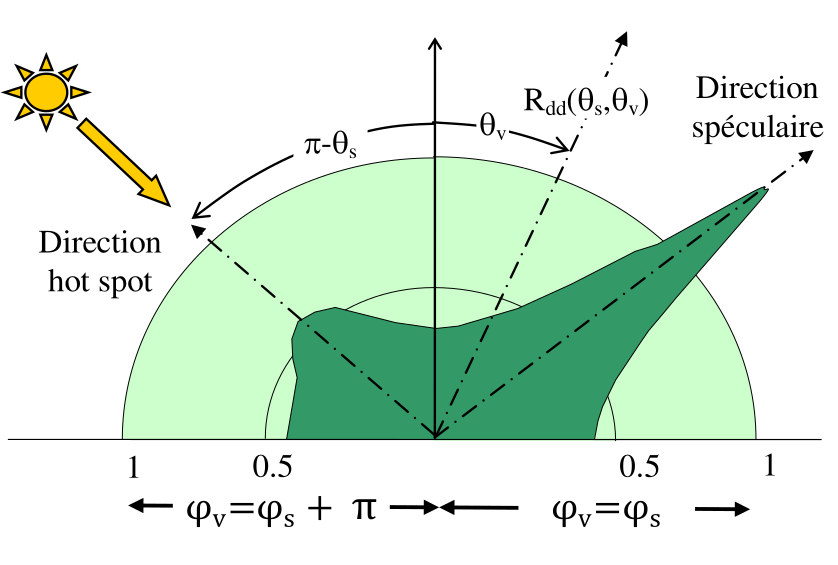
\includegraphics[width=\textwidth]{figures/brdf.png}
		\caption{Illustration of bi-directional reflectance for a \textcolor{lightgreen}{Lambertian surface} and a \textcolor{darkgreen}{natural surface} with specular reflection. Credit: J.P. Gastellu-Etchegorry}
	\end{subfigure}
	\hfill
	\begin{subfigure}{0.45\textwidth}
		\center
		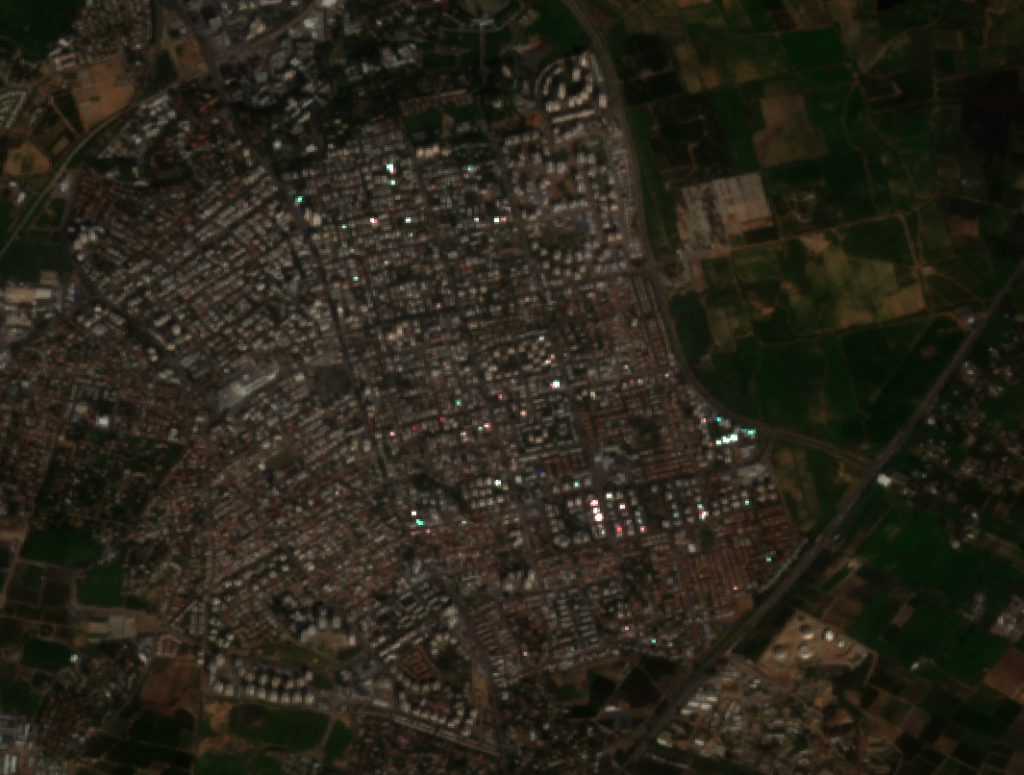
\includegraphics[width=\textwidth]{figures/Roof_Windows-1024x775.png}
		\caption{Reflectances greater than one observed over roof windows in a VENµS (CNES, IAI ELOp) image. Source: \url{https://www.cesbio.cnrs.fr/multitemp/16885-2/}}
	\end{subfigure}
\end{figure}

$\blacktriangleright$ \textit{Show that, for a Lambertian surface, reflectance is lower or equal to one.}

\end{frame}
%---------------------------------------------------------------------------
\begin{frame}{Reflectance time series}

As much as reflectance is intrinsic to the surface properties, it is the natural quantity to monitor the ecosystems through time, with changes in sun zenith angle, Earth-sun distance, and atmospheric variations...

\begin{figure}
	\center
	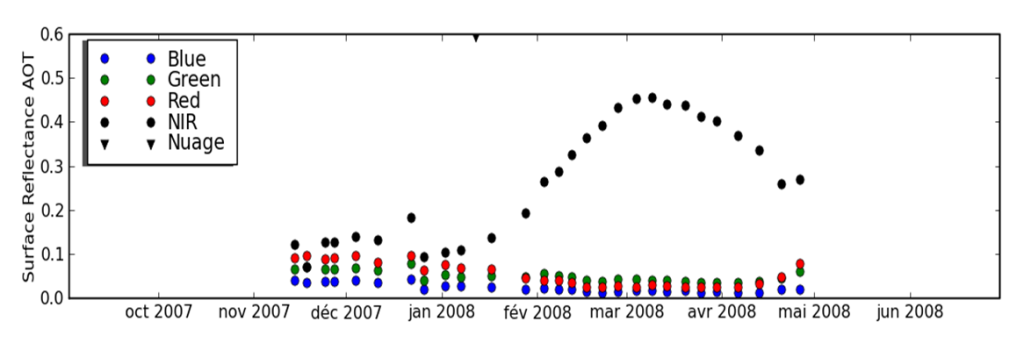
\includegraphics[width=0.6\textwidth]{figures/profil_mexique-1024x350.png}
	\caption{Reflectance of a wheat field as a function of time for 4 spectral bands from a time series of Formosat-2 images. Source: \url{https://www.cesbio.cnrs.fr/multitemp/radiometric-quantities-irradiance-radiance-reflectance/}}
\end{figure}

\end{frame}
%---------------------------------------------------------------------------
\begin{frame}{What does the sensor measure?}

Surface radiance $R_{\Sigma, \lambda}(\Omega) = \rho_{\Sigma, \lambda}(\Omega) \times I_{\Sigma, \lambda} / \pi$ is not what is measured by the sensor. 

\begin{figure}
	\center
	\begin{subfigure}{0.25\textwidth}
		\center
		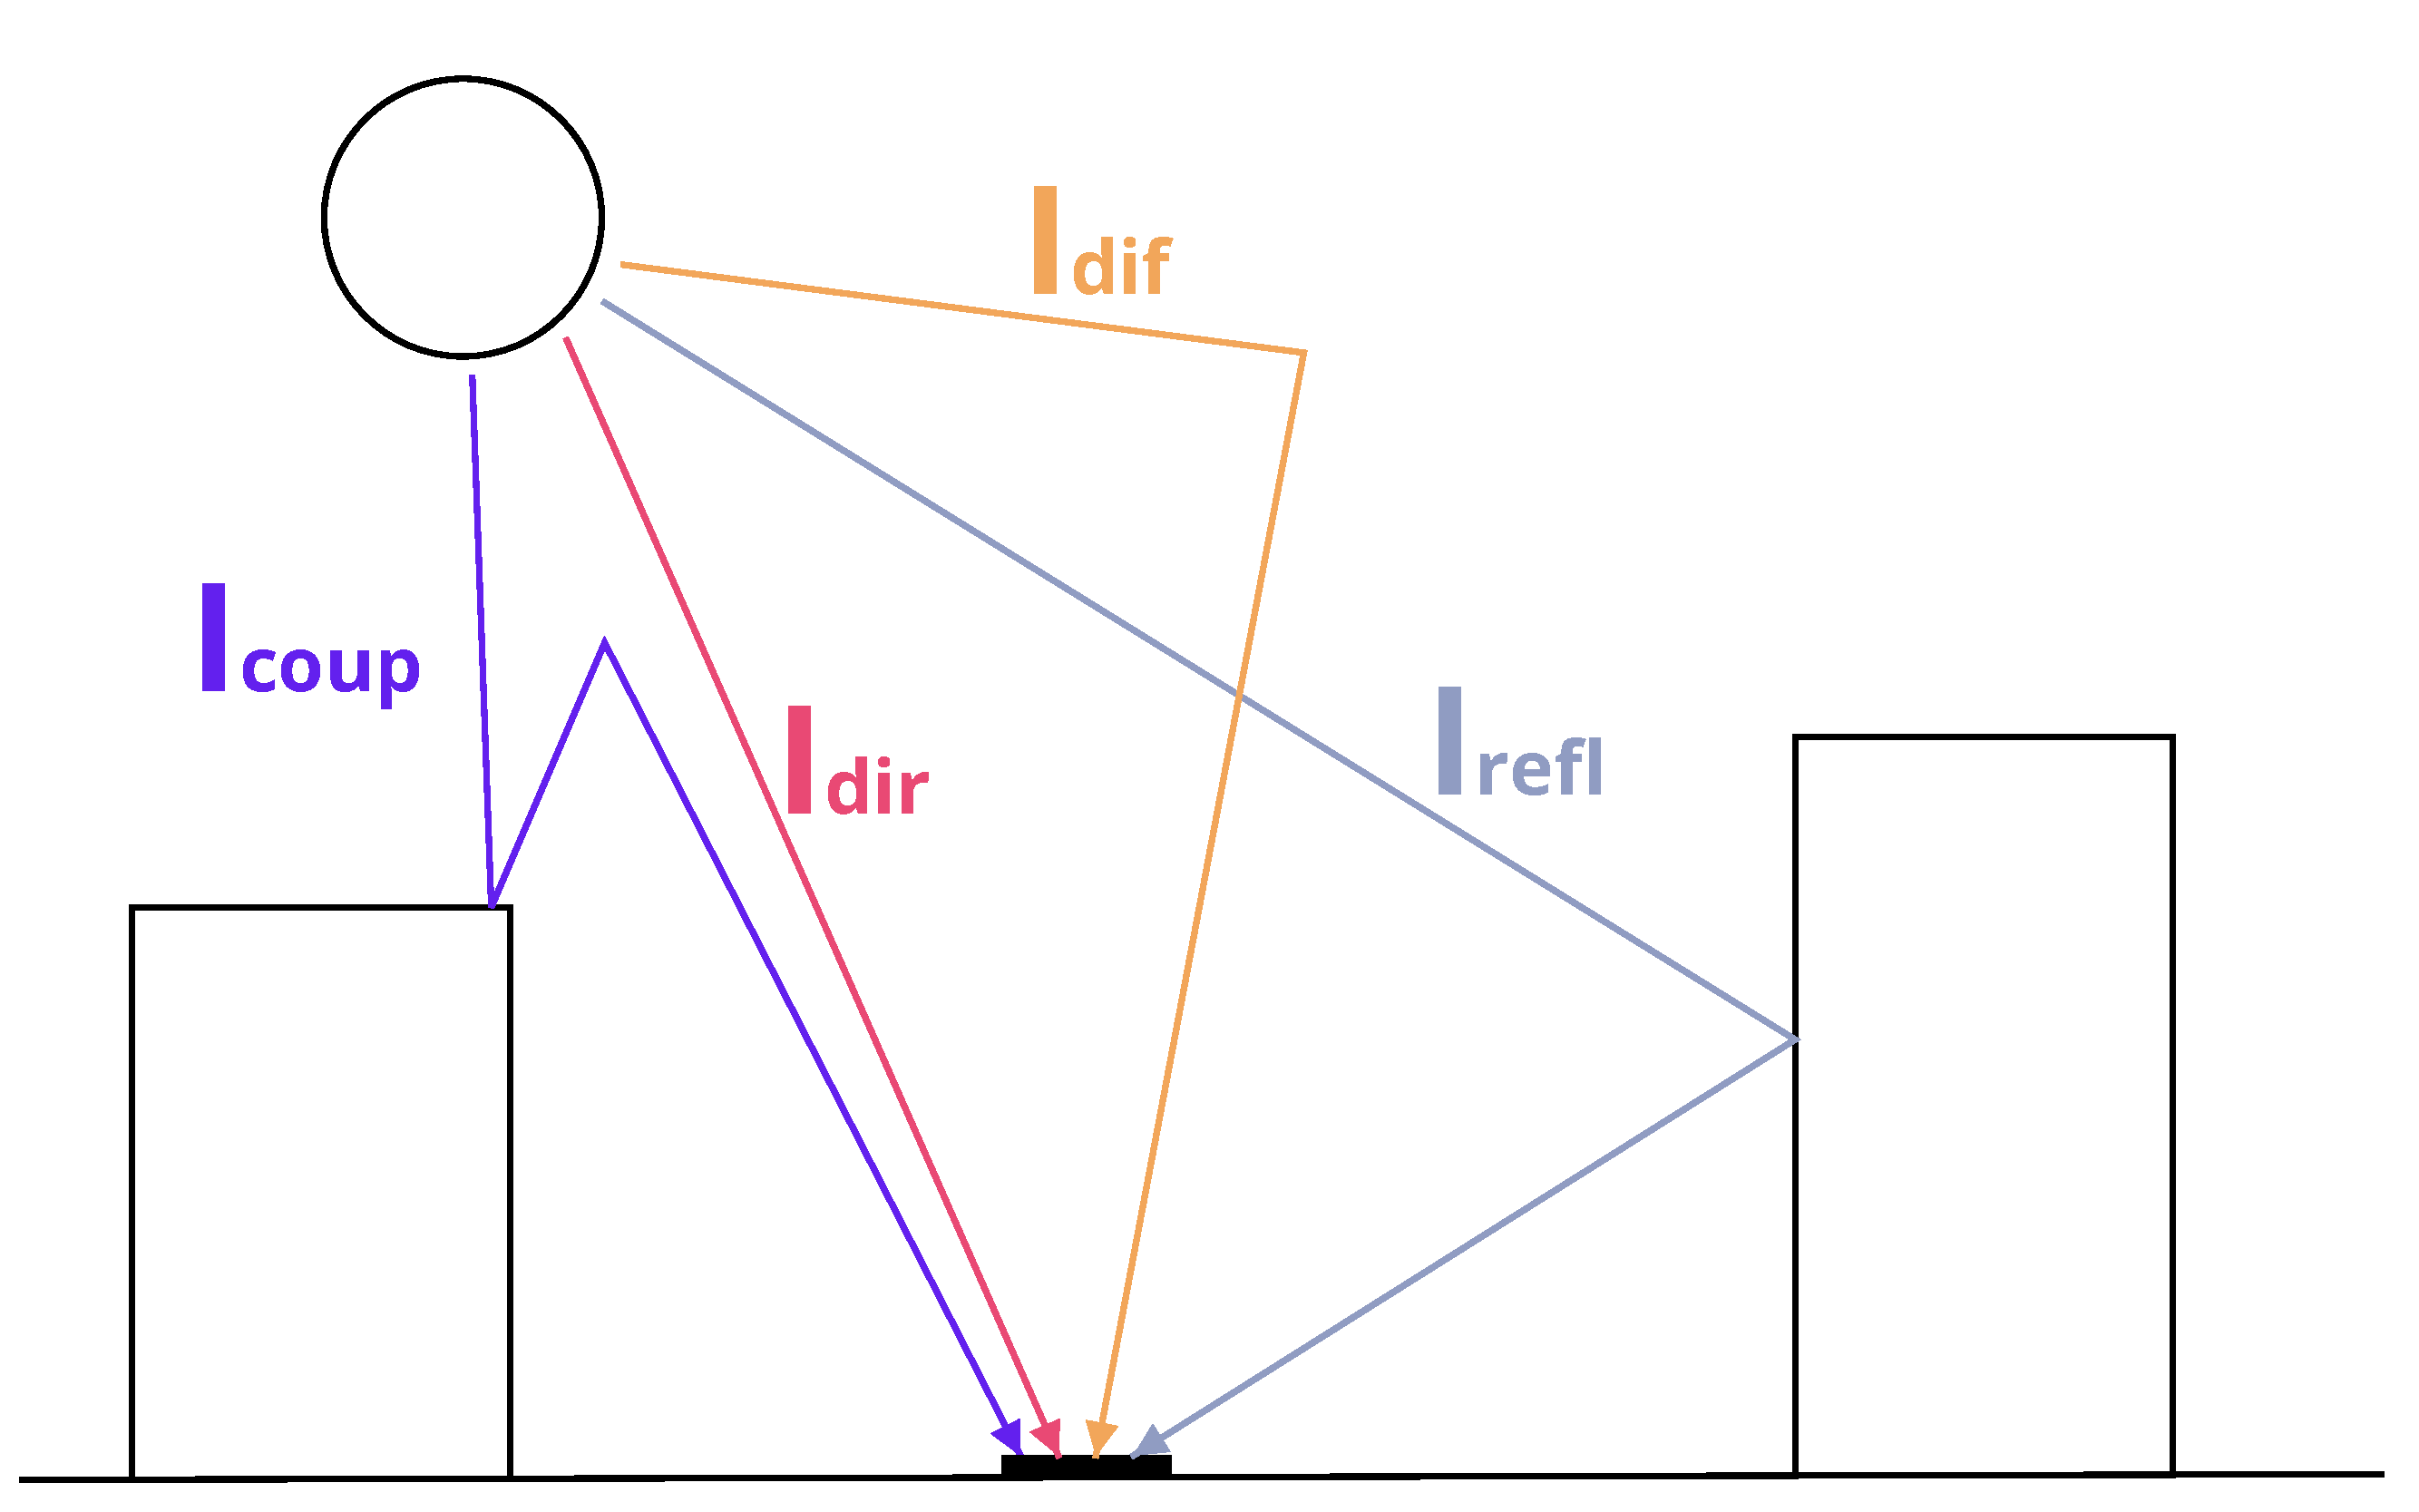
\includegraphics[width=\textwidth]{figures/I_terms.pdf}
		\caption{Irradiance terms}
	\end{subfigure}
	\hspace{0.1cm}
	\begin{subfigure}{0.25\textwidth}
		\center
		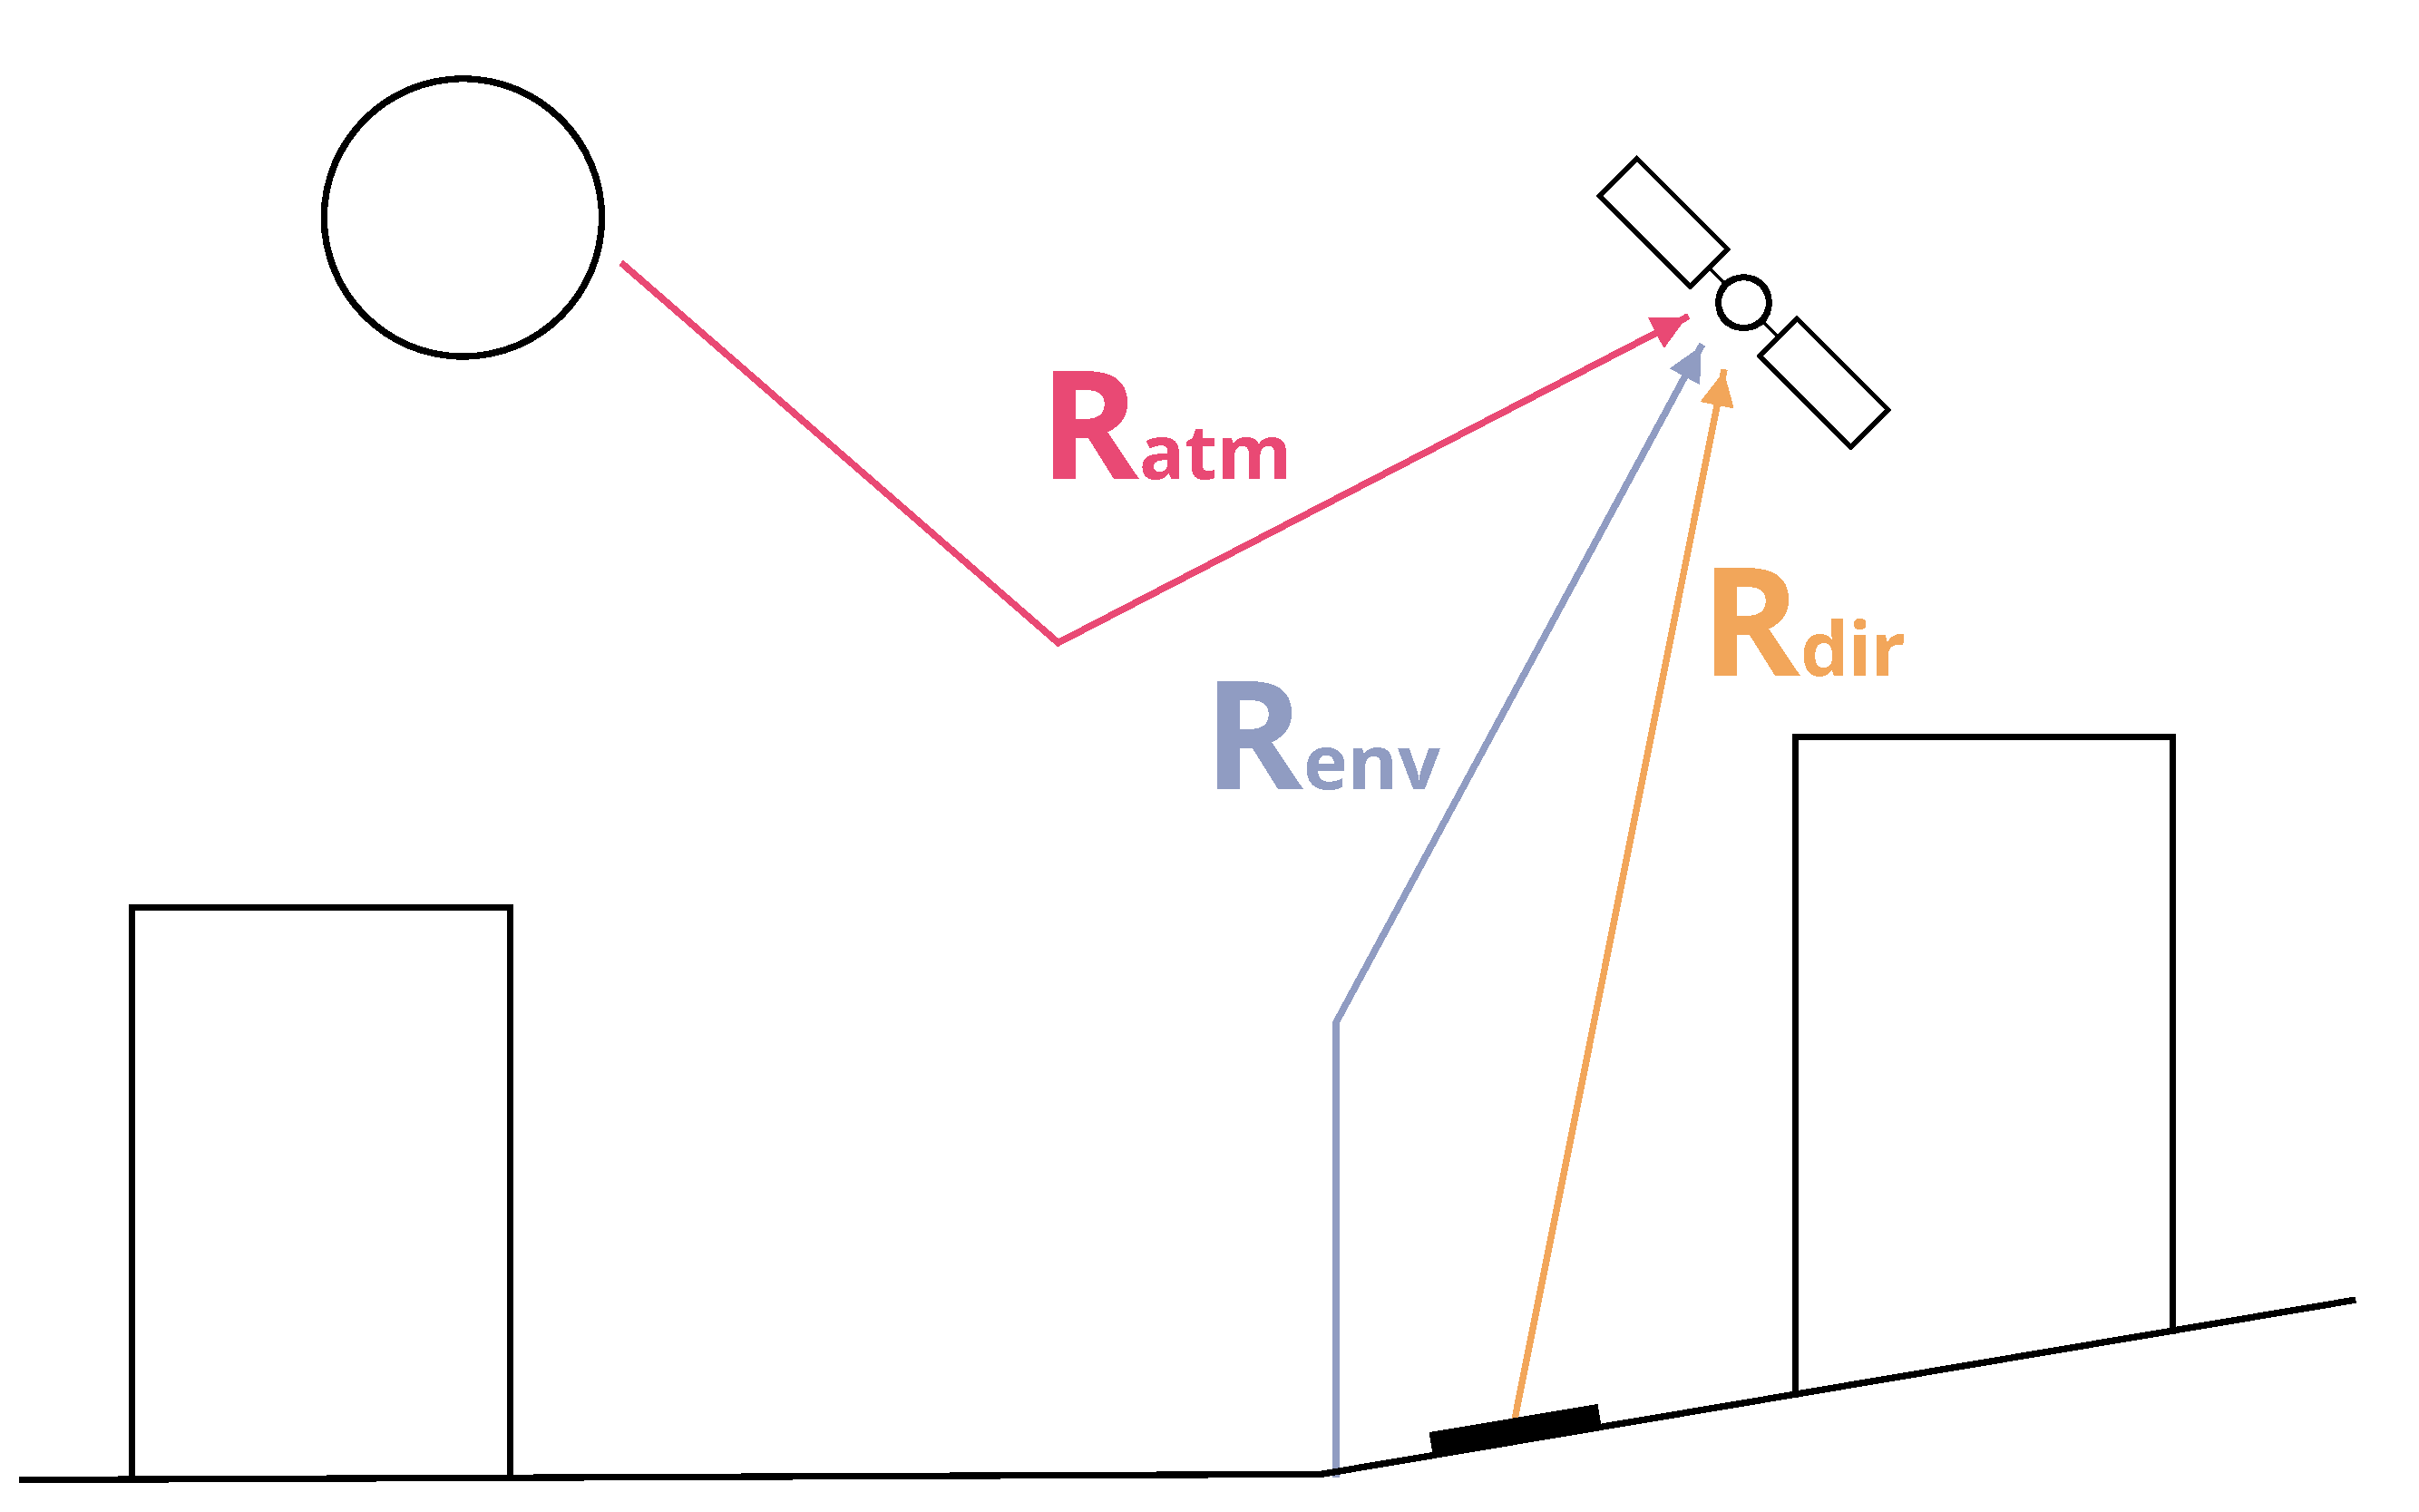
\includegraphics[width=\textwidth]{figures/R_terms.pdf}
		\caption{Radiance terms}
	\end{subfigure}
	\caption{Illustration of the contributions of atmosphere to the measured signal}
\end{figure}

We have that:
\begin{align*}
	I_{\Sigma, \lambda} & = \overbrace{I_{\text{dir}, \lambda}}^{I_{\text{sun}, \text{BOA}, \lambda} \: \text{cos } \theta_{\text{sun}, \Sigma}} + I_{\text{dif}, \lambda} + I_{\text{refl}, \lambda} + I_{\text{coupl}, \lambda} \\
	R_{\text{sensor}, \lambda} & =  R_{\text{atm}, \lambda} + \underbrace{R_{\text{dir}, \lambda}}_{R_{\Sigma, \lambda} \times \tau_{\text{dir}, \lambda}} + R_{\text{env}, \lambda}
\end{align*}
where $\text{cos } \theta_{\text{sun}, \Sigma}$ is the sun zenith angle, and $\tau_{\text{dir}, \lambda}$ is the direct upward transmittance. 
\end{frame}
%---------------------------------------------------------------------------
\begin{frame}{Atmospheric correction}

Atmospheric correction codes aim to estimate the \textbf{surface-level reflectance} from the \textbf{sensor-level radiance} and the atmosphere parameters. Let us denote $I_0 = I_{\text{dir}} + I_{\text{dif}}$ the irradiance term without interactions with the Earth. Neglecting the term $I_{\text{refl}}$, the total irradiance can be modeled as:
\begin{align*}
	I_{\Sigma} = I_0 + I_0 \: \rho_{\text{env}} \: S + I_0 \: (\rho_{\text{env}} \: S)^2 + \ldots = \frac{I_0}{1 - \rho_{\text{env}} \: S} \quad (\text{for } \rho_{\text{env}} S < 1) 
\end{align*}
where $\rho_{\text{env}}$ and $S$ are the environment reflectance and the atmospheric backscattering coefficient also called spherical albedo (fraction of upward flux that is scattered back towards Earth). Therefore, we have that
\begin{align*}
	R_{\text{sensor}} = R_{\text{atm}} + \underbrace{\tau_{\text{dir}} \frac{I_0}{\pi (1 - \rho_{\text{env}} S)} \rho_{\Sigma}}_{=R_{\text{dir}}} + \underbrace{\tau_{\text{dif}} \frac{I_0}{\pi (1 - \rho_{\text{env}} S)} \rho_{\text{env}}}_{=R_{\text{env}}}
\end{align*}


$\blacktriangleright$ \textit{Assuming that $\rho_{\text{env}} = \rho_{\Sigma}$, write $\rho_{\Sigma}$ as a function of the radiative terms.} \vspace{0.2cm}

This is usually the first step of operational atmospheric correction codes such as COCHISE\footnote{Poutier, L., Miesch, C., Lenot, X., Achard, V., \& Boucher, Y. (2002, March). COMANCHE and COCHISE: two reciprocal atmospheric codes for hyperspectral remote sensing. In 2002 AVIRIS Earth Science and Applications Workshop Proceedings (pp. 1059-0889). Pasadena, CA, USA: Jet Propulsion Laboratory. \url{https://popo.jpl.nasa.gov/pub/docs/workshops/02_docs/2002_Poutier.pdf}}.

%\begin{align*}
%	\rho_{\text{TOA}} = \frac{\pi R_{\text{sensor}}}{I_{\text{sun}, \text{TOA}} \text{cos } \theta_{\text{sun}}}
%\end{align*}

\end{frame}
%%--------------------------------------------------------------------------
\begin{frame}{Atmospheric correction: from top-of-atmosphere to bottom-of-atmosphere reflectance}

Atmospheric correction codes, \textit{e.g.} MAJA (CNES / CESBIO), correct the measured signal from the effects of atmosphere. 

\begin{figure}
	\center
	\begin{subfigure}{0.45\textwidth}
		\center
		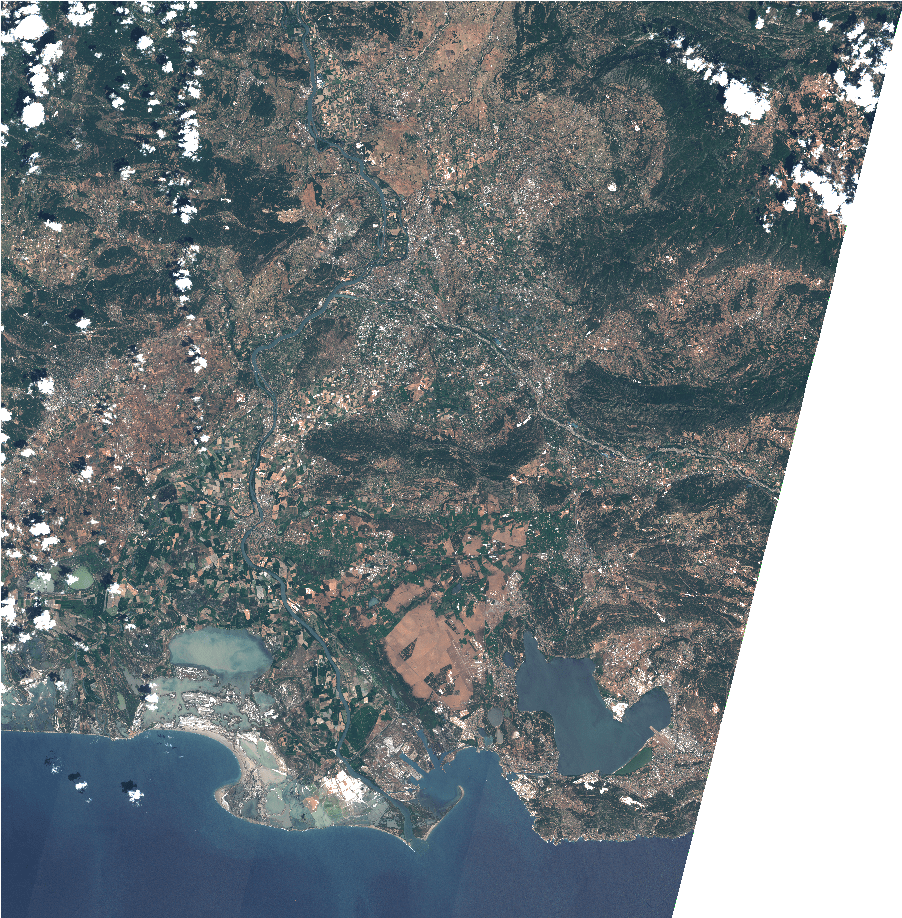
\includegraphics[width=0.6\textwidth]{figures/L1C.png}
		\caption{L1C level: Top-of-Atmosphere (TOA) reflectance data}
	\end{subfigure}
	\begin{subfigure}{0.45\textwidth}
		\center
		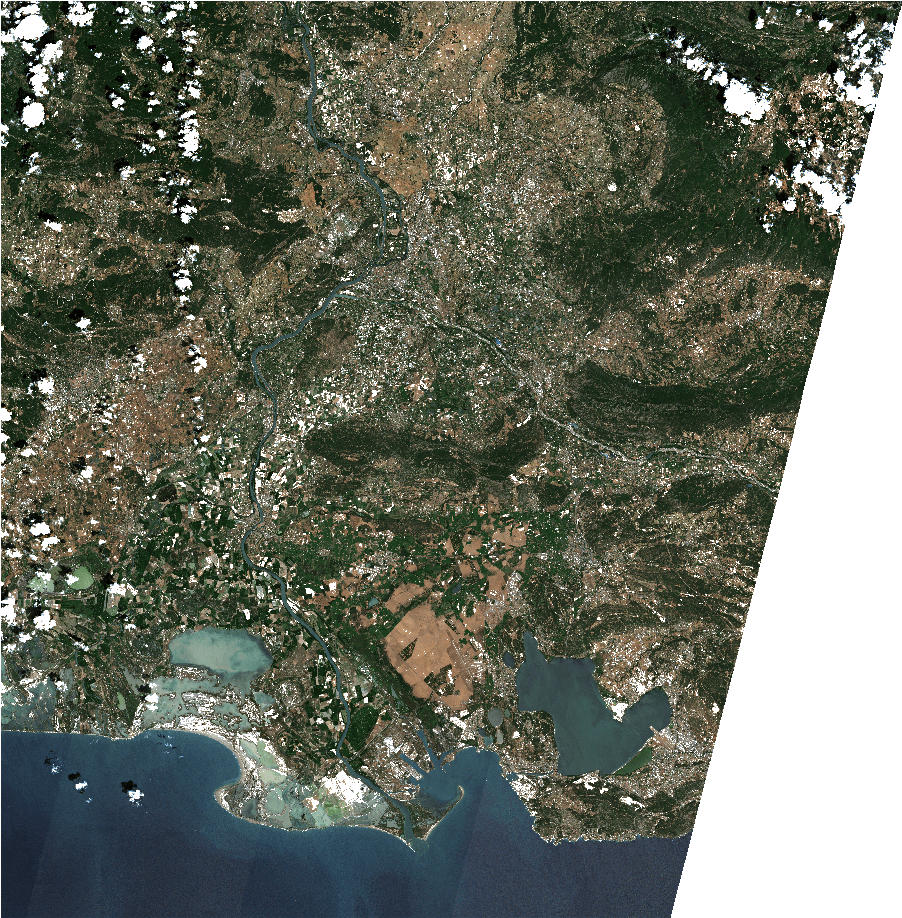
\includegraphics[width=0.6\textwidth]{figures/L2A.png}
		\caption{L2A level: Bottom-of-Atmosphere (BOA) reflectance data}
	\end{subfigure}
	\caption{Sentinel-2 images over Provence-Alpes-Côte-d'Azur. Credit: Copernicus, ESA, CNES.}
\end{figure}
\end{frame}
%---------------------------------------------------------------------------
\begin{frame}{Limitations of atmospheric correction}

\begin{figure}
	\center
	\begin{subfigure}{0.45\textwidth}
		\center
		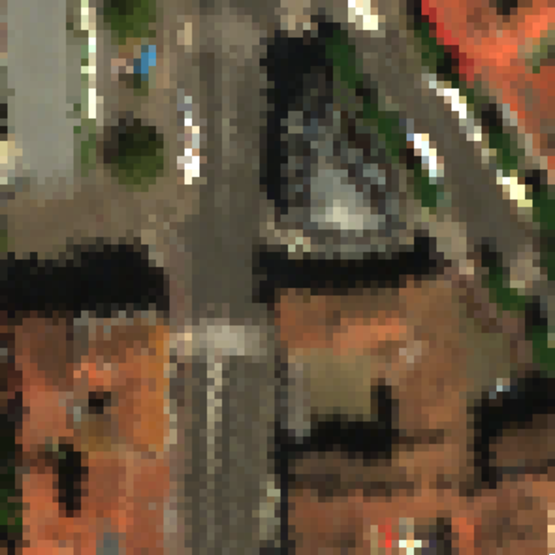
\includegraphics[width=0.6\textwidth]{figures/asphalt_hyp.pdf}
	\end{subfigure}
	\begin{subfigure}{0.45\textwidth}
		\center
		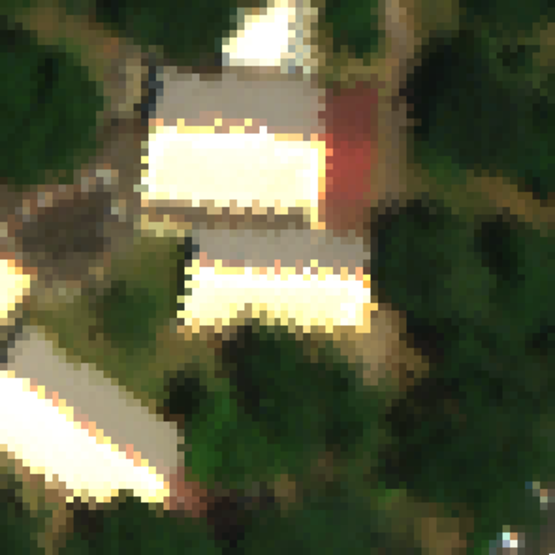
\includegraphics[width=0.6\textwidth]{figures/fib_hyp.pdf}
	\end{subfigure}
	\caption{RGB composition of a hyperspectral image with a 1m spatial resolution over Toulouse, France. Credit: ONERA-DOTA, Toulouse}
\end{figure}

\end{frame}
%---------------------------------------------------------------------------
%--------------------------------------------------------------------------
\subsection{Sentinel-2 multispectral sensor}
%---------------------------------------------------------------------------
\begin{frame}{Outline}
\tableofcontents[currentsection, currentsubsection]
\end{frame}
%--------------------------------------------------------------------------
\begin{frame}{Earth observation from space: the Copernicus program}

\begin{figure}
	\center
	\begin{subfigure}{0.45\textwidth}
		\center
		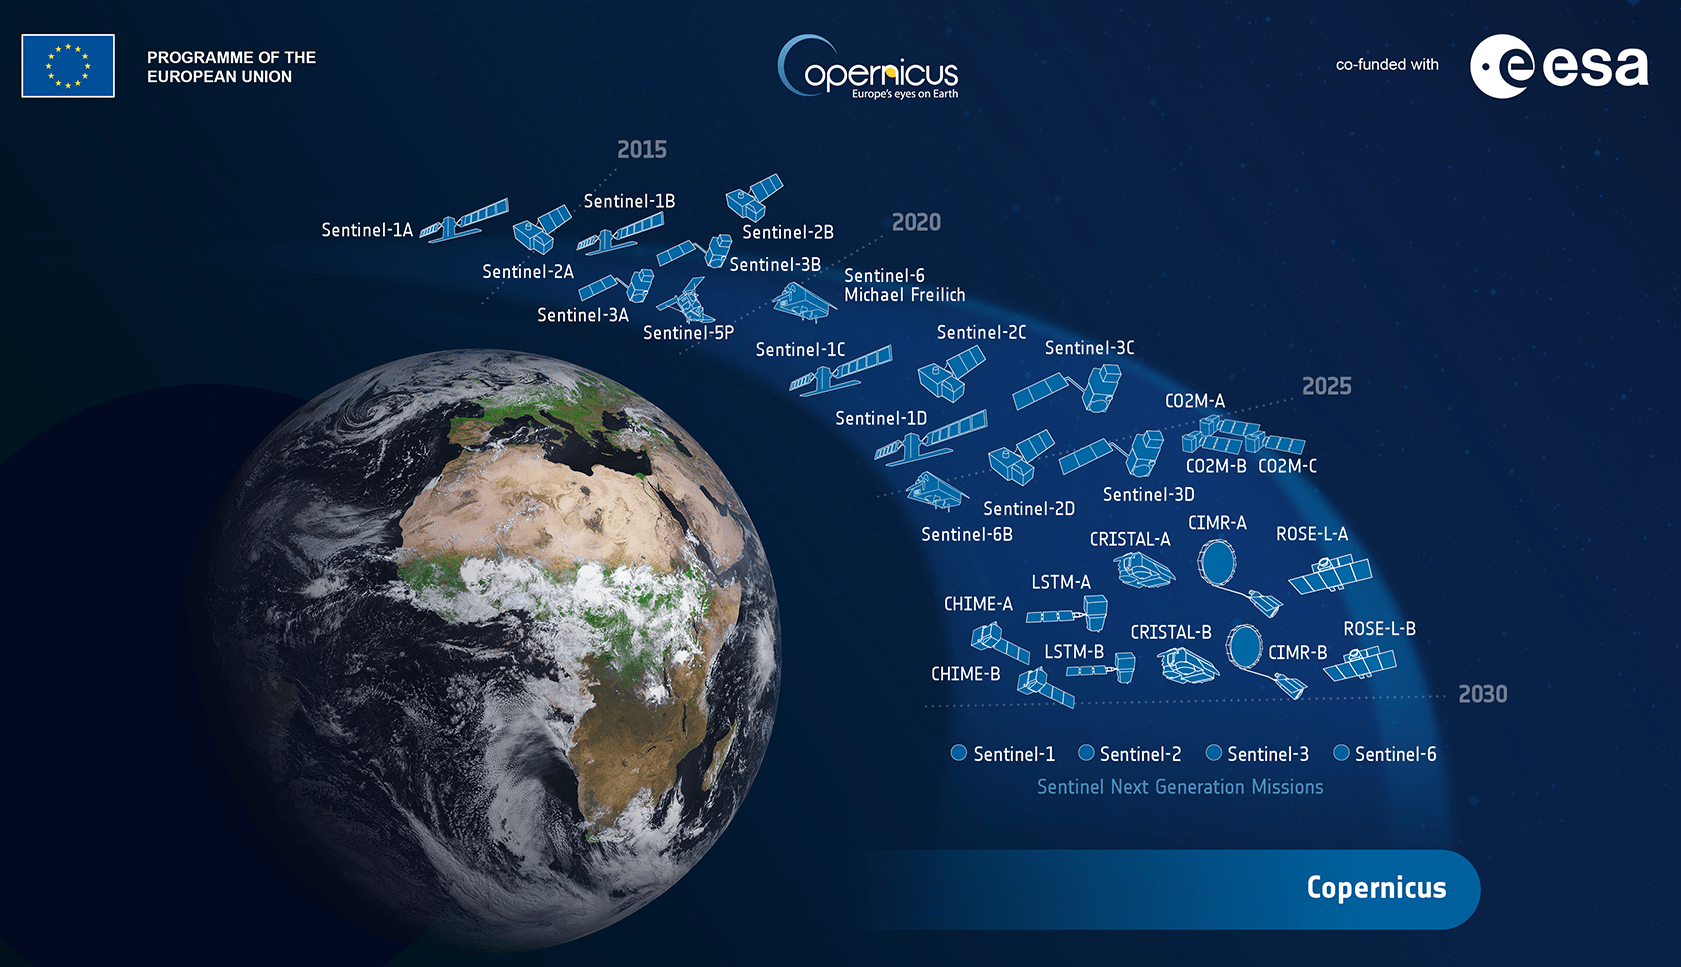
\includegraphics[width=\textwidth]{figures/copernicus.png}
		\caption{\url{https://www.copernicus.eu/fr}}
	\end{subfigure}
	\begin{subfigure}{0.45\textwidth}
		\center
		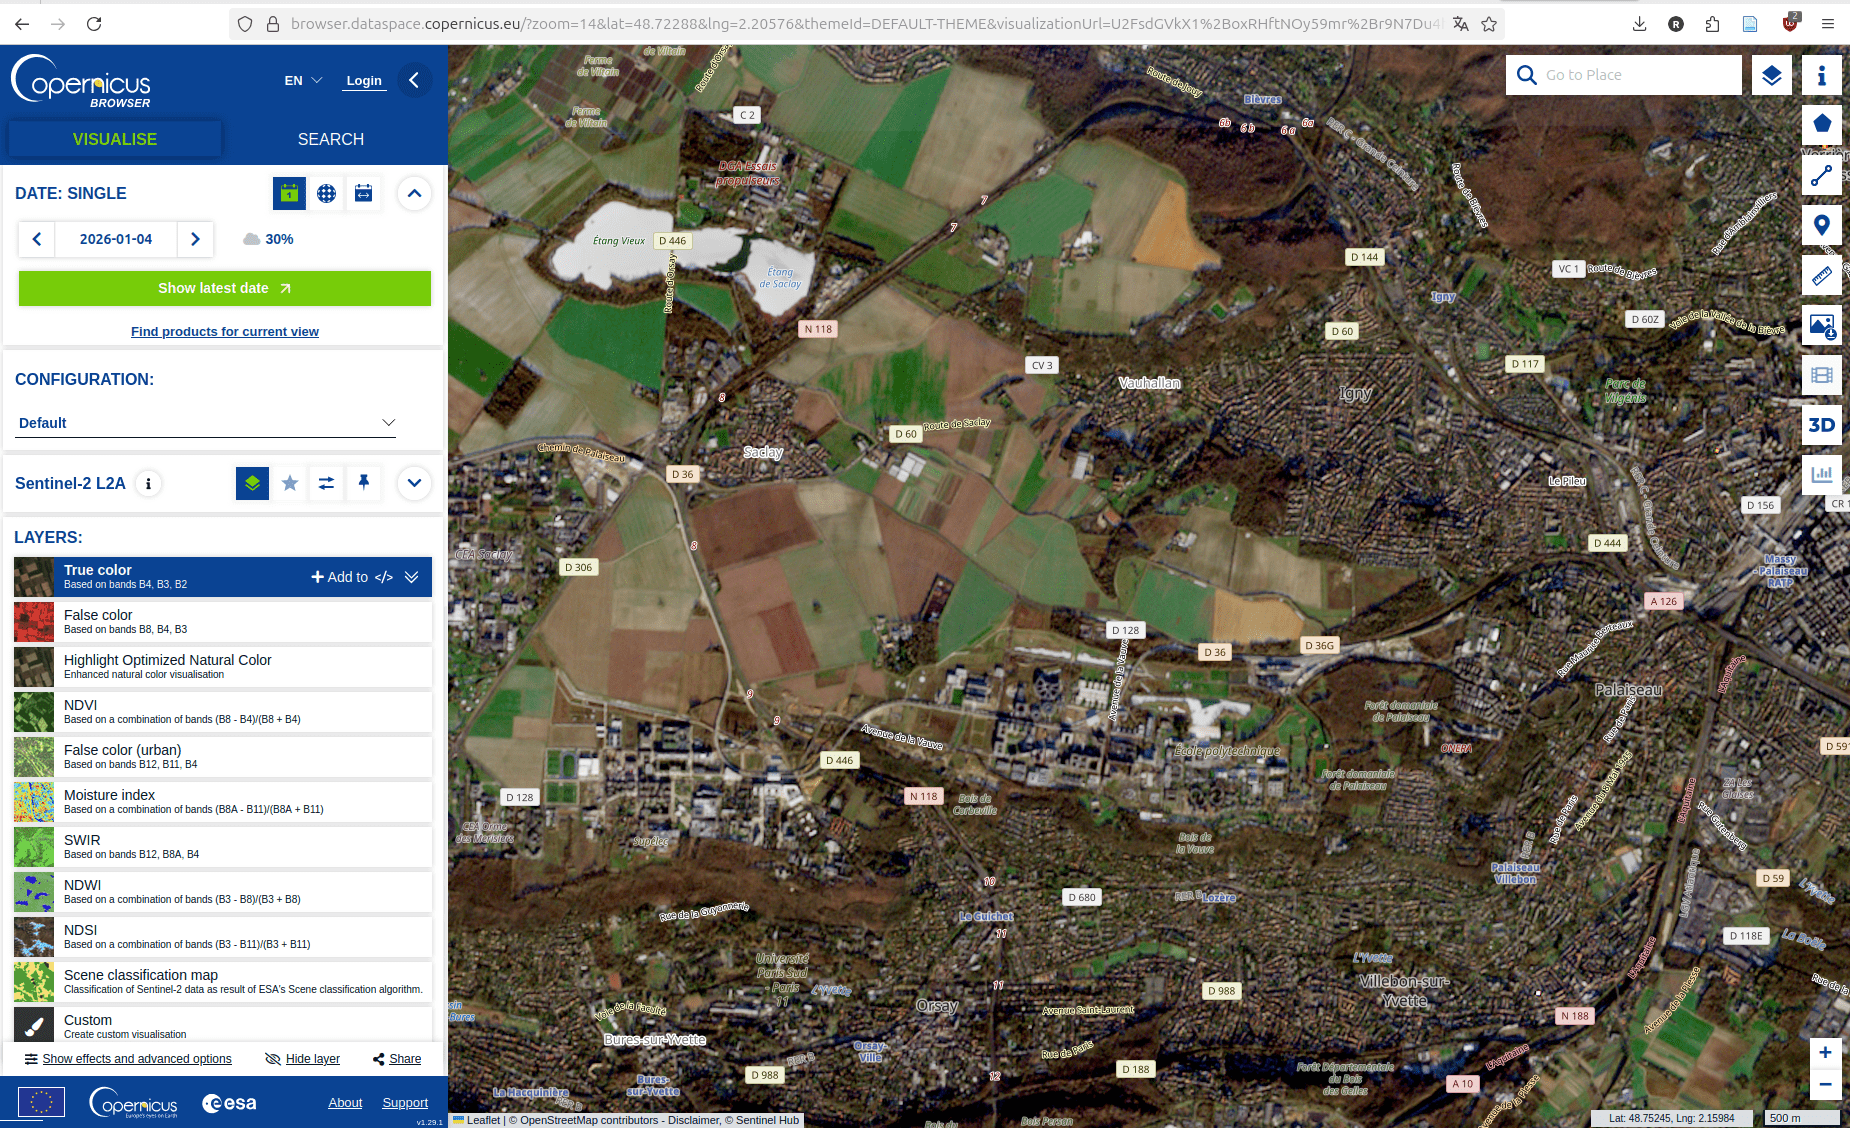
\includegraphics[width=0.95\textwidth]{figures/copernicus_browser.png}
		\caption{\url{https://browser.dataspace.copernicus.eu}}
	\end{subfigure}
\end{figure}

\end{frame}
%--------------------------------------------------------------------------
\begin{frame}{Sentinel-2 orbit}

Two satellites (currently three) are on a sun-synchronous orbit, allowing a global coverage at spatial resolution from 10m to 60m, and a revisit time of 5 days at the equator.

\begin{figure}
	\center
	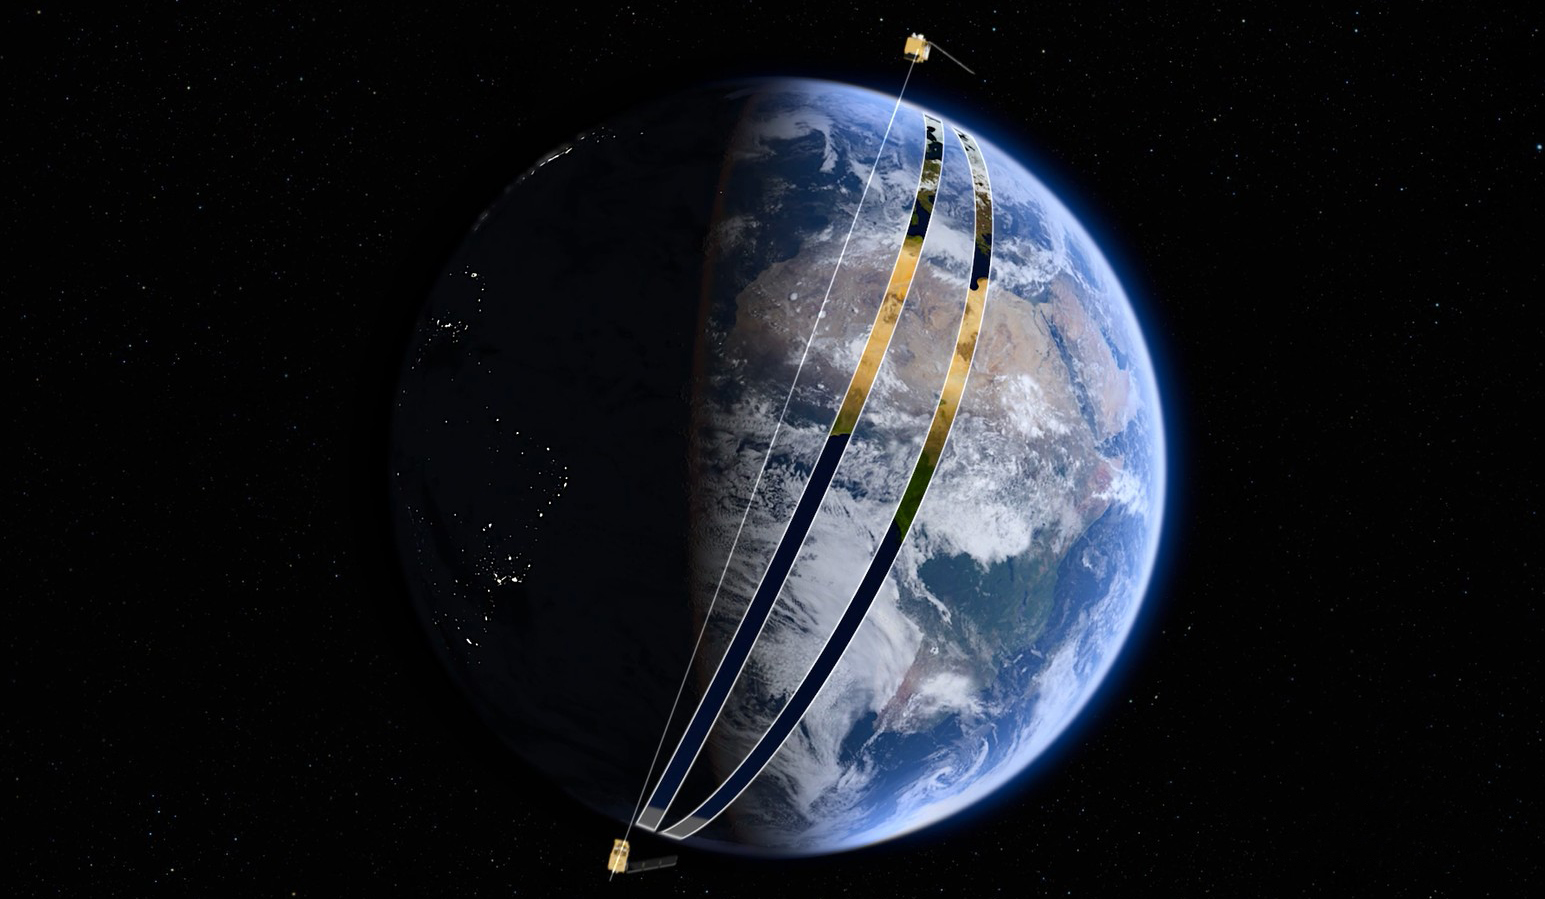
\includegraphics[width=0.6\textwidth]{figures/Sentinel-2_global_coverage.jpg
}
	\caption{"The Sentinel-2 mission is based on a constellation of two satellites orbiting 180° apart, which along with their 290 km-wide swaths, allows Earth’s main land surfaces, large islands, inland and coastal waters to be covered every five days." Credit:  ESA/ATG medialab}
\end{figure}



\end{frame}
%--------------------------------------------------------------------------
\begin{frame}{Spectral and temporal resolution of Sentinel-2}


\begin{figure}
	\center
	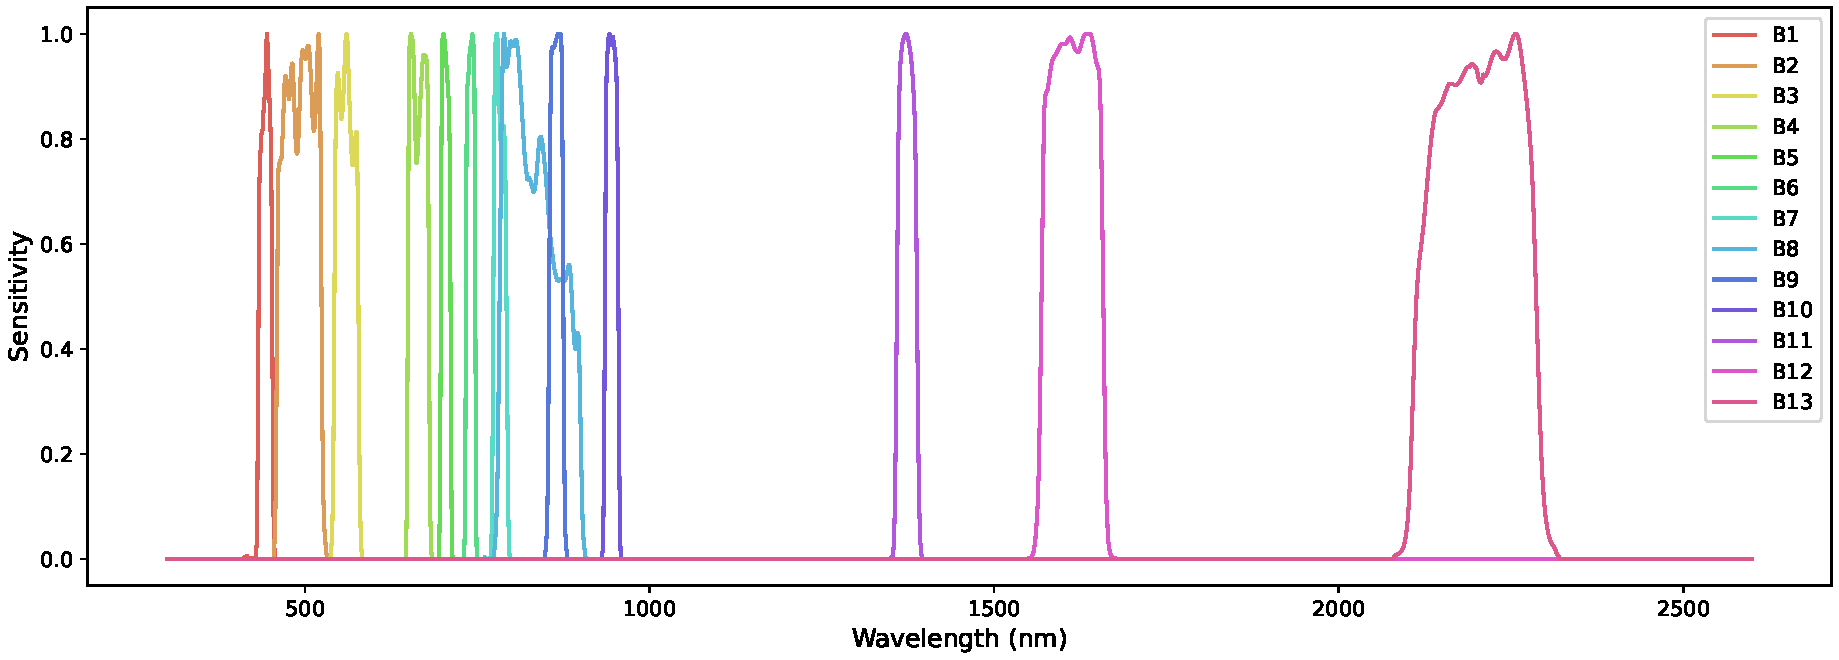
\includegraphics[width=0.6\textwidth]{figures/s2_sfr.pdf}
	\caption{Spectral sensitivity of the Sentinel-2 sensor. The multispectral instrument has 13 bands (or spectral channels) from the visible to the short-wave infrared (SWIR).}
\end{figure}

\begin{figure}
	\center
	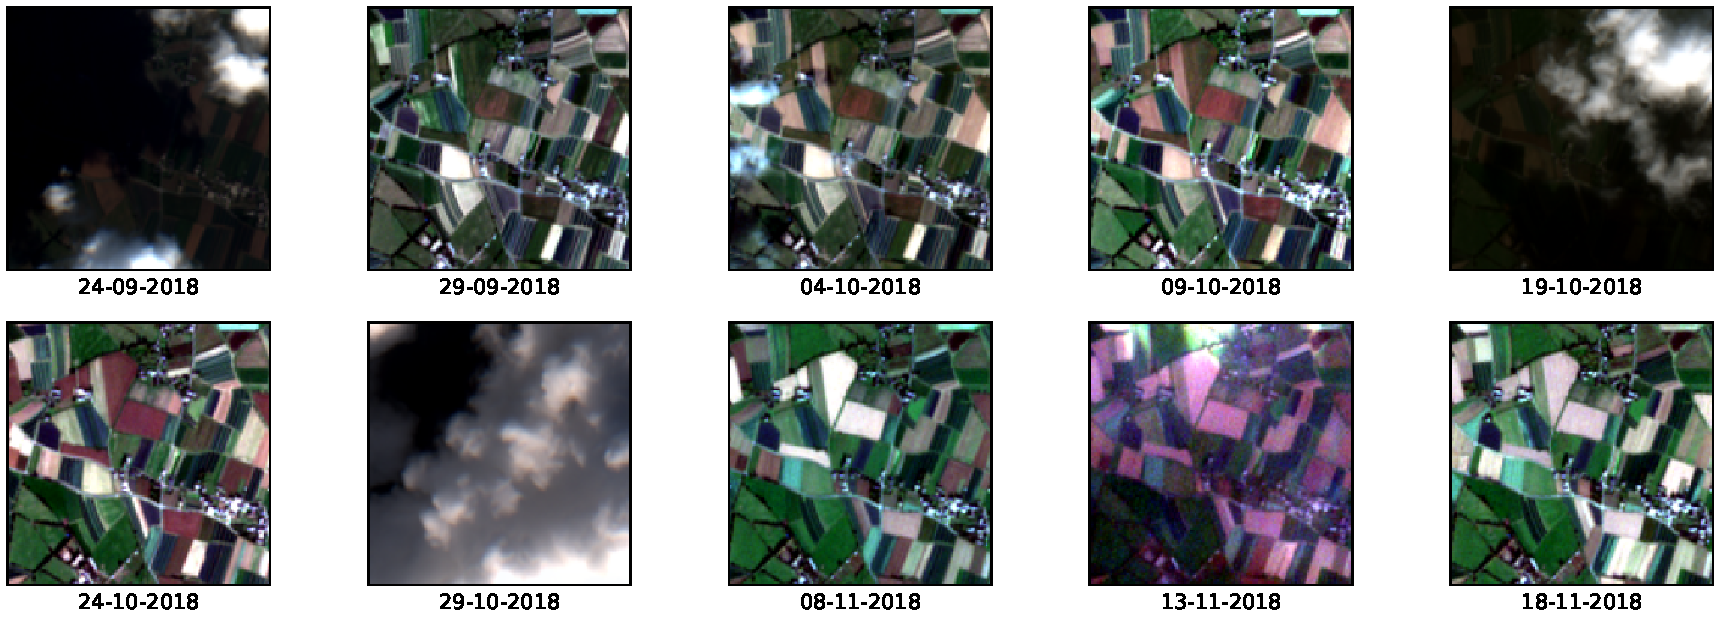
\includegraphics[width=0.6\textwidth]{figures/s2_ts.pdf}
	\caption{RGB composition of a Sentinel-2 (ESA, Copernicus) time series.}
\end{figure}

\end{frame}
%--------------------------------------------------------------
\begin{frame}
	Let's start coding!
\end{frame}
%--------------------------------------------------------------------------
%\begin{frame}[allowframebreaks,noframenumbering]
%\frametitle{}
%	\scriptsize{
%	\bibliographystyle{apalike}
%	\bibliography{main}}
%\end{frame}

\end{document}
